%%%%%%%%%%%%%%%%%%%%%%%%%%%%%%%%%%%%%%%%%%%%%%%%%%%%%%%%%%%%%%%%%%%%%%%%%%%%%%%
% MUSIC SYNC APP - ARCHITECTURE DOCUMENTATION
% LaTeX Version (Extended)
% Generated: December 19, 2025
%%%%%%%%%%%%%%%%%%%%%%%%%%%%%%%%%%%%%%%%%%%%%%%%%%%%%%%%%%%%%%%%%%%%%%%%%%%%%%%

\documentclass[11pt, a4paper]{report}

%------------------------------------------------------------------------------
% PACKAGES
%------------------------------------------------------------------------------
\usepackage[utf8]{inputenc}
\usepackage[T1]{fontenc}
\usepackage{lmodern}
\usepackage[margin=1in, headheight=14pt]{geometry}
\usepackage{textcomp}
\usepackage{graphicx}
\usepackage{xcolor}
\usepackage{hyperref}
\usepackage{listings}
\usepackage{booktabs}
\usepackage{longtable}
\usepackage{array}
\usepackage{tabularx}
\usepackage{multirow}
\usepackage{fancyhdr}
\usepackage{titlesec}
\usepackage{tocloft}
\usepackage{enumitem}
\usepackage{fancyvrb}
\usepackage{tcolorbox}
\usepackage{fontawesome5}
\usepackage{tikz}
\usepackage{pifont}
\usetikzlibrary{shapes.geometric, arrows, positioning, calc}

%------------------------------------------------------------------------------
% COLORS
%------------------------------------------------------------------------------
\definecolor{codebackground}{RGB}{245, 245, 245}
\definecolor{codeborder}{RGB}{200, 200, 200}
\definecolor{linkcolor}{RGB}{0, 102, 204}
\definecolor{sectioncolor}{RGB}{26, 26, 46}
\definecolor{accentcolor}{RGB}{102, 126, 234}
\definecolor{warningcolor}{RGB}{255, 193, 7}
\definecolor{successcolor}{RGB}{72, 187, 120}
\definecolor{infocolor}{RGB}{23, 162, 184}
\definecolor{errorcolor}{RGB}{220, 53, 69}

%------------------------------------------------------------------------------
% CUSTOM COMMANDS
%------------------------------------------------------------------------------
\newcommand{\inlinecode}[1]{\texttt{\colorbox{codebackground}{#1}}}
\newcommand{\filepath}[1]{\texttt{#1}}
\newcommand{\techterm}[1]{\textbf{#1}}
\newcommand{\cmark}{\ding{51}}
\newcommand{\xmark}{\ding{55}}

%------------------------------------------------------------------------------
% HYPERLINKS
%------------------------------------------------------------------------------
\hypersetup{
    colorlinks=true,
    linkcolor=linkcolor,
    filecolor=linkcolor,
    urlcolor=linkcolor,
    pdftitle={Music Sync App - Architecture Documentation},
    pdfauthor={Abdullahu5mani},
    pdfsubject={Electron Application Architecture},
    pdfkeywords={Electron, React, TypeScript, Music Player}
}

%------------------------------------------------------------------------------
% CODE LISTINGS
%------------------------------------------------------------------------------
\lstset{
    backgroundcolor=\color{codebackground},
    basicstyle=\ttfamily\small,
    breakatwhitespace=false,
    breaklines=true,
    captionpos=b,
    frame=single,
    framerule=0.5pt,
    rulecolor=\color{codeborder},
    keepspaces=true,
    numbers=none,
    showspaces=false,
    showstringspaces=false,
    showtabs=false,
    tabsize=2,
    xleftmargin=0.5em,
    xrightmargin=0.5em,
    aboveskip=1em,
    belowskip=1em
}

\lstdefinelanguage{TypeScript}{
    keywords={const, let, var, function, return, if, else, for, while, class, interface, type, export, import, from, async, await, new, this, extends, implements, public, private, protected, static, readonly, enum, true, false, null, undefined, void, any, string, number, boolean, object},
    keywordstyle=\color{blue}\bfseries,
    ndkeywords={useState, useEffect, useCallback, useMemo, useRef},
    ndkeywordstyle=\color{accentcolor}\bfseries,
    identifierstyle=\color{black},
    sensitive=true,
    comment=[l]{//},
    morecomment=[s]{/*}{*/},
    commentstyle=\color{gray}\itshape,
    stringstyle=\color{red},
    morestring=[b]',
    morestring=[b]"
}

%------------------------------------------------------------------------------
% TCOLORBOX ENVIRONMENTS
%------------------------------------------------------------------------------
\tcbuselibrary{skins, breakable}

\newtcolorbox{infobox}{
    colback=infocolor!10,
    colframe=infocolor,
    fonttitle=\bfseries,
    title={\faInfoCircle\ Note},
    breakable
}

\newtcolorbox{warningbox}{
    colback=warningcolor!10,
    colframe=warningcolor,
    fonttitle=\bfseries,
    title={\faExclamationTriangle\ Warning},
    breakable
}

\newtcolorbox{tipbox}{
    colback=successcolor!10,
    colframe=successcolor,
    fonttitle=\bfseries,
    title={\faLightbulb\ Tip},
    breakable
}

%------------------------------------------------------------------------------
% PAGE STYLE
%------------------------------------------------------------------------------
\pagestyle{fancy}
\fancyhf{}
\fancyhead[L]{\leftmark}
\fancyhead[R]{Music Sync App}
\fancyfoot[C]{\thepage}
\renewcommand{\headrulewidth}{0.4pt}
\renewcommand{\footrulewidth}{0.4pt}

%------------------------------------------------------------------------------
% SECTION FORMATTING
%------------------------------------------------------------------------------
\titleformat{\chapter}[display]
    {\normalfont\huge\bfseries\color{sectioncolor}}
    {\chaptertitlename\ \thechapter}{20pt}{\Huge}
\titleformat{\section}
    {\normalfont\Large\bfseries\color{sectioncolor}}
    {\thesection}{1em}{}
\titleformat{\subsection}
    {\normalfont\large\bfseries\color{sectioncolor}}
    {\thesubsection}{1em}{}

%------------------------------------------------------------------------------
% DOCUMENT BEGIN
%------------------------------------------------------------------------------
\begin{document}

%------------------------------------------------------------------------------
% TITLE PAGE
%------------------------------------------------------------------------------
\begin{titlepage}
    \centering
    \vspace*{2cm}
    
    {\Huge\bfseries\color{sectioncolor} Music Sync App\par}
    \vspace{0.5cm}
    {\LARGE Architecture Documentation\par}
    \vspace{2cm}
    
    \begin{tikzpicture}
        \node[draw=accentcolor, line width=2pt, rounded corners=10pt, 
              inner sep=20pt, fill=accentcolor!10] {
            \begin{minipage}{0.6\textwidth}
                \centering
                {\Large\faMusic\ \faReact\ \faNodeJs\par}
                \vspace{0.5cm}
                {\normalsize Electron + React + TypeScript\par}
                {\normalsize Desktop Music Player\par}
            \end{minipage}
        };
    \end{tikzpicture}
    
    \vspace{2cm}
    
    {\large\itshape A comprehensive guide for developers\par}
    \vspace{0.5cm}
    {\normalsize Written for developers new to Electron\par}
    
    \vfill
    
    {\normalsize Version 0.0.1\par}
    {\normalsize December 2025\par}
    \vspace{1cm}
    {\small Author: Abdullahu5mani\par}
    {\small Repository: \url{https://github.com/Abdullahu5mani/Music-Electron-App}\par}
\end{titlepage}

%------------------------------------------------------------------------------
% TABLE OF CONTENTS
%------------------------------------------------------------------------------
\tableofcontents
\newpage

%%%%%%%%%%%%%%%%%%%%%%%%%%%%%%%%%%%%%%%%%%%%%%%%%%%%%%%%%%%%%%%%%%%%%%%%%%%%%%%
% CHAPTER 1: QUICK START GUIDE
%%%%%%%%%%%%%%%%%%%%%%%%%%%%%%%%%%%%%%%%%%%%%%%%%%%%%%%%%%%%%%%%%%%%%%%%%%%%%%%
\chapter{Quick Start Guide (For Beginners)}
\label{ch:quickstart}

\begin{infobox}
This guide is written for developers new to Electron. If you're experienced with Electron, you can skip to Chapter~\ref{ch:architecture}.
\end{infobox}

\section{The Two Worlds of Electron}

Think of this app as having two separate programs running at the same time:

\begin{table}[h!]
\centering
\begin{tabular}{@{}p{2cm}p{2.5cm}p{7cm}p{2.5cm}@{}}
\toprule
\textbf{World} & \textbf{Folder} & \textbf{What it does} & \textbf{Technology} \\
\midrule
\textbf{Backend} & \filepath{electron/} & Handles system stuff (files, downloads, database) & Node.js \\
\textbf{Frontend} & \filepath{src/} & Shows the UI (buttons, lists, player) & React \\
\bottomrule
\end{tabular}
\caption{The Two Worlds of an Electron Application}
\end{table}

These two worlds \textbf{cannot directly talk to each other} for security. They communicate through a ``bridge'' called the \techterm{Preload Script}.

\section{File Map: What Does What?}

\subsection{Electron Backend (Node.js)}

\begin{longtable}{@{}p{4.5cm}p{10cm}@{}}
\toprule
\textbf{File} & \textbf{Purpose} \\
\midrule
\endhead

\filepath{electron/main.ts} & \textbf{ENTRY POINT} --- Creates the app window, starts everything \\
\filepath{electron/preload.ts} & \textbf{THE BRIDGE} --- Safely exposes backend functions to frontend \\
\filepath{electron/window.ts} & Creates app window with custom title bar \\
\filepath{electron/tray.ts} & System tray icon with play/pause controls \\
\filepath{electron/musicScanner.ts} & Finds music files and reads metadata \\
\filepath{electron/parallelMetadataScanner.ts} & Multi-threaded metadata parsing \\
\filepath{electron/fileWatcher.ts} & Monitors music folder in real-time \\
\filepath{electron/metadataCache.ts} & SQLite cache for scan tracking \\
\filepath{electron/youtubeDownloader.ts} & Downloads audio from YouTube \\
\filepath{electron/playlistDatabase.ts} & SQLite database for playlists \\
\filepath{electron/whisperManager.ts} & AI transcription system \\
\filepath{electron/fpcalcManager.ts} & Audio fingerprinting \\
\filepath{electron/binaryManager.ts} & Binary status checking \\
\bottomrule
\caption{Electron Backend Files}
\end{longtable}

\subsection{IPC Handler Modules}

Located in \filepath{electron/ipc/modules/}:

\begin{table}[h!]
\centering
\begin{tabular}{@{}p{4cm}p{8cm}@{}}
\toprule
\textbf{Module} & \textbf{Handles} \\
\midrule
\filepath{musicHandlers.ts} & Scanning folders, reading files \\
\filepath{playlistHandlers.ts} & Create/delete/update playlists \\
\filepath{youtubeHandlers.ts} & Download from YouTube, binary installs \\
\filepath{apiHandlers.ts} & External APIs (AcoustID, MusicBrainz) \\
\filepath{systemHandlers.ts} & Window controls (minimize, close) \\
\filepath{cacheHandlers.ts} & Metadata database operations \\
\filepath{fingerprintHandlers.ts} & Audio fingerprinting (fpcalc) \\
\filepath{lyricsHandlers.ts} & Vocal isolation + AI transcription \\
\filepath{watchHandlers.ts} & File system watching \\
\bottomrule
\end{tabular}
\caption{IPC Handler Modules}
\end{table}

\section{How Data Flows: Playing a Song}

\begin{enumerate}
    \item \textbf{User clicks a song in SongList.tsx}
    \begin{itemize}
        \item Calls \inlinecode{onPlaySong(file, index)}
    \end{itemize}
    
    \item \textbf{App.tsx receives the call}
    \begin{itemize}
        \item Calls \inlinecode{playSong(file, index)} from \inlinecode{useAudioPlayer} hook
    \end{itemize}
    
    \item \textbf{useAudioPlayer.ts processes the request}
    \begin{itemize}
        \item Creates new \inlinecode{Howl(\{ src: 'file://path/to/song.mp3' \})}
        \item Calls \inlinecode{sound.play()}
        \item Updates state: \inlinecode{setIsPlaying(true)}
    \end{itemize}
    
    \item \textbf{React re-renders}
    \begin{itemize}
        \item PlaybackBar shows the song title, artist, album art
        \item SongList highlights the playing song
        \item AudioVisualizer starts animating
    \end{itemize}
\end{enumerate}

%%%%%%%%%%%%%%%%%%%%%%%%%%%%%%%%%%%%%%%%%%%%%%%%%%%%%%%%%%%%%%%%%%%%%%%%%%%%%%%
% CHAPTER 2: OVERVIEW
%%%%%%%%%%%%%%%%%%%%%%%%%%%%%%%%%%%%%%%%%%%%%%%%%%%%%%%%%%%%%%%%%%%%%%%%%%%%%%%
\chapter{Overview}
\label{ch:overview}

This is an \textbf{Electron + React + TypeScript} desktop music player application. It allows users to:

\begin{itemize}
    \item Browse and play local music files
    \item Download music from YouTube using \inlinecode{yt-dlp}
    \item Control playback from the system tray
    \item Identify songs using audio fingerprinting (AcoustID + MusicBrainz)
    \item Custom frameless window with a soft blue title bar
    \item Filter library by artist/album via sidebar
    \item Create and manage playlists
    \item Generate AI-powered lyrics using Whisper transcription
\end{itemize}

\section{Tech Stack}

\begin{longtable}{@{}p{3.5cm}p{4.5cm}p{6cm}@{}}
\toprule
\textbf{Layer} & \textbf{Technology} & \textbf{Purpose} \\
\midrule
\endhead

Runtime & Electron 39 & Desktop app framework \\
Frontend & React 18 + TypeScript & UI components \\
Build Tool & Vite 7 & Fast dev server and bundling \\
Audio Playback & Howler.js & Cross-platform audio \\
Metadata & music-metadata & Extract ID3 tags and album art \\
YouTube & yt-dlp-wrap & Download audio from YouTube \\
Audio Fingerprinting & fpcalc (Chromaprint) & Generate audio fingerprints \\
Audio Processing & FFmpeg & Vocal isolation, format conversion \\
AI Transcription & Whisper.cpp & Speech-to-text for lyrics \\
Tag Writing & taglib-wasm & Write cover art to files \\
Database & better-sqlite3 & SQLite metadata cache \\
Sliders & rc-slider & Seek bar and volume control \\
Scrollbars & overlayscrollbars-react & Custom themed scrollbars \\
HTTP & axios & API requests \\
Styling & CSS (no framework) & Custom responsive design \\
\bottomrule
\caption{Technology Stack}
\end{longtable}

\section{Supported Audio Formats}

\filepath{.mp3}, \filepath{.flac}, \filepath{.wav}, \filepath{.m4a}, \filepath{.aac}, \filepath{.ogg}, \filepath{.opus}, \filepath{.wma}, \filepath{.aiff}, \filepath{.mp4}, \filepath{.m4p}, \filepath{.amr}

\section{Directory Structure}

\begin{lstlisting}
music-electron-app/
+-- electron/                 # Main Process (Node.js)
|   +-- main.ts              # App entry point
|   +-- preload.ts           # IPC bridge
|   +-- window.ts            # Window creation
|   +-- tray.ts              # System tray
|   +-- musicScanner.ts      # File discovery
|   +-- metadataCache.ts     # SQLite scan cache
|   +-- playlistDatabase.ts  # SQLite playlists
|   +-- youtubeDownloader.ts # yt-dlp wrapper
|   +-- fpcalcManager.ts     # Audio fingerprinting
|   +-- whisperManager.ts    # AI transcription
|   +-- settings.ts          # Settings persistence
|   +-- ipc/
|       +-- handlers.ts      # Handler registry
|       +-- modules/         # Feature-specific handlers
+-- src/                     # Renderer Process (React)
|   +-- main.tsx            # React entry
|   +-- App.tsx             # Main component
|   +-- hooks/              # Custom React hooks
|   +-- components/         # UI components
|   |   +-- layout/         # TitleBar, Sidebar, PlaybackBar
|   |   +-- library/        # SongList, BatchScanProgress
|   |   +-- playlists/      # PlaylistList, CreatePlaylistModal
|   |   +-- lyrics/         # LyricsPanel
|   |   +-- common/         # AudioVisualizer, ContextMenu
|   |   +-- settings/       # Settings modal
|   |   +-- download/       # DownloadButton, Notification
|   +-- services/           # API wrappers
|   +-- utils/              # Helper functions
|   +-- assets/icons/       # 39 custom SVG icons
+-- package.json
+-- vite.config.ts
+-- electron-builder.json5
\end{lstlisting}

%%%%%%%%%%%%%%%%%%%%%%%%%%%%%%%%%%%%%%%%%%%%%%%%%%%%%%%%%%%%%%%%%%%%%%%%%%%%%%%
% CHAPTER 3: ARCHITECTURE
%%%%%%%%%%%%%%%%%%%%%%%%%%%%%%%%%%%%%%%%%%%%%%%%%%%%%%%%%%%%%%%%%%%%%%%%%%%%%%%
\chapter{High-Level Architecture}
\label{ch:architecture}

\section{Two-Process Architecture}

\begin{figure}[h!]
\centering
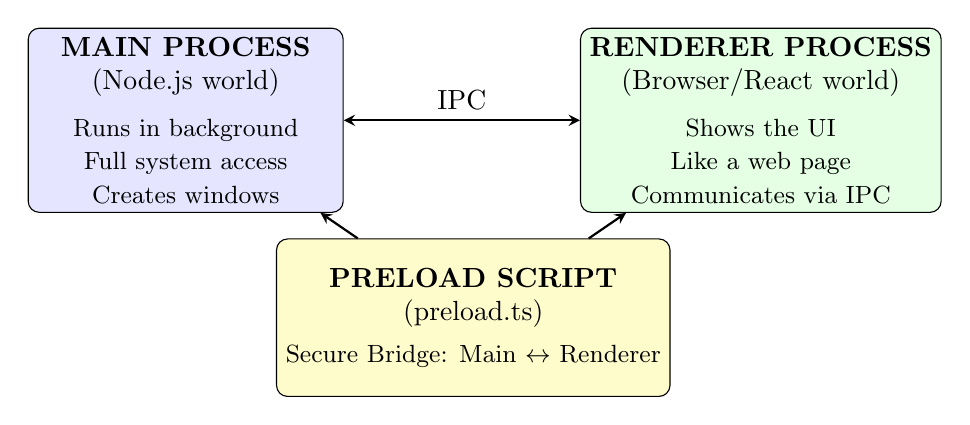
\begin{tikzpicture}[
    node distance=2cm,
    box/.style={draw, rounded corners, minimum width=4cm, minimum height=2cm, align=center, fill=white},
    arrow/.style={->, thick, >=stealth}
]
    % Main Process
    \node[box, fill=blue!10] (main) {
        \textbf{MAIN PROCESS}\\
        (Node.js world)\\[0.5em]
        \small Runs in background\\
        \small Full system access\\
        \small Creates windows
    };
    
    % Renderer Process
    \node[box, fill=green!10, right=3cm of main] (renderer) {
        \textbf{RENDERER PROCESS}\\
        (Browser/React world)\\[0.5em]
        \small Shows the UI\\
        \small Like a web page\\
        \small Communicates via IPC
    };
    
    % IPC Arrow
    \draw[arrow, <->] (main) -- node[above] {IPC} (renderer);
    
    % Preload Script
    \node[box, fill=yellow!20, below=1.5cm of $(main)!0.5!(renderer)$] (preload) {
        \textbf{PRELOAD SCRIPT}\\
        (preload.ts)\\[0.3em]
        \small Secure Bridge: Main $\leftrightarrow$ Renderer
    };
    
    \draw[arrow] (preload) -- (main);
    \draw[arrow] (preload) -- (renderer);
    
\end{tikzpicture}
\caption{Electron Two-Process Architecture}
\end{figure}

%%%%%%%%%%%%%%%%%%%%%%%%%%%%%%%%%%%%%%%%%%%%%%%%%%%%%%%%%%%%%%%%%%%%%%%%%%%%%%%
% CHAPTER 4: IPC COMMUNICATION
%%%%%%%%%%%%%%%%%%%%%%%%%%%%%%%%%%%%%%%%%%%%%%%%%%%%%%%%%%%%%%%%%%%%%%%%%%%%%%%
\chapter{IPC Communication}
\label{ch:ipc}

Handlers are organized into \textbf{modular files} for better maintainability.

\section{All IPC Endpoints}

\begin{longtable}{@{}p{3cm}p{4.5cm}p{1.5cm}p{5.5cm}@{}}
\toprule
\textbf{Module} & \textbf{Handler} & \textbf{Type} & \textbf{Purpose} \\
\midrule
\endhead

musicHandlers & \inlinecode{scan-music-folder} & invoke & Scan directory for music files \\
& \inlinecode{select-music-folder} & invoke & Open folder selection dialog \\
& \inlinecode{read-single-file-metadata} & invoke & Read metadata for a single file \\
& \inlinecode{write-cover-art} & invoke & Embed cover art in audio file \\
& \inlinecode{write-metadata} & invoke & Write all metadata to audio file \\
\addlinespace

apiHandlers & \inlinecode{lookup-acoustid} & invoke & Query AcoustID API \\
& \inlinecode{lookup-musicbrainz} & invoke & Query MusicBrainz API \\
& \inlinecode{download-image} & invoke & Download cover art image \\
& \inlinecode{download-image-with-fallback} & invoke & Download cover art with fallback URLs \\
\addlinespace

youtubeHandlers & \inlinecode{download-youtube} & invoke & Download audio from YouTube \\
& \inlinecode{get-binary-statuses} & invoke & Get status of yt-dlp binary \\
\addlinespace

systemHandlers & \inlinecode{window-minimize} & on & Minimize window \\
& \inlinecode{window-maximize} & on & Toggle maximize/restore \\
& \inlinecode{window-close} & on & Close window \\
& \inlinecode{get-settings} & invoke & Get stored settings from disk \\
& \inlinecode{save-settings} & invoke & Save settings to disk \\
\addlinespace

cacheHandlers & \inlinecode{cache-get-file-status} & invoke & Get scan status for a file \\
& \inlinecode{cache-mark-file-scanned} & invoke & Record scan result in database \\
& \inlinecode{cache-get-batch-status} & invoke & Get status for multiple files \\
& \inlinecode{cache-get-statistics} & invoke & Get total/tagged/untagged counts \\
\addlinespace

fingerprintHandlers & \inlinecode{generate-fingerprint} & invoke & Generate AcoustID fingerprint \\
& \inlinecode{fingerprint-check-ready} & invoke & Check if fpcalc is installed \\
\addlinespace

playlistHandlers & \inlinecode{playlist-create} & invoke & Create a new playlist \\
& \inlinecode{playlist-delete} & invoke & Delete a playlist \\
& \inlinecode{playlist-get-all} & invoke & Get all playlists \\
& \inlinecode{playlist-add-songs} & invoke & Add songs to a playlist \\
& \inlinecode{playlist-remove-song} & invoke & Remove a song from a playlist \\
\bottomrule
\caption{All IPC Endpoints}
\end{longtable}

%%%%%%%%%%%%%%%%%%%%%%%%%%%%%%%%%%%%%%%%%%%%%%%%%%%%%%%%%%%%%%%%%%%%%%%%%%%%%%%
% CHAPTER 5: EXTERNAL API INTEGRATION
%%%%%%%%%%%%%%%%%%%%%%%%%%%%%%%%%%%%%%%%%%%%%%%%%%%%%%%%%%%%%%%%%%%%%%%%%%%%%%%
\chapter{External API Integration}
\label{ch:api}

\section{Rate Limiting}

API calls are rate-limited to respect external service limits.

\begin{table}[h!]
\centering
\begin{tabular}{@{}p{3cm}p{4cm}p{3.5cm}p{3.5cm}@{}}
\toprule
\textbf{API} & \textbf{Limit} & \textbf{Our Delay} & \textbf{Safety Margin} \\
\midrule
\textbf{AcoustID} & 3 req/sec & 500ms & $\sim$2 req/sec \\
\textbf{MusicBrainz} & 1 req/sec & 1100ms & Buffer for latency \\
\textbf{Cover Art Archive} & 1 req/sec & 1100ms & Same as MusicBrainz \\
\textbf{Between Songs} & N/A & 500ms & Prevent API hammering \\
\bottomrule
\end{tabular}
\caption{API Rate Limiting}
\end{table}

\section{Cover Art Fallback System}

The Cover Art Archive often returns 404 for specific releases. The app tries multiple URLs in priority order:

\begin{enumerate}
    \item \textbf{250px front cover} for each release (best quality/size ratio)
    \item \textbf{500px front cover} for each release (higher quality)
    \item \textbf{Original size} for each release (largest)
    \item \textbf{Release group} fallback (if all releases fail)
\end{enumerate}

\section{Fingerprint + Tag Flow}

Fingerprinting runs in the \textbf{Main Process} using the \inlinecode{fpcalc} binary:

\begin{enumerate}
    \item User clicks ``Identify Song'' button
    \item Check cache --- if already scanned, skip
    \item Generate fingerprint via \inlinecode{fpcalc} (subprocess)
    \item Lookup fingerprint on AcoustID API
    \item If match found, query MusicBrainz for metadata
    \item Download cover art with fallback URLs
    \item Write metadata to audio file (taglib-wasm)
    \item Mark file as scanned in cache
    \item Update UI in-place (no full library refresh)
\end{enumerate}

%%%%%%%%%%%%%%%%%%%%%%%%%%%%%%%%%%%%%%%%%%%%%%%%%%%%%%%%%%%%%%%%%%%%%%%%%%%%%%%
% CHAPTER 6: SECURITY ARCHITECTURE
%%%%%%%%%%%%%%%%%%%%%%%%%%%%%%%%%%%%%%%%%%%%%%%%%%%%%%%%%%%%%%%%%%%%%%%%%%%%%%%
\chapter{Security Architecture}
\label{ch:security}

\section{Process Isolation (contextBridge)}

We strictly enforce \textbf{Context Isolation} to prevent the Renderer from directly accessing Node.js primitives.

\begin{itemize}
    \item \textbf{Renderer Context:}
    \begin{itemize}
        \item Has \textbf{no} access to \inlinecode{require()}, \inlinecode{process}, or \inlinecode{fs}
        \item Can only communicate via \inlinecode{window.electronAPI}
    \end{itemize}
    
    \item \textbf{Preload Script:}
    \begin{itemize}
        \item Acts as a privileged intermediary
        \item Exposes only safe, typed functions
        \item Sanitizes IPC inputs before passing to Main
    \end{itemize}
\end{itemize}

\section{Local File Access \& webSecurity}

\textbf{Current Trade-off:} The application sets \inlinecode{webSecurity: false} in \filepath{window.ts}.

\begin{lstlisting}[language=TypeScript]
webPreferences: {
  webSecurity: false,           // Allows file:// access
  allowRunningInsecureContent: true
}
\end{lstlisting}

\textbf{Rationale:}
\begin{itemize}
    \item \textbf{Requirement:} Howler.js and \inlinecode{<img>} tags need to load local audio/image files
    \item \textbf{Mitigation:} Remote content is strictly limited; external images downloaded to local storage first
    \item \textbf{NodeIntegration} remains \textbf{disabled}
\end{itemize}

\section{IPC Security}

\begin{itemize}
    \item \textbf{Channel Whitelisting:} Only specific, hardcoded channels are exposed
    \item \textbf{Payload Validation:} Handlers validate paths for basic sanity checks
\end{itemize}

%%%%%%%%%%%%%%%%%%%%%%%%%%%%%%%%%%%%%%%%%%%%%%%%%%%%%%%%%%%%%%%%%%%%%%%%%%%%%%%
% CHAPTER 7: MULTITHREADED ARCHITECTURE
%%%%%%%%%%%%%%%%%%%%%%%%%%%%%%%%%%%%%%%%%%%%%%%%%%%%%%%%%%%%%%%%%%%%%%%%%%%%%%%
\chapter{Multithreaded Architecture}
\label{ch:multithreaded}

The application uses two distinct worker pool systems to maximize CPU utilization.

\section{Worker Pool Systems}

\begin{table}[h!]
\centering
\begin{tabular}{@{}p{4cm}p{5cm}p{5cm}@{}}
\toprule
\textbf{System} & \textbf{Purpose} & \textbf{Workers} \\
\midrule
ParallelMetadataScanner & Metadata parsing & 15 concurrent parsers \\
FingerprintWorkerPool & Audio fingerprinting & 15 concurrent fpcalc \\
\bottomrule
\end{tabular}
\caption{Worker Pool Systems}
\end{table}

\section{Data Flow}

\begin{enumerate}
    \item \textbf{Startup} --- App loads, scans music folder
    \item \textbf{Parallel Metadata Scan} --- 15 workers parse metadata simultaneously
    \item \textbf{User initiates batch scan} --- Fingerprint worker pool spins up
    \item \textbf{API lookups} --- Rate-limited queries to AcoustID and MusicBrainz
    \item \textbf{Metadata writing} --- taglib-wasm embeds cover art and metadata
\end{enumerate}

\section{Key Storage Locations}

\begin{table}[h!]
\centering
\begin{tabular}{@{}p{4cm}p{5cm}p{5cm}@{}}
\toprule
\textbf{Data} & \textbf{Storage} & \textbf{Persistence} \\
\midrule
Fingerprints & Memory (RAM) only & Temporary \\
fpcalc binary & \filepath{\%APPDATA\%/music-sync-app/binaries/} & Permanent \\
Scan status cache & \filepath{metadata-cache.db} (SQLite) & Permanent \\
Cover art images & \filepath{assets/*.jpg} & Temporary (deleted after embed) \\
Metadata & Embedded in audio files (ID3/Vorbis) & Permanent \\
\bottomrule
\end{tabular}
\caption{Data Storage Locations}
\end{table}

%%%%%%%%%%%%%%%%%%%%%%%%%%%%%%%%%%%%%%%%%%%%%%%%%%%%%%%%%%%%%%%%%%%%%%%%%%%%%%%
% CHAPTER 8: KEY DESIGN PATTERNS
%%%%%%%%%%%%%%%%%%%%%%%%%%%%%%%%%%%%%%%%%%%%%%%%%%%%%%%%%%%%%%%%%%%%%%%%%%%%%%%
\chapter{Key Design Patterns}
\label{ch:patterns}

\begin{enumerate}
    \item \textbf{Custom Hooks} --- Encapsulate complex logic (\inlinecode{useAudioPlayer}, \inlinecode{useMusicLibrary}, \inlinecode{useSongScanner})
    \item \textbf{Memoization} --- \inlinecode{useMemo} for sorted music files
    \item \textbf{Modular IPC Handlers} --- Split by feature for maintainability
    \item \textbf{Cleanup Functions} --- All IPC listeners return cleanup functions
    \item \textbf{Rate Limiting} --- Delays between API calls to respect service limits
    \item \textbf{Path Normalization} --- Cross-platform \inlinecode{file://} URL generation
    \item \textbf{SQLite Caching} --- Persistent scan tracking with file change detection
    \item \textbf{Hash-Based Change Detection} --- SHA256(path+size+mtime) for detecting file modifications
    \item \textbf{Fallback URL Strategy} --- Try multiple cover art URLs sequentially
    \item \textbf{Non-Blocking Notifications} --- Toast notifications without interrupting workflow
    \item \textbf{Release Scoring} --- Prioritize original albums over compilations
    \item \textbf{Batch Processing} --- Process multiple files with progress tracking and cancellation
    \item \textbf{Graceful Error Recovery} --- Auto-delete corrupted binaries, handle API failures
    \item \textbf{Circuit Breaker} --- Stop fingerprinting after consecutive failures
    \item \textbf{Subprocess Fingerprinting} --- Run fpcalc as separate process to avoid memory limits
    \item \textbf{On-Demand Binary Download} --- Download platform-specific binaries on first use
    \item \textbf{In-Place Metadata Updates} --- Update single file without full library refresh
    \item \textbf{Immediate Asset Cleanup} --- Delete temp cover art after embedding
\end{enumerate}

%%%%%%%%%%%%%%%%%%%%%%%%%%%%%%%%%%%%%%%%%%%%%%%%%%%%%%%%%%%%%%%%%%%%%%%%%%%%%%%
% CHAPTER 9: PLATFORM SUPPORT
%%%%%%%%%%%%%%%%%%%%%%%%%%%%%%%%%%%%%%%%%%%%%%%%%%%%%%%%%%%%%%%%%%%%%%%%%%%%%%%
\chapter{Cross-Platform Strategy}
\label{ch:platform}

\section{Platform Support Matrix}

\subsection{yt-dlp Binary --- Full Cross-Platform Support}

\begin{table}[h!]
\centering
\begin{tabular}{@{}p{3cm}p{4cm}p{3.5cm}p{3.5cm}@{}}
\toprule
\textbf{Platform} & \textbf{Architecture} & \textbf{Binary Name} & \textbf{Status} \\
\midrule
Windows & x64 & \filepath{yt-dlp.exe} & \cmark\ Supported \\
Windows & ARM64 & \filepath{yt-dlp\_win\_arm64.exe} & \cmark\ Supported \\
macOS & x64 (Intel) & \filepath{yt-dlp\_macos} & \cmark\ Supported \\
macOS & ARM64 (M1/M2/M3) & \filepath{yt-dlp\_macos\_arm64} & \cmark\ Supported \\
Linux & x64 & \filepath{yt-dlp\_linux} & \cmark\ Supported \\
Linux & ARM64 & \filepath{yt-dlp\_linux\_arm64} & \cmark\ Supported \\
\bottomrule
\end{tabular}
\caption{yt-dlp Platform Support}
\end{table}

\subsection{fpcalc Binary --- Partial ARM64 Support}

\begin{table}[h!]
\centering
\begin{tabular}{@{}p{3cm}p{4cm}p{3.5cm}p{3.5cm}@{}}
\toprule
\textbf{Platform} & \textbf{Architecture} & \textbf{Binary Name} & \textbf{Status} \\
\midrule
Windows & x64 & chromaprint-fpcalc-windows-x86\_64 & \cmark\ Supported \\
Windows & ARM64 & --- & \xmark\ Not available \\
macOS & x64 (Intel) & chromaprint-fpcalc-macos-x86\_64 & \cmark\ Supported \\
macOS & ARM64 (M1/M2/M3) & chromaprint-fpcalc-macos-arm64 & \cmark\ Supported \\
Linux & x64 & chromaprint-fpcalc-linux-x86\_64 & \cmark\ Supported \\
Linux & ARM64 & --- & \xmark\ Not available \\
\bottomrule
\end{tabular}
\caption{fpcalc Platform Support}
\end{table}

\begin{warningbox}
Chromaprint (fpcalc) project doesn't publish ARM64 builds for Windows or Linux. Audio fingerprinting features are unavailable on these platforms.
\end{warningbox}

\section{Feature Availability by Platform}

\begin{table}[h!]
\centering
\begin{tabular}{@{}p{3cm}p{4cm}p{3.5cm}p{3.5cm}@{}}
\toprule
\textbf{Platform} & \textbf{YouTube Download} & \textbf{Audio Fingerprinting} & \textbf{Metadata Tagging} \\
\midrule
Windows x64 & \cmark & \cmark & \cmark \\
Windows ARM64 & \cmark & \xmark\ No fpcalc & \cmark \\
macOS x64 & \cmark & \cmark & \cmark \\
macOS ARM64 & \cmark & \cmark & \cmark \\
Linux x64 & \cmark & \cmark & \cmark \\
Linux ARM64 & \cmark & \xmark\ No fpcalc & \cmark \\
\bottomrule
\end{tabular}
\caption{Feature Availability by Platform}
\end{table}

%%%%%%%%%%%%%%%%%%%%%%%%%%%%%%%%%%%%%%%%%%%%%%%%%%%%%%%%%%%%%%%%%%%%%%%%%%%%%%%
% CHAPTER 10: VISUAL ENHANCEMENTS
%%%%%%%%%%%%%%%%%%%%%%%%%%%%%%%%%%%%%%%%%%%%%%%%%%%%%%%%%%%%%%%%%%%%%%%%%%%%%%%
\chapter{Visual Enhancements}
\label{ch:visual}

\section{Dynamic Album Art Glow}

The playback bar features an animated glow effect that dynamically adapts to the currently playing album's colors.

\textbf{Implementation:}
\begin{itemize}
    \item \textbf{Color Extraction} (\filepath{colorExtractor.ts}): Samples album art using canvas pixel analysis
    \item \textbf{Conic Gradient Border}: Uses CSS \inlinecode{conic-gradient} with extracted colors
    \item \textbf{Ambient Animation}: 16-second animation with rotation, scale, blur, and opacity
    \item \textbf{Interactivity}: Animation pauses on hover; only active when music is playing
\end{itemize}

\begin{lstlisting}[language={}]
.glow-border {
  background: conic-gradient(from 0deg, primary, secondary, accent, primary);
  animation: ambient-glow 16s ease-in-out infinite;
  filter: blur(8px);
}
\end{lstlisting}

\section{Audio Visualizer}

A canvas-based real-time audio spectrum analyzer.

\textbf{Visualization Modes:}

\begin{table}[h!]
\centering
\begin{tabular}{@{}p{5cm}p{9cm}@{}}
\toprule
\textbf{Mode} & \textbf{Description} \\
\midrule
\inlinecode{bars} & Mirrored spectrum analyzer --- frequency bars spread from center outward \\
\inlinecode{wave} & Liquid waveform --- filled area under the waveform curve \\
\inlinecode{off} & Disabled (returns null) \\
\bottomrule
\end{tabular}
\caption{Visualizer Modes}
\end{table}

\textbf{Technical Details:}
\begin{itemize}
    \item Uses \inlinecode{requestAnimationFrame} for smooth 60fps animation
    \item \inlinecode{AnalyserNode.fftSize = 256} $\rightarrow$ 128 frequency bins
    \item Canvas scales with \inlinecode{devicePixelRatio} for HiDPI displays
    \item Colors derived from album art via \inlinecode{colorExtractor}
\end{itemize}

\section{Enhanced Sidebar}

\begin{table}[h!]
\centering
\begin{tabular}{@{}p{5cm}p{9cm}@{}}
\toprule
\textbf{Feature} & \textbf{Description} \\
\midrule
Collapsible Sections & Click Artists/Albums header to collapse/expand \\
Search & Inline search box when section has $>$5 items \\
Album Art Thumbnails & 24x24px album covers instead of emoji icons \\
Flexible Layout & CSS flexbox with proper overflow scrolling \\
\bottomrule
\end{tabular}
\caption{Sidebar Features}
\end{table}

%%%%%%%%%%%%%%%%%%%%%%%%%%%%%%%%%%%%%%%%%%%%%%%%%%%%%%%%%%%%%%%%%%%%%%%%%%%%%%%
% CHAPTER 11: COVER ART MANAGEMENT
%%%%%%%%%%%%%%%%%%%%%%%%%%%%%%%%%%%%%%%%%%%%%%%%%%%%%%%%%%%%%%%%%%%%%%%%%%%%%%%
\chapter{Cover Art Management}
\label{ch:coverart}

\section{Cover Art Lifecycle}

\begin{enumerate}
    \item \textbf{DOWNLOAD}
    \begin{itemize}
        \item Cover Art Archive API $\rightarrow$ Download to temp file
        \item Location: \filepath{\%APPDATA\%/music-sync-app/assets/cover\_xyz.jpg}
    \end{itemize}
    
    \item \textbf{EMBED}
    \begin{itemize}
        \item \inlinecode{write-cover-art} IPC handler $\rightarrow$ taglib-wasm embeds into audio file
        \item Cover art becomes part of the MP3/FLAC ID3 tags
    \end{itemize}
    
    \item \textbf{CLEANUP (IMMEDIATE)}
    \begin{itemize}
        \item Temp file deleted immediately after successful embedding
        \item \inlinecode{fs.unlinkSync(resolvedImagePath)}
    \end{itemize}
    
    \item \textbf{BACKUP CLEANUP (30 days)}
    \begin{itemize}
        \item \inlinecode{cleanupOldAssets()} runs on each download
        \item Deletes any orphaned files older than 30 days
    \end{itemize}
\end{enumerate}

\section{Cover Art Size Limit}

During initial library scan, album art is limited to \textbf{150KB} to prevent IPC payload bloat:

\begin{lstlisting}[language=TypeScript]
const MAX_ALBUM_ART_SIZE = 150 * 1024 // 150KB

if (picture.data.length > MAX_ALBUM_ART_SIZE) {
  albumArt = undefined // Skip large images
}
\end{lstlisting}

%%%%%%%%%%%%%%%%%%%%%%%%%%%%%%%%%%%%%%%%%%%%%%%%%%%%%%%%%%%%%%%%%%%%%%%%%%%%%%%
% CHAPTER 12: TOAST NOTIFICATION SYSTEM
%%%%%%%%%%%%%%%%%%%%%%%%%%%%%%%%%%%%%%%%%%%%%%%%%%%%%%%%%%%%%%%%%%%%%%%%%%%%%%%
\chapter{Toast Notification System}
\label{ch:toast}

\section{Notification Types}

\begin{table}[h!]
\centering
\begin{tabular}{@{}p{3cm}p{4cm}p{3.5cm}p{3.5cm}@{}}
\toprule
\textbf{Type} & \textbf{Icon} & \textbf{Color} & \textbf{Use Case} \\
\midrule
\inlinecode{success} & \cmark & Green & Metadata tagged successfully \\
\inlinecode{warning} & \faExclamationTriangle & Orange & Cover art not found \\
\inlinecode{info} & \faInfoCircle & Blue & No match found \\
\inlinecode{error} & \xmark & Red & Write failed / Scan error \\
\bottomrule
\end{tabular}
\caption{Notification Types}
\end{table}

\section{Toast Behavior}

\begin{itemize}
    \item Auto-dismisses after 3 seconds
    \item Positioned in bottom-right corner
    \item Includes close button for manual dismissal
    \item Fade-in/fade-out animations
\end{itemize}

%%%%%%%%%%%%%%%%%%%%%%%%%%%%%%%%%%%%%%%%%%%%%%%%%%%%%%%%%%%%%%%%%%%%%%%%%%%%%%%
% CHAPTER 13: FILE ROLES EXPLAINED
%%%%%%%%%%%%%%%%%%%%%%%%%%%%%%%%%%%%%%%%%%%%%%%%%%%%%%%%%%%%%%%%%%%%%%%%%%%%%%%
\chapter{File Roles Explained with Analogies}
\label{ch:analogies}

\section{The Big Picture: Your App is Like a Restaurant}

\begin{table}[h!]
\centering
\begin{tabular}{@{}p{4cm}p{5cm}p{5cm}@{}}
\toprule
\textbf{Restaurant Part} & \textbf{App Equivalent} & \textbf{What It Does} \\
\midrule
\textbf{Kitchen} & \filepath{electron/} & Where all the ``real work'' happens \\
\textbf{Dining Room} & \filepath{src/} & What customers see --- the beautiful UI \\
\textbf{Service Window} & \filepath{preload.ts} & Secure ``pass-through'' for orders \\
\textbf{Manager} & \filepath{main.ts} & Opens restaurant, coordinates everything \\
\bottomrule
\end{tabular}
\caption{Restaurant Analogy Overview}
\end{table}

\section{The Kitchen (electron/ folder)}

\begin{longtable}{@{}p{4.5cm}p{3.5cm}p{6.5cm}@{}}
\toprule
\textbf{File} & \textbf{Analogy} & \textbf{Role} \\
\midrule
\endhead

\filepath{main.ts} & The Restaurant Manager & Opens the doors, turns on lights, hires staff \\
\filepath{window.ts} & Storefront Window Designer & Builds the window frame you see \\
\filepath{preload.ts} & The Waiter/Service Bell & Secure messenger between kitchen and dining room \\
\filepath{tray.ts} & ``We're Open'' Sign & System tray icon showing app is running \\
\filepath{musicScanner.ts} & Inventory Clerk & Walks through music folder, reads labels \\
\filepath{fileWatcher.ts} & Security Camera & Watches for new/deleted files in real-time \\
\filepath{metadataCache.ts} & ``Already Checked'' List & Remembers which files were scanned \\
\filepath{youtubeDownloader.ts} & Delivery Service & Downloads audio from YouTube \\
\filepath{playlistDatabase.ts} & Recipe Book & Stores all playlists in organized database \\
\filepath{binaryManager.ts} & Tool Checker & Checks if tools (yt-dlp, fpcalc) are installed \\
\filepath{fpcalcManager.ts} & Audio Fingerprint Expert & Creates unique ``fingerprint'' of songs \\
\filepath{whisperManager.ts} & Transcription Expert & AI that writes down lyrics \\
\bottomrule
\caption{Kitchen Files (Backend)}
\end{longtable}

\section{The Dining Room (src/ folder)}

\begin{longtable}{@{}p{4.5cm}p{3.5cm}p{6.5cm}@{}}
\toprule
\textbf{File/Folder} & \textbf{Analogy} & \textbf{Role} \\
\midrule
\endhead

\filepath{main.tsx} & The Front Door & First thing that runs on React side \\
\filepath{App.tsx} & Dining Room Manager & Coordinates everything \\
\filepath{useAudioPlayer.ts} & The DJ Booth & Controls music playback \\
\filepath{useMusicLibrary.ts} & Library Catalog & Tracks all songs, handles sorting \\
\filepath{useSongScanner.ts} & Song Identifier & Batch fingerprinting, API lookups \\
\filepath{usePlaylists.ts} & Playlist Manager & CRUD operations for playlists \\
\filepath{TitleBar/} & Window Frame & Custom window controls \\
\filepath{Sidebar/} & Side Menu & Navigation for Artists, Albums, Playlists \\
\filepath{PlaybackBar/} & Control Panel & Play/pause, seek bar, volume \\
\filepath{SongList/} & Menu Display & Shows all songs in scrollable list \\
\filepath{AudioVisualizer/} & Light Show & Animated bars dancing to music \\
\bottomrule
\caption{Dining Room Files (Frontend)}
\end{longtable}

%%%%%%%%%%%%%%%%%%%%%%%%%%%%%%%%%%%%%%%%%%%%%%%%%%%%%%%%%%%%%%%%%%%%%%%%%%%%%%%
% CHAPTER 14: DATABASE SCHEMAS
%%%%%%%%%%%%%%%%%%%%%%%%%%%%%%%%%%%%%%%%%%%%%%%%%%%%%%%%%%%%%%%%%%%%%%%%%%%%%%%
\chapter{Database Schemas}
\label{ch:database}

\section{Metadata Cache Database}

\textbf{Location:} \filepath{\%APPDATA\%/music-sync-app/metadata-cache.db}

\begin{lstlisting}[language=SQL]
CREATE TABLE metadata_cache (
  filePath TEXT PRIMARY KEY,     -- Full path to music file
  fileHash TEXT NOT NULL,        -- SHA256(path + size + mtime)
  scannedAt INTEGER NOT NULL,    -- Unix timestamp of scan
  mbid TEXT,                     -- MusicBrainz ID (if matched)
  hasMetadata INTEGER NOT NULL   -- 1 = tagged, 0 = no match
);
\end{lstlisting}

\textbf{Scan Status Types:}
\begin{table}[h!]
\centering
\begin{tabular}{@{}p{4cm}p{5cm}p{5cm}@{}}
\toprule
\textbf{Status} & \textbf{Description} & \textbf{UI Icon} \\
\midrule
\inlinecode{unscanned} & Not in database or never scanned & Search icon \\
\inlinecode{scanned-tagged} & Scanned successfully, metadata written & Checkmark \\
\inlinecode{scanned-no-match} & Scanned, but no AcoustID match & Warning \\
\inlinecode{file-changed} & File modified since last scan & Refresh \\
\bottomrule
\end{tabular}
\caption{Scan Status Types}
\end{table}

\section{Playlist Database}

\textbf{Location:} \filepath{\%APPDATA\%/music-sync-app/playlists.db}

\begin{lstlisting}[language=SQL]
CREATE TABLE playlists (
  id INTEGER PRIMARY KEY AUTOINCREMENT,
  name TEXT NOT NULL,
  description TEXT,
  coverArtPath TEXT,
  createdAt INTEGER NOT NULL,
  updatedAt INTEGER NOT NULL
);

CREATE TABLE playlist_songs (
  playlistId INTEGER NOT NULL,
  filePath TEXT NOT NULL,
  position INTEGER NOT NULL,
  addedAt INTEGER NOT NULL,
  PRIMARY KEY (playlistId, filePath),
  FOREIGN KEY (playlistId) REFERENCES playlists(id) ON DELETE CASCADE
);

CREATE INDEX idx_playlist_songs_playlist ON playlist_songs(playlistId);
\end{lstlisting}

%%%%%%%%%%%%%%%%%%%%%%%%%%%%%%%%%%%%%%%%%%%%%%%%%%%%%%%%%%%%%%%%%%%%%%%%%%%%%%%
% CHAPTER 15: AI LYRICS GENERATION
%%%%%%%%%%%%%%%%%%%%%%%%%%%%%%%%%%%%%%%%%%%%%%%%%%%%%%%%%%%%%%%%%%%%%%%%%%%%%%%
\chapter{AI Lyrics Generation}
\label{ch:lyrics}

\section{Pipeline Overview}

The app includes AI-powered lyrics transcription using Whisper.cpp:

\begin{enumerate}
    \item \textbf{Audio File} (.mp3/.flac) $\rightarrow$
    \item \textbf{FFmpeg DSP} (vocal isolation, 16kHz WAV conversion) $\rightarrow$
    \item \textbf{Whisper AI} (speech-to-text transcription) $\rightarrow$
    \item \textbf{LyricsPanel} (UI display)
\end{enumerate}

\section{Available Whisper Models}

\begin{table}[h!]
\centering
\begin{tabular}{@{}p{2.5cm}p{3cm}p{3cm}p{3cm}p{2.5cm}@{}}
\toprule
\textbf{Model ID} & \textbf{Name} & \textbf{Size} & \textbf{Accuracy} & \textbf{Speed} \\
\midrule
\inlinecode{tiny.en} & Tiny (English) & 75 MB & Low & Very Fast \\
\inlinecode{base.en} & Base (English) & 142 MB & Medium & Fast \\
\inlinecode{small.en} & Small (English) & 466 MB & Good & Medium \\
\inlinecode{medium.en} & Medium (English) & 1.5 GB & Very Good & Slow \\
\inlinecode{large} & Large (Multilingual) & 1.6 GB & Best & Slowest \\
\bottomrule
\end{tabular}
\caption{Available Whisper Models}
\end{table}

\section{LyricsPanel Component}

\textbf{Features:}
\begin{itemize}
    \item Slide-in panel from right side
    \item Real-time progress with stage indicators
    \item Custom SVG icons: microphone, speaker, robot, check, warning, close
    \item OverlayScrollbars for lyrics display
    \item AI disclaimer at bottom
\end{itemize}

%%%%%%%%%%%%%%%%%%%%%%%%%%%%%%%%%%%%%%%%%%%%%%%%%%%%%%%%%%%%%%%%%%%%%%%%%%%%%%%
% CHAPTER 16: PLAYLIST SYSTEM
%%%%%%%%%%%%%%%%%%%%%%%%%%%%%%%%%%%%%%%%%%%%%%%%%%%%%%%%%%%%%%%%%%%%%%%%%%%%%%%
\chapter{Playlist System}
\label{ch:playlists}

\section{Architecture Overview}

\begin{itemize}
    \item \textbf{Frontend:} \inlinecode{usePlaylists} hook manages state
    \item \textbf{IPC Bridge:} \inlinecode{preload.ts} exposes playlist functions
    \item \textbf{Backend:} \inlinecode{playlistHandlers.ts} handles IPC
    \item \textbf{Database:} \inlinecode{playlistDatabase.ts} manages SQLite
\end{itemize}

\section{usePlaylists Hook Functions}

\begin{table}[h!]
\centering
\begin{tabular}{@{}p{5cm}p{9cm}@{}}
\toprule
\textbf{Function} & \textbf{Purpose} \\
\midrule
\inlinecode{createPlaylist(name, desc?)} & Create a new playlist \\
\inlinecode{deletePlaylist(id)} & Delete a playlist and all songs \\
\inlinecode{renamePlaylist(id, name)} & Rename a playlist \\
\inlinecode{addSongsToPlaylist(id, paths[])} & Add songs to a playlist \\
\inlinecode{removeSongFromPlaylist(id, path)} & Remove a song \\
\inlinecode{loadPlaylist(id)} & Load playlist with full song data \\
\inlinecode{refreshPlaylists()} & Reload all playlists from DB \\
\bottomrule
\end{tabular}
\caption{usePlaylists Hook Functions}
\end{table}

%%%%%%%%%%%%%%%%%%%%%%%%%%%%%%%%%%%%%%%%%%%%%%%%%%%%%%%%%%%%%%%%%%%%%%%%%%%%%%%
% CHAPTER 17: REACT HOOKS REFERENCE
%%%%%%%%%%%%%%%%%%%%%%%%%%%%%%%%%%%%%%%%%%%%%%%%%%%%%%%%%%%%%%%%%%%%%%%%%%%%%%%
\chapter{React Hooks Reference}
\label{ch:hooks}

\section{useAudioPlayer}

Manages audio playback using Howler.js with shuffle, repeat, and history.

\subsection{Return Values}

\begin{table}[h!]
\centering
\begin{tabular}{@{}p{4cm}p{5cm}p{5cm}@{}}
\toprule
\textbf{Property} & \textbf{Type} & \textbf{Description} \\
\midrule
\inlinecode{currentSound} & \inlinecode{Howl | null} & Howler.js instance \\
\inlinecode{playingIndex} & \inlinecode{number | null} & Index of playing \\
\inlinecode{isPlaying} & \inlinecode{boolean} & Playback state \\
\inlinecode{currentTime} & \inlinecode{number} & Position (seconds) \\
\inlinecode{duration} & \inlinecode{number} & Total duration \\
\inlinecode{volume} & \inlinecode{number} & Volume (0-1) \\
\inlinecode{shuffle} & \inlinecode{boolean} & Shuffle enabled \\
\inlinecode{repeatMode} & \inlinecode{'off'|'all'|'one'} & Repeat mode \\
\bottomrule
\end{tabular}
\caption{useAudioPlayer Return Values}
\end{table}

\subsection{Actions}

\begin{tabular}{@{}p{5cm}p{9cm}@{}}
\inlinecode{playSong(file, index)} & Create Howl, start playback \\
\inlinecode{togglePlayPause()} & Pause/Resume \\
\inlinecode{playNext()} & Navigate to next song \\
\inlinecode{playPrevious()} & Navigate to previous song \\
\inlinecode{toggleShuffle()} & Enable/disable random \\
\inlinecode{cycleRepeatMode()} & Off $\rightarrow$ All $\rightarrow$ One \\
\inlinecode{seek(time)} & Jump to position \\
\inlinecode{setVolume(vol)} & Adjust volume \\
\end{tabular}

\subsection{Playback Behaviors}

\begin{itemize}
    \item \textbf{Shuffle:} \inlinecode{playNext()} chooses random track; history tracked for \inlinecode{playPrevious()}
    \item \textbf{Repeat All:} Last track wraps to first
    \item \textbf{Repeat One:} Auto-advance replays current track
\end{itemize}

\section{useMusicLibrary}

Manages the music file collection and sorting.

\subsection{State}

\begin{tabular}{@{}p{5cm}p{9cm}@{}}
\inlinecode{musicFiles} & Raw array of all files \\
\inlinecode{sortedMusicFiles} & Memoized sorted array \\
\inlinecode{selectedFolder} & Current folder path \\
\inlinecode{loading} / \inlinecode{error} & Loading states \\
\end{tabular}

\subsection{Key Functions}

\begin{tabular}{@{}p{5cm}p{9cm}@{}}
\inlinecode{scanFolder(path)} & Scan directory, replace all \\
\inlinecode{updateSingleFile(path)} & Update one file in-place \\
\inlinecode{setSortBy(option)} & Change sort order \\
\end{tabular}

\subsection{In-Place Update Flow}

\begin{lstlisting}
updateSingleFile(filePath)
       |
       v
window.electronAPI.readSingleFileMetadata(filePath)
       |
       v
Main process reads fresh metadata
       |
       v
setMusicFiles(prev => prev.map(file =>
  file.path === filePath ? updatedFile : file
))
       |
       v
React re-renders only the changed tile
\end{lstlisting}

\textbf{Benefits:}
\begin{itemize}
    \item No full library refresh (faster)
    \item Preserves scroll position
    \item Smooth UI without flickering
\end{itemize}

\section{useSongScanner}

Batch scanning with progress tracking and cancellation.

\textbf{BatchScanProgress Interface:}
\begin{lstlisting}[language=TypeScript]
interface BatchScanProgress {
  isScanning: boolean
  currentIndex: number
  totalCount: number
  currentSongName: string
  apiPhase?: 'acoustid' | 'musicbrainz' | 'coverart' | 'writing'
}
\end{lstlisting}

%%%%%%%%%%%%%%%%%%%%%%%%%%%%%%%%%%%%%%%%%%%%%%%%%%%%%%%%%%%%%%%%%%%%%%%%%%%%%%%
% CHAPTER 18: ELECTRON BACKEND FILE REFERENCE
%%%%%%%%%%%%%%%%%%%%%%%%%%%%%%%%%%%%%%%%%%%%%%%%%%%%%%%%%%%%%%%%%%%%%%%%%%%%%%%
\chapter{Electron Backend File Reference}
\label{ch:fileref}

This section documents every file in the \filepath{electron/} folder.

\section{main.ts --- Entry Point}

\textbf{Purpose:} Entry point for the Electron main process.

\begin{itemize}
    \item Removes default menu bar
    \item Registers all IPC handlers
    \item Registers keyboard shortcuts (F12, Ctrl+Shift+I)
    \item Initializes metadata cache database
    \item Creates main window and system tray
\end{itemize}

\section{window.ts --- Window Management}

Creates main window with: 820x720 min size, \inlinecode{\#1a1a1a} background, hidden frame.

\begin{tabular}{@{}p{5cm}p{9cm}@{}}
\inlinecode{createWindow()} & Creates BrowserWindow with custom settings \\
\inlinecode{setupWindowEvents()} & Sets up window lifecycle events \\
\end{tabular}

\section{preload.ts --- IPC Bridge}

\textbf{Purpose:} Secure bridge exposing typed \inlinecode{electronAPI} to React.

\textbf{Categories:}
\begin{itemize}
    \item \textbf{Music:} \inlinecode{scanMusicFolder}, \inlinecode{selectMusicFolder}, \inlinecode{readSingleFileMetadata}
    \item \textbf{Settings:} \inlinecode{getSettings}, \inlinecode{saveSettings}
    \item \textbf{Window:} \inlinecode{minimizeWindow}, \inlinecode{maximizeWindow}, \inlinecode{closeWindow}
    \item \textbf{YouTube:} \inlinecode{downloadYouTube}, \inlinecode{onDownloadProgress}
    \item \textbf{Fingerprint:} \inlinecode{generateFingerprint}, \inlinecode{generateFingerprintsBatch}
    \item \textbf{Cache:} \inlinecode{cacheGetFileStatus}, \inlinecode{cacheMarkFileScanned}
    \item \textbf{Playlists:} \inlinecode{playlistCreate}, \inlinecode{playlistDelete}, \inlinecode{playlistAddSongs}
\end{itemize}

\section{tray.ts --- System Tray}

Creates tray icon with Show/Hide, Play/Pause, Quit menu items.

\section{musicScanner.ts --- File Discovery}

\begin{tabular}{@{}p{5cm}p{9cm}@{}}
\inlinecode{scanMusicFiles(dir)} & Recursively scans directory, extracts metadata \\
\inlinecode{readSingleFileMetadata(path)} & Reads metadata for single file \\
\end{tabular}

\section{youtubeDownloader.ts --- yt-dlp Wrapper}

\begin{tabular}{@{}p{5cm}p{9cm}@{}}
\inlinecode{downloadYouTubeAudio(options)} & Downloads audio from YouTube URL \\
\inlinecode{getVideoTitle(url, ytDlp)} & Fetches video title \\
\inlinecode{checkBinaryVersion(path)} & Checks if yt-dlp is up to date \\
\end{tabular}

\section{settings.ts --- Settings Persistence}

Config Location: \filepath{\{userData\}/app-config.json}

\begin{tabular}{@{}p{5cm}p{9cm}@{}}
\inlinecode{getStoredSettings()} & Reads from config file \\
\inlinecode{saveSettings(settings)} & Writes to config file \\
\end{tabular}

\section{fpcalcManager.ts --- Audio Fingerprinting}

\begin{tabular}{@{}p{5cm}p{9cm}@{}}
\inlinecode{getFpcalcPath()} & Returns path to fpcalc binary \\
\inlinecode{downloadFpcalc(onProgress)} & Downloads and extracts fpcalc \\
\inlinecode{generateFingerprintWithFpcalc(path)} & Generates fingerprint \\
\end{tabular}

\section{metadataCache.ts --- Scan Tracking}

SQLite database for tracking which files have been scanned.

\begin{tabular}{@{}p{5cm}p{9cm}@{}}
\inlinecode{initializeDatabase()} & Opens/creates SQLite database \\
\inlinecode{getFileScanStatus(path)} & Returns scan status \\
\inlinecode{markFileScanned(path, mbid, has)} & Records scan result \\
\inlinecode{getScanStatistics()} & Gets counts \\
\end{tabular}

\section{playlistDatabase.ts --- Playlist Storage}

\begin{tabular}{@{}p{5cm}p{9cm}@{}}
\inlinecode{createPlaylist(name, desc)} & Creates new playlist \\
\inlinecode{deletePlaylist(id)} & Deletes with songs \\
\inlinecode{getAllPlaylists()} & Gets all with song counts \\
\inlinecode{addSongsToPlaylist(id, paths)} & Adds songs \\
\inlinecode{getPlaylistSongPaths(id)} & Gets ordered paths \\
\end{tabular}

\section{parallelMetadataScanner.ts --- Parallel Scanning}

\textbf{Class: \inlinecode{ParallelMetadataScanner}} --- Uses N workers (CPU cores - 1).

\begin{tabular}{@{}p{5cm}p{9cm}@{}}
\inlinecode{discoverFiles(dir)} & Fast filesystem walk \\
\inlinecode{scanDirectory(dir)} & Full scan: discover + parse \\
\inlinecode{getPoolInfo()} & Returns CPU/worker count \\
\end{tabular}

\section{fingerprintWorkerPool.ts --- Parallel Fingerprinting}

\textbf{Class: \inlinecode{FingerprintWorkerPool}} --- Manages parallel fpcalc.

\begin{tabular}{@{}p{5cm}p{9cm}@{}}
\inlinecode{processAll(filePaths)} & Processes files in parallel \\
\inlinecode{getStatus()} & Returns queue/active workers \\
\end{tabular}

Helper: \inlinecode{generateFingerprintsParallel(paths, onProgress)}

%%%%%%%%%%%%%%%%%%%%%%%%%%%%%%%%%%%%%%%%%%%%%%%%%%%%%%%%%%%%%%%%%%%%%%%%%%%%%%%
% CHAPTER 19: SVG ICONS CATALOG
%%%%%%%%%%%%%%%%%%%%%%%%%%%%%%%%%%%%%%%%%%%%%%%%%%%%%%%%%%%%%%%%%%%%%%%%%%%%%%%
\chapter{SVG Icons Catalog}
\label{ch:icons}

The app includes \textbf{39 custom SVG icons} in \filepath{src/assets/icons/}.

\section{Icons by Category}

\begin{table}[h!]
\centering
\begin{tabular}{@{}p{5cm}p{9cm}@{}}
\toprule
\textbf{Category} & \textbf{Icons} \\
\midrule
\textbf{Playback} & play, pause, skip-back, skip-forward, shuffle, repeat, repeat-one \\
\textbf{Volume} & volume, volume-low, volume-mute \\
\textbf{Navigation} & music-note, chevron-down, user, disc, folder \\
\textbf{Window} & minimize, maximize, restore, close \\
\textbf{Settings} & settings, download, refresh \\
\textbf{Lyrics} & microphone, speaker, robot, check, warning \\
\textbf{Notifications} & success, error, info \\
\textbf{Context Menu} & play-circle, playlist-add, edit, trash \\
\textbf{Utility} & clock, plus, app-logo, info-circle \\
\bottomrule
\end{tabular}
\caption{SVG Icons by Category}
\end{table}

\section{Usage}

\begin{lstlisting}[language=TypeScript]
import { playIcon, pauseIcon, shuffleIcon } from '@/assets/icons'

// In JSX
<button>
  <img src={isPlaying ? pauseIcon : playIcon} alt="Play/Pause" />
</button>
\end{lstlisting}

%%%%%%%%%%%%%%%%%%%%%%%%%%%%%%%%%%%%%%%%%%%%%%%%%%%%%%%%%%%%%%%%%%%%%%%%%%%%%%%
% CHAPTER 20: SERVICES REFERENCE
%%%%%%%%%%%%%%%%%%%%%%%%%%%%%%%%%%%%%%%%%%%%%%%%%%%%%%%%%%%%%%%%%%%%%%%%%%%%%%%
\chapter{Services Reference}
\label{ch:services}

Services handle API/IPC communication in \filepath{src/services/}.

\section{acoustid.ts --- AcoustID API}

Queries AcoustID database to identify songs by audio fingerprint.

\begin{table}[h!]
\centering
\begin{tabular}{@{}p{5cm}p{9cm}@{}}
\toprule
\textbf{Function} & \textbf{Description} \\
\midrule
\inlinecode{lookupFingerprint(fp, duration)} & Queries AcoustID, returns MBID \\
\bottomrule
\end{tabular}
\caption{acoustid.ts Functions}
\end{table}

\section{musicbrainz.ts --- MusicBrainz API}

Queries MusicBrainz for detailed metadata and cover art URLs.

\begin{table}[h!]
\centering
\begin{tabular}{@{}p{5cm}p{9cm}@{}}
\toprule
\textbf{Function} & \textbf{Description} \\
\midrule
\inlinecode{lookupRecording(mbid)} & Fetches recording metadata \\
\inlinecode{getCoverArtUrls(releases)} & Generates fallback cover art URLs \\
\inlinecode{pickBestRelease(releases)} & Picks original album over compilations \\
\bottomrule
\end{tabular}
\caption{musicbrainz.ts Functions}
\end{table}

\textbf{Release Scoring Algorithm:}
\begin{itemize}
    \item Official status: +100
    \item Album type: +50, Single: +40, EP: +30
    \item Compilation: \textbf{-200}
    \item Soundtrack: \textbf{-150}
    \item Earlier date: +1/year (max +50)
\end{itemize}

\section{fingerprint.ts --- Audio Fingerprinting}

Generates fingerprints via fpcalc binary (IPC to Main Process).

\begin{table}[h!]
\centering
\begin{tabular}{@{}p{5cm}p{9cm}@{}}
\toprule
\textbf{Function} & \textbf{Description} \\
\midrule
\inlinecode{ensureFpcalcReady()} & Downloads fpcalc if needed \\
\inlinecode{generateFingerprint(path)} & Single file fingerprint \\
\inlinecode{generateFingerprintsBatch(paths)} & Parallel fingerprinting \\
\inlinecode{resetFingerprintErrors()} & Resets circuit breaker \\
\bottomrule
\end{tabular}
\caption{fingerprint.ts Functions}
\end{table}

\textbf{Circuit Breaker:} After 5 consecutive failures, skips fingerprinting.

%%%%%%%%%%%%%%%%%%%%%%%%%%%%%%%%%%%%%%%%%%%%%%%%%%%%%%%%%%%%%%%%%%%%%%%%%%%%%%%
% CHAPTER 21: UTILITIES REFERENCE
%%%%%%%%%%%%%%%%%%%%%%%%%%%%%%%%%%%%%%%%%%%%%%%%%%%%%%%%%%%%%%%%%%%%%%%%%%%%%%%
\chapter{Utilities Reference}
\label{ch:utils}

Pure utility functions in \filepath{src/utils/}.

\section{colorExtractor.ts}

Extracts dominant colors from album art for dynamic theming.

\begin{lstlisting}[language=TypeScript]
interface ExtractedColors {
  primary: string    // Most dominant
  secondary: string  // Second
  accent: string     // Third
  background: string // Fourth
}

const colors = await extractColorsFromImage(albumArt)
// Use for dynamic gradients
\end{lstlisting}

\textbf{Algorithm:} Canvas sampling (50x50), skip transparent/dark/light, quantize to 32-step, return top 4.

\section{pathResolver.ts}

Converts paths to \inlinecode{file://} URLs cross-platform.

\begin{table}[h!]
\centering
\begin{tabular}{@{}p{4cm}p{5cm}p{5cm}@{}}
\toprule
\textbf{Platform} & \textbf{Input} & \textbf{Output} \\
\midrule
Windows & \inlinecode{C:\textbackslash Users\textbackslash song.mp3} & \inlinecode{file:///C:/Users/song.mp3} \\
macOS/Linux & \inlinecode{/Users/song.mp3} & \inlinecode{file:///Users/song.mp3} \\
\bottomrule
\end{tabular}
\caption{Path Resolution Examples}
\end{table}

\section{sortMusicFiles.ts}

Sorting helpers for music library.

\begin{table}[h!]
\centering
\begin{tabular}{@{}p{5cm}p{9cm}@{}}
\toprule
\textbf{Function} & \textbf{Description} \\
\midrule
\inlinecode{sortByTitle(files)} & A-Z by title \\
\inlinecode{sortByArtist(files)} & A-Z by artist, then title \\
\inlinecode{sortByAlbum(files)} & A-Z by album, then track\# \\
\inlinecode{sortByDateAdded(files)} & Newest first \\
\bottomrule
\end{tabular}
\caption{Sorting Functions}
\end{table}

\section{rateLimiter.ts}

Rate limiting for external APIs.

\begin{lstlisting}[language=TypeScript]
const waitForAcoustID = createRateLimiter(500)   // 500ms
const waitForMusicBrainz = createRateLimiter(1100) // 1.1s

await waitForAcoustID()
const result = await lookupAcoustID(...)
\end{lstlisting}

%%%%%%%%%%%%%%%%%%%%%%%%%%%%%%%%%%%%%%%%%%%%%%%%%%%%%%%%%%%%%%%%%%%%%%%%%%%%%%%
% CHAPTER 22: TYPESCRIPT TYPES REFERENCE
%%%%%%%%%%%%%%%%%%%%%%%%%%%%%%%%%%%%%%%%%%%%%%%%%%%%%%%%%%%%%%%%%%%%%%%%%%%%%%%
\chapter{TypeScript Types Reference}
\label{ch:types}

Type definitions in \filepath{src/types/}.

\section{electron.d.ts --- IPC API Types}

Defines \inlinecode{ElectronAPI} interface for \inlinecode{window.electronAPI}.

\textbf{Core Types:}

\begin{lstlisting}[language=TypeScript]
interface AppSettings {
  musicFolderPath: string | null
  downloadFolderPath: string | null
  scanSubfolders: boolean
}

type ScanStatusType = 
  | 'unscanned' 
  | 'scanned-tagged' 
  | 'scanned-no-match' 
  | 'file-changed'

interface BinaryStatus {
  name: string
  installed: boolean
  version: string | null
  path: string | null
  needsUpdate: boolean
}
\end{lstlisting}

\section{playlist.ts --- Playlist Types}

\begin{lstlisting}[language=TypeScript]
interface Playlist {
  id: number
  name: string
  description: string | null
  coverArtPath: string | null
  songCount: number
  totalDuration: number
  createdAt: number
  updatedAt: number
}

interface PlaylistWithSongs extends Playlist {
  songs: MusicFile[]
}

interface PlaylistSong {
  playlistId: number
  filePath: string
  position: number
  addedAt: number
}
\end{lstlisting}

\section{vite-env.d.ts}

Enables Vite TypeScript support:

\begin{lstlisting}[language=TypeScript]
/// <reference types="vite/client" />

// Makes available:
import.meta.env.DEV   // boolean
import.meta.env.PROD  // boolean
import.meta.env.MODE  // 'development' | 'production'
\end{lstlisting}

%%%%%%%%%%%%%%%%%%%%%%%%%%%%%%%%%%%%%%%%%%%%%%%%%%%%%%%%%%%%%%%%%%%%%%%%%%%%%%%
% CHAPTER 23: APP STARTUP SEQUENCE
%%%%%%%%%%%%%%%%%%%%%%%%%%%%%%%%%%%%%%%%%%%%%%%%%%%%%%%%%%%%%%%%%%%%%%%%%%%%%%%
\chapter{App Startup Sequence}
\label{ch:startup}

Complete initialization flow when the app launches.

\section{Startup Steps}

\begin{enumerate}
    \item \textbf{Electron Initialization} (main.ts)
    \begin{itemize}
        \item \inlinecode{app.whenReady()}
        \item \inlinecode{Menu.setApplicationMenu(null)} --- custom frameless
        \item \inlinecode{registerIpcHandlers()} --- set up IPC endpoints
        \item \inlinecode{createMainWindow()} --- create BrowserWindow
        \item \inlinecode{createTray()} --- system tray icon
        \item \inlinecode{initializeDatabase()} --- SQLite cache
    \end{itemize}
    
    \item \textbf{Renderer Initialization} (main.tsx $\rightarrow$ App.tsx)
    \begin{itemize}
        \item React mounts App component
        \item \inlinecode{useEffect} hooks trigger
        \item Both call \inlinecode{scanFolder()} $\rightarrow$ deduplicated by scan lock
    \end{itemize}
    
    \item \textbf{Parallel Library Scan}
    \begin{itemize}
        \item IPC: \inlinecode{scan-music-folder} invoked
        \item Phase 1: \inlinecode{discoverFiles()} --- \textasciitilde3ms for 667 files
        \item Phase 2: \inlinecode{scanAll()} --- \textasciitilde678ms for 667 files (15 workers)
        \item Progress events every 10 files
    \end{itemize}
    
    \item \textbf{UI Render}
    \begin{itemize}
        \item \inlinecode{setTimeout(0)} yields to main thread
        \item \inlinecode{setMusicFiles()} triggers React re-render
        \item SongList renders items with OverlayScrollbars
    \end{itemize}
    
    \item \textbf{Background: Cache Status Loading}
    \begin{itemize}
        \item IPC: \inlinecode{cache-get-batch-status} for all file paths
        \item UI updates scan status icons
    \end{itemize}
\end{enumerate}

\textbf{Total Startup Time:} \textasciitilde1-2 seconds for 667 files.

%%%%%%%%%%%%%%%%%%%%%%%%%%%%%%%%%%%%%%%%%%%%%%%%%%%%%%%%%%%%%%%%%%%%%%%%%%%%%%%
% CHAPTER 24: BATCH SCAN FLOW
%%%%%%%%%%%%%%%%%%%%%%%%%%%%%%%%%%%%%%%%%%%%%%%%%%%%%%%%%%%%%%%%%%%%%%%%%%%%%%%
\chapter{Batch Scan Flow}
\label{ch:batchscan}

Detailed flow when user clicks ``Scan Unscanned Songs''.

\section{Phase 1: Parallel Fingerprinting}

\begin{itemize}
    \item Renderer calls \inlinecode{generateFingerprintsBatch(filePaths)}
    \item FingerprintWorkerPool allocates 15 workers
    \item Each worker runs \inlinecode{fpcalc} as OS subprocess
    \item Progress events sent every file
    \item Time: \textasciitilde12.8 seconds for 667 files
\end{itemize}

\section{Phase 2: Sequential API Lookups}

For each fingerprint (rate-limited):

\begin{enumerate}
    \item \textbf{AcoustID Lookup} (500ms delay)
    \begin{itemize}
        \item Send fingerprint + duration
        \item Receive: recording MBID or ``no match''
    \end{itemize}
    
    \item \textbf{MusicBrainz Lookup} (1100ms delay)
    \begin{itemize}
        \item Query with MBID
        \item Receive: title, artist, album, releases
    \end{itemize}
    
    \item \textbf{Cover Art Download} (1100ms delay)
    \begin{itemize}
        \item Try fallback URLs until success
        \item Download to temp file
    \end{itemize}
    
    \item \textbf{Metadata Writing}
    \begin{itemize}
        \item taglib-wasm embeds cover art + metadata
        \item Temp file deleted immediately
    \end{itemize}
    
    \item \textbf{Cache Update}
    \begin{itemize}
        \item Mark file as scanned in SQLite
        \item Update UI in-place
    \end{itemize}
\end{enumerate}

%%%%%%%%%%%%%%%%%%%%%%%%%%%%%%%%%%%%%%%%%%%%%%%%%%%%%%%%%%%%%%%%%%%%%%%%%%%%%%%
% CHAPTER 25: KEYBOARD SHORTCUTS
%%%%%%%%%%%%%%%%%%%%%%%%%%%%%%%%%%%%%%%%%%%%%%%%%%%%%%%%%%%%%%%%%%%%%%%%%%%%%%%
\chapter{Keyboard Shortcuts}
\label{ch:keyboard}

\begin{table}[h!]
\centering
\begin{tabular}{@{}p{5cm}p{9cm}@{}}
\toprule
\textbf{Key} & \textbf{Action} \\
\midrule
\inlinecode{Space} & Play/Pause (when not typing) \\
\inlinecode{ArrowRight} & Next song \\
\inlinecode{ArrowLeft} & Previous song \\
\inlinecode{ArrowUp} & Volume up (+10\%) \\
\inlinecode{ArrowDown} & Volume down (-10\%) \\
\inlinecode{M} & Toggle mute \\
\inlinecode{S} & Toggle shuffle \\
\inlinecode{R} & Cycle repeat mode \\
\inlinecode{Escape} & Close settings/panels \\
\bottomrule
\end{tabular}
\caption{Keyboard Shortcuts}
\end{table}

%%%%%%%%%%%%%%%%%%%%%%%%%%%%%%%%%%%%%%%%%%%%%%%%%%%%%%%%%%%%%%%%%%%%%%%%%%%%%%%
% CHAPTER 26: APP.TSX REFERENCE
%%%%%%%%%%%%%%%%%%%%%%%%%%%%%%%%%%%%%%%%%%%%%%%%%%%%%%%%%%%%%%%%%%%%%%%%%%%%%%%
\chapter{App.tsx Reference}
\label{ch:apptsx}

Main application component that orchestrates all features.

\section{State Management}

\begin{table}[h!]
\centering
\begin{tabular}{@{}p{4cm}p{5cm}p{5cm}@{}}
\toprule
\textbf{State} & \textbf{Type} & \textbf{Purpose} \\
\midrule
\inlinecode{selectedView} & \inlinecode{string} & Current view (all/artist/album/playlist) \\
\inlinecode{searchTerm} & \inlinecode{string} & Search filter \\
\inlinecode{scanStatuses} & \inlinecode{Record<string, Status>} & Scan status per file \\
\inlinecode{visualizerMode} & \inlinecode{VisualizerMode} & bars/wave/off \\
\inlinecode{playbackContext} & \inlinecode{object} & Current playback source \\
\inlinecode{isDownloading} & \inlinecode{boolean} & YouTube download active \\
\inlinecode{downloadProgress} & \inlinecode{number} & Download percentage \\
\inlinecode{showSettings} & \inlinecode{boolean} & Settings visibility \\
\inlinecode{toastMessage} & \inlinecode{string} & Notification message \\
\bottomrule
\end{tabular}
\caption{App.tsx State}
\end{table}

\section{Playback Context System}

The app uses a \textbf{playback context} to keep playback and navigation separate:

\begin{lstlisting}[language=TypeScript]
const [playbackContext, setPlaybackContext] = useState<{
  type: 'all' | 'playlist' | 'artist' | 'album'
  name: string
  songs: MusicFile[]
}>({ type: 'all', name: 'All Songs', songs: sortedMusicFiles })
\end{lstlisting}

\textbf{Why?}
\begin{itemize}
    \item User can browse ``All Songs'' while a playlist is playing
    \item Next/Previous stays within original context
    \item Display shows ``Playing from: Playlist Name''
\end{itemize}

\section{View Filtering}

\begin{lstlisting}[language=TypeScript]
const filteredMusicFiles = useMemo(() => {
  let base = sortedMusicFiles
  
  if (selectedView.startsWith('artist:')) {
    base = base.filter(f => f.metadata?.artist === artist)
  } else if (selectedView.startsWith('album:')) {
    base = base.filter(f => f.metadata?.album === album)
  } else if (selectedView.startsWith('playlist:')) {
    base = activePlaylist.songs
  }
  
  // Apply search filter
  if (searchTerm) {
    base = base.filter(f => /* matches title, artist, album */)
  }
  
  return base
}, [sortedMusicFiles, selectedView, searchTerm, activePlaylist])
\end{lstlisting}

%%%%%%%%%%%%%%%%%%%%%%%%%%%%%%%%%%%%%%%%%%%%%%%%%%%%%%%%%%%%%%%%%%%%%%%%%%%%%%%
% CHAPTER 27: SECURITY WARNINGS EXPLAINED
%%%%%%%%%%%%%%%%%%%%%%%%%%%%%%%%%%%%%%%%%%%%%%%%%%%%%%%%%%%%%%%%%%%%%%%%%%%%%%%
\chapter{Security Warnings Explained}
\label{ch:security-warnings}

During development, Electron shows security warnings. This section explains them.

\section{Warning 1: Disabled webSecurity}

\begin{warningbox}
``This renderer process has webSecurity disabled. This exposes users to severe security risks.''
\end{warningbox}

\textbf{Why Needed:} Music player MUST access local files like \inlinecode{C:\textbackslash Music\textbackslash song.mp3}.

\textbf{Risk Assessment:}
\begin{itemize}
    \item Normal website: HIGH risk (anyone can visit)
    \item Desktop app: LOW risk (no random visitors)
\end{itemize}

\textbf{Verdict:} Expected and normal for local file access.

\section{Warning 2: allowRunningInsecureContent}

\textbf{Why Needed:} App loads local files using \inlinecode{file://} protocol.

\textbf{Risk Assessment:}
\begin{itemize}
    \item Internet: HIGH (attackers can inject scripts)
    \item Your App: VERY LOW (loading YOUR OWN files)
\end{itemize}

\textbf{Verdict:} Required for file:// protocol.

\section{Warning 3: Insecure CSP}

\textbf{Why:} Development mode allows Vite's hot-reload scripts.

\textbf{Verdict:} Development only --- disappears when packaged.

\section{Summary}

\begin{table}[h!]
\centering
\begin{tabular}{@{}p{3cm}p{4cm}p{3.5cm}p{3.5cm}@{}}
\toprule
\textbf{Warning} & \textbf{Dev} & \textbf{Production} & \textbf{Worry?} \\
\midrule
Disabled webSecurity & Shows & Shows & No --- required \\
allowRunningInsecureContent & Shows & Shows & No --- required \\
Insecure CSP & Shows & Hidden & Low --- dev only \\
\bottomrule
\end{tabular}
\caption{Security Warnings Summary}
\end{table}

%%%%%%%%%%%%%%%%%%%%%%%%%%%%%%%%%%%%%%%%%%%%%%%%%%%%%%%%%%%%%%%%%%%%%%%%%%%%%%%
% CHAPTER 28: IPC HANDLER MODULES
%%%%%%%%%%%%%%%%%%%%%%%%%%%%%%%%%%%%%%%%%%%%%%%%%%%%%%%%%%%%%%%%%%%%%%%%%%%%%%%
\chapter{IPC Handler Modules}
\label{ch:ipcmodules}

Handlers organized into modular files in \filepath{electron/ipc/modules/}.

\section{musicHandlers.ts}

\begin{tabular}{@{}p{5cm}p{9cm}@{}}
\toprule
\textbf{Channel} & \textbf{Description} \\
\midrule
\inlinecode{scan-music-folder} & Scan directory for music files \\
\inlinecode{read-single-file-metadata} & Read metadata for one file \\
\inlinecode{write-cover-art} & Embed cover art in audio file \\
\inlinecode{write-metadata} & Write all metadata to file \\
\inlinecode{read-file-buffer} & Read file for taglib-wasm \\
\bottomrule
\end{tabular}

\section{apiHandlers.ts}

\begin{tabular}{@{}p{5cm}p{9cm}@{}}
\toprule
\textbf{Channel} & \textbf{Description} \\
\midrule
\inlinecode{lookup-acoustid} & Query AcoustID API \\
\inlinecode{lookup-musicbrainz} & Query MusicBrainz API \\
\inlinecode{download-image} & Download cover art \\
\inlinecode{download-image-with-fallback} & Download with fallback URLs \\
\bottomrule
\end{tabular}

\section{cacheHandlers.ts}

\begin{tabular}{@{}p{5cm}p{9cm}@{}}
\toprule
\textbf{Channel} & \textbf{Description} \\
\midrule
\inlinecode{cache:get-file-status} & Get scan status for file \\
\inlinecode{cache:mark-scanned} & Record scan result \\
\inlinecode{cache:get-batch-status} & Batch status check \\
\inlinecode{cache:get-unscanned} & Filter to unscanned files \\
\inlinecode{cache:get-statistics} & Get scan counts \\
\bottomrule
\end{tabular}

\section{fingerprintHandlers.ts}

\begin{tabular}{@{}p{5cm}p{9cm}@{}}
\toprule
\textbf{Channel} & \textbf{Description} \\
\midrule
\inlinecode{fpcalc:ensure} & Download fpcalc if needed \\
\inlinecode{fpcalc:generate} & Single file fingerprint \\
\inlinecode{fpcalc:generate-batch} & Batch fingerprinting \\
\inlinecode{fpcalc:pool-info} & Worker pool status \\
\bottomrule
\end{tabular}

\section{playlistHandlers.ts}

\begin{tabular}{@{}p{5cm}p{9cm}@{}}
\toprule
\textbf{Channel} & \textbf{Description} \\
\midrule
\inlinecode{playlist:get-all} & Get all playlists \\
\inlinecode{playlist:create} & Create new playlist \\
\inlinecode{playlist:delete} & Delete playlist \\
\inlinecode{playlist:add-songs} & Add songs to playlist \\
\inlinecode{playlist:remove-song} & Remove song \\
\inlinecode{playlist:reorder-songs} & Reorder (drag-drop) \\
\bottomrule
\end{tabular}

\section{lyricsHandlers.ts}

\begin{tabular}{@{}p{5cm}p{9cm}@{}}
\toprule
\textbf{Channel} & \textbf{Description} \\
\midrule
\inlinecode{lyrics:generate} & Orchestrates lyrics pipeline \\
\inlinecode{lyrics:progress} & Sends progress to renderer \\
\bottomrule
\end{tabular}

%%%%%%%%%%%%%%%%%%%%%%%%%%%%%%%%%%%%%%%%%%%%%%%%%%%%%%%%%%%%%%%%%%%%%%%%%%%%%%%
% CHAPTER 29: WHISPER MANAGER
%%%%%%%%%%%%%%%%%%%%%%%%%%%%%%%%%%%%%%%%%%%%%%%%%%%%%%%%%%%%%%%%%%%%%%%%%%%%%%%
\chapter{Whisper Manager}
\label{ch:whisper}

Manages Whisper.cpp AI transcription system.

\section{Key Functions}

\begin{tabular}{@{}p{5cm}p{9cm}@{}}
\toprule
\textbf{Function} & \textbf{Description} \\
\midrule
\inlinecode{getWhisperPath()} & Path to whisper-cli executable \\
\inlinecode{getWhisperModelPath()} & Path to selected AI model \\
\inlinecode{downloadWhisper(onProgress)} & Download CLI + model \\
\inlinecode{isWhisperInstalled()} & Check if binary + model present \\
\inlinecode{WHISPER\_MODELS} & Array of available models \\
\inlinecode{getSelectedModel()} & Current model config \\
\inlinecode{setSelectedModelId(id)} & Persist user's choice \\
\bottomrule
\end{tabular}

\section{Model Selection Persistence}

User's choice saved to \filepath{whisper-settings.json} in app data directory.

%%%%%%%%%%%%%%%%%%%%%%%%%%%%%%%%%%%%%%%%%%%%%%%%%%%%%%%%%%%%%%%%%%%%%%%%%%%%%%%
% CHAPTER 30: BINARY INSTALLATION FLOW
%%%%%%%%%%%%%%%%%%%%%%%%%%%%%%%%%%%%%%%%%%%%%%%%%%%%%%%%%%%%%%%%%%%%%%%%%%%%%%%
\chapter{Binary Installation Flow}
\label{ch:binaryinstall}

When user clicks ``Install'' in Settings for Whisper.cpp:

\begin{enumerate}
    \item \textbf{Settings.tsx} calls \inlinecode{handleInstallBinary()}
    \item \textbf{preload.ts} invokes \inlinecode{install-whisper} IPC
    \item \textbf{whisperManager.ts} executes:
    \begin{itemize}
        \item Check platform (win32-x64, darwin-arm64, etc.)
        \item Download whisper-bin-x64.zip from GitHub
        \item Extract ALL files (exe + DLLs)
        \item Download selected model from HuggingFace
        \item Verify installation
    \end{itemize}
    \item \textbf{Settings.tsx} receives progress events
    \item Status badge changes ``MISSING'' $\rightarrow$ ``INSTALLED''
\end{enumerate}

\section{Error Handling}

\begin{table}[h!]
\centering
\begin{tabular}{@{}p{4cm}p{5cm}p{5cm}@{}}
\toprule
\textbf{Error} & \textbf{Meaning} & \textbf{Action} \\
\midrule
\inlinecode{EFTYPE} & Wrong format/corrupted & Auto-delete, show Missing \\
\inlinecode{EACCES} & Permission denied & Auto-delete, show Missing \\
\inlinecode{ENOENT} & File not found & Show Missing \\
\inlinecode{STATUS\_DLL\_NOT\_FOUND} & Missing DLL & Re-download with all files \\
\bottomrule
\end{tabular}
\caption{Binary Error Codes}
\end{table}

%%%%%%%%%%%%%%%%%%%%%%%%%%%%%%%%%%%%%%%%%%%%%%%%%%%%%%%%%%%%%%%%%%%%%%%%%%%%%%%
% CHAPTER 31: FFMPEG VOCAL ISOLATION
%%%%%%%%%%%%%%%%%%%%%%%%%%%%%%%%%%%%%%%%%%%%%%%%%%%%%%%%%%%%%%%%%%%%%%%%%%%%%%%
\chapter{FFmpeg Vocal Isolation}
\label{ch:ffmpeg}

FFmpeg applies DSP filter chain to enhance vocals before Whisper transcription.

\section{Audio Filter Chain}

\begin{lstlisting}
pan=1c|c0=0.5*c0+0.5*c1   -> Extract center channel (vocals)
highpass=f=100             -> Remove sub-bass rumble
lowpass=f=8000             -> Remove harsh highs
afftdn=nf=-20:nt=w         -> FFT denoise (reduce background)
acompressor                -> Compress dynamics
dynaudnorm                 -> Normalize output levels
\end{lstlisting}

\textbf{Output:} 16kHz mono WAV (optimal for Whisper)

\section{Whisper Command}

\begin{lstlisting}[language=bash]
whisper-cli.exe \
  -m ggml-small.en.bin \      # AI model
  -f vocals.wav \              # Input audio
  -l en \                      # Language hint
  --no-timestamps \            # Plain text output
  --prompt "This is a song. Transcribe the sung lyrics."
\end{lstlisting}

%%%%%%%%%%%%%%%%%%%%%%%%%%%%%%%%%%%%%%%%%%%%%%%%%%%%%%%%%%%%%%%%%%%%%%%%%%%%%%%
% CHAPTER 32: FILE WATCHER
%%%%%%%%%%%%%%%%%%%%%%%%%%%%%%%%%%%%%%%%%%%%%%%%%%%%%%%%%%%%%%%%%%%%%%%%%%%%%%%
\chapter{File Watcher}
\label{ch:filewatcher}

Live monitoring of music folder for file changes.

\section{Watched Events}

\begin{tabular}{@{}p{5cm}p{9cm}@{}}
\toprule
\textbf{Event} & \textbf{Action} \\
\midrule
File added & Scan metadata, add to library \\
File deleted & Remove from library \\
File modified & Re-scan metadata, update in-place \\
\bottomrule
\end{tabular}

\section{Implementation}

Uses Node.js \inlinecode{fs.watch()} with debouncing to prevent duplicate events.

\textbf{Limitation:} Linux recursive watching may be limited depending on kernel.

%%%%%%%%%%%%%%%%%%%%%%%%%%%%%%%%%%%%%%%%%%%%%%%%%%%%%%%%%%%%%%%%%%%%%%%%%%%%%%%
% CHAPTER 33: PLAYLIST ERROR HANDLING
%%%%%%%%%%%%%%%%%%%%%%%%%%%%%%%%%%%%%%%%%%%%%%%%%%%%%%%%%%%%%%%%%%%%%%%%%%%%%%%
\chapter{Playlist Error Handling}
\label{ch:playlisterrors}

\begin{table}[h!]
\centering
\begin{tabular}{@{}p{5cm}p{9cm}@{}}
\toprule
\textbf{Scenario} & \textbf{Handling} \\
\midrule
Duplicate song & \inlinecode{INSERT OR IGNORE} --- silently skips \\
Deleted music file & \inlinecode{playlistCleanupMissing()} removes entries \\
Playlist deletion & \inlinecode{ON DELETE CASCADE} removes songs \\
Empty playlist & Allowed, shows ``0 songs'' \\
Long name & Limited to 100 chars (frontend) \\
Missing files & Filtered out at load time \\
\bottomrule
\end{tabular}
\caption{Playlist Error Handling}
\end{table}

\section{Position-Based Ordering}

Songs maintain order via \inlinecode{position} column:

\begin{itemize}
    \item \textbf{Add Song:} \inlinecode{position = MAX(position) + 1}
    \item \textbf{Remove Song:} Delete, then renumber remaining
    \item \textbf{Reorder:} Update all positions in transaction
\end{itemize}

%%%%%%%%%%%%%%%%%%%%%%%%%%%%%%%%%%%%%%%%%%%%%%%%%%%%%%%%%%%%%%%%%%%%%%%%%%%%%%%
% CHAPTER 34: SLIDER DESIGN
%%%%%%%%%%%%%%%%%%%%%%%%%%%%%%%%%%%%%%%%%%%%%%%%%%%%%%%%%%%%%%%%%%%%%%%%%%%%%%%
\chapter{Slider Design}
\label{ch:sliders}

Premium design for seek bar and volume slider.

\section{Design Comparison}

\begin{table}[h!]
\centering
\begin{tabular}{@{}p{4cm}p{5cm}p{5cm}@{}}
\toprule
\textbf{Feature} & \textbf{Seek Bar} & \textbf{Volume} \\
\midrule
Track Height & 4px & 3px \\
Track Gradient & \inlinecode{\#667eea $\rightarrow$ \#764ba2 $\rightarrow$ \#f093fb} & \inlinecode{\#667eea $\rightarrow$ \#764ba2} \\
Track Glow & 8px purple shadow & 6px purple shadow \\
Handle Size & 14px & 10px \\
Handle Visibility & Hidden until hover & Hidden until hover \\
Hover Effect & Scale 1.2x + glow & Scale 1.3x + glow \\
Drag Effect & Scale 1.3x + intense & Scale 1.4x + intense \\
\bottomrule
\end{tabular}
\caption{Slider Design Comparison}
\end{table}

\section{Spotify-Style Hidden Handle}

\begin{lstlisting}[language={}]
.seek-bar-slider .rc-slider-handle {
  opacity: 0;  /* Hidden by default */
}

.seek-bar-wrapper:hover .rc-slider-handle {
  opacity: 1;  /* Show on hover */
}
\end{lstlisting}

\section{Gradient and Glow}

\begin{lstlisting}[language={}]
.seek-bar-slider .rc-slider-track {
  background: linear-gradient(90deg, 
    #667eea 0%, #764ba2 50%, #f093fb 100%);
  box-shadow: 0 0 8px rgba(102, 126, 234, 0.4);
}
\end{lstlisting}

%%%%%%%%%%%%%%%%%%%%%%%%%%%%%%%%%%%%%%%%%%%%%%%%%%%%%%%%%%%%%%%%%%%%%%%%%%%%%%%
% CHAPTER 35: AUTO-SCROLL TO PLAYING SONG
%%%%%%%%%%%%%%%%%%%%%%%%%%%%%%%%%%%%%%%%%%%%%%%%%%%%%%%%%%%%%%%%%%%%%%%%%%%%%%%
\chapter{Auto-Scroll to Playing Song}
\label{ch:autoscroll}

Song list automatically scrolls to keep playing song centered.

\section{Implementation}

\begin{lstlisting}[language=TypeScript]
// Refs for each song item
const songRefs = useRef<Map<number, HTMLLIElement>>(new Map())

// Auto-scroll when playingIndex changes
useEffect(() => {
  if (playingIndex !== null) {
    songRefs.current.get(playingIndex)?.scrollIntoView({
      behavior: 'smooth',
      block: 'center'  // Center in viewport
    })
  }
}, [playingIndex])
\end{lstlisting}

\section{Behavior}

\begin{tabular}{@{}p{5cm}p{9cm}@{}}
\toprule
\textbf{Action} & \textbf{Result} \\
\midrule
Press $\rightarrow$ (next) & List smoothly scrolls to center new song \\
Press $\leftarrow$ (prev) & List smoothly scrolls to center new song \\
Click next/prev button & Same scroll behavior \\
Song ends, auto-advances & List follows to next song \\
\bottomrule
\end{tabular}

%%%%%%%%%%%%%%%%%%%%%%%%%%%%%%%%%%%%%%%%%%%%%%%%%%%%%%%%%%%%%%%%%%%%%%%%%%%%%%%
% CHAPTER 36: AUDIOVISUALIZER COMPONENT
%%%%%%%%%%%%%%%%%%%%%%%%%%%%%%%%%%%%%%%%%%%%%%%%%%%%%%%%%%%%%%%%%%%%%%%%%%%%%%%
\chapter{AudioVisualizer Component}
\label{ch:visualizer}

Canvas-based real-time audio spectrum analyzer.

\section{Integration with Howler.js}

Since Howler.js uses \inlinecode{html5: true}, visualizer creates \inlinecode{MediaElementAudioSourceNode}:

\begin{lstlisting}[language=TypeScript]
// Access internal audio element
const audioElement = howl._sounds[0]._node as HTMLAudioElement

// Create Web Audio API source
const source = Howler.ctx.createMediaElementSource(audioElement)
source.connect(analyser)
analyser.connect(Howler.ctx.destination)
\end{lstlisting}

\section{Visualization Modes}

\begin{table}[h!]
\centering
\begin{tabular}{@{}p{5cm}p{9cm}@{}}
\toprule
\textbf{Mode} & \textbf{Description} \\
\midrule
\inlinecode{bars} & Mirrored spectrum --- frequency bars from center with glow \\
\inlinecode{wave} & Liquid waveform --- filled area with gradient \\
\inlinecode{off} & Disabled (returns null) \\
\bottomrule
\end{tabular}
\caption{Visualizer Modes}
\end{table}

\section{Technical Details}

\begin{itemize}
    \item Uses \inlinecode{requestAnimationFrame} for 60fps
    \item \inlinecode{AnalyserNode.fftSize = 256} $\rightarrow$ 128 frequency bins
    \item Canvas scales with \inlinecode{devicePixelRatio} for HiDPI
    \item Colors derived from album art
    \item Global singleton \inlinecode{AnalyserNode} shared across songs
\end{itemize}

%%%%%%%%%%%%%%%%%%%%%%%%%%%%%%%%%%%%%%%%%%%%%%%%%%%%%%%%%%%%%%%%%%%%%%%%%%%%%%%
% CHAPTER 37: SETTINGS COMPONENT
%%%%%%%%%%%%%%%%%%%%%%%%%%%%%%%%%%%%%%%%%%%%%%%%%%%%%%%%%%%%%%%%%%%%%%%%%%%%%%%
\chapter{Settings Component}
\label{ch:settings}

Full-page settings panel.

\section{Props}

\begin{tabular}{@{}p{4cm}p{5cm}p{5cm}@{}}
\toprule
\textbf{Prop} & \textbf{Type} & \textbf{Description} \\
\midrule
\inlinecode{isOpen} & \inlinecode{boolean} & Panel visibility \\
\inlinecode{onClose} & \inlinecode{() => void} & Close callback \\
\inlinecode{onSettingsChange} & \inlinecode{() => void} & Settings saved callback \\
\inlinecode{onScanAll?} & \inlinecode{() => void} & Trigger batch scan \\
\inlinecode{isBatchScanning?} & \inlinecode{boolean} & Scan in progress \\
\inlinecode{unscannedCount?} & \inlinecode{number} & Songs needing scan \\
\inlinecode{visualizerMode} & \inlinecode{VisualizerMode} & Current mode \\
\bottomrule
\end{tabular}

\section{Internal State}

\begin{tabular}{@{}p{4cm}p{5cm}p{5cm}@{}}
\toprule
\textbf{State} & \textbf{Type} & \textbf{Description} \\
\midrule
\inlinecode{settings} & \inlinecode{AppSettings} & Current app settings \\
\inlinecode{binaryStatuses} & \inlinecode{BinaryStatus[]} & Binary statuses \\
\inlinecode{platformInfo} & \inlinecode{PlatformInfo} & OS and architecture \\
\bottomrule
\end{tabular}

\section{Features}

\begin{itemize}
    \item Music folder selection with path display
    \item Download folder selection
    \item Binary status display (yt-dlp version, update status)
    \item Visualizer mode toggle (Bars/Wave/Off)
    \item Batch scan trigger with progress
    \item Escape key to close
\end{itemize}

%%%%%%%%%%%%%%%%%%%%%%%%%%%%%%%%%%%%%%%%%%%%%%%%%%%%%%%%%%%%%%%%%%%%%%%%%%%%%%%
% CHAPTER 38: SERVICES VS UTILS
%%%%%%%%%%%%%%%%%%%%%%%%%%%%%%%%%%%%%%%%%%%%%%%%%%%%%%%%%%%%%%%%%%%%%%%%%%%%%%%
\chapter{Services vs Utils}
\label{ch:servicesutils}

Understanding the distinction between \filepath{services/} and \filepath{utils/}.

\begin{table}[h!]
\centering
\begin{tabular}{@{}p{4cm}p{5cm}p{5cm}@{}}
\toprule
\textbf{Aspect} & \textbf{services/} & \textbf{utils/} \\
\midrule
Side Effects & Yes --- API/IPC calls & No --- pure functions \\
Async & Usually async (Promises) & Usually sync \\
Dependencies & Uses \inlinecode{window.electronAPI} & No external deps \\
Examples & \inlinecode{lookupAcoustid()} & \inlinecode{sortMusicFiles()} \\
Testability & Requires mocking & Easily unit tested \\
\bottomrule
\end{tabular}
\caption{Services vs Utils Comparison}
\end{table}

%%%%%%%%%%%%%%%%%%%%%%%%%%%%%%%%%%%%%%%%%%%%%%%%%%%%%%%%%%%%%%%%%%%%%%%%%%%%%%%
% CHAPTER 39: COMPONENT FOLDER STRUCTURE
%%%%%%%%%%%%%%%%%%%%%%%%%%%%%%%%%%%%%%%%%%%%%%%%%%%%%%%%%%%%%%%%%%%%%%%%%%%%%%%
\chapter{Component Folder Structure}
\label{ch:componentstructure}

Feature-based organization pattern.

\section{Folder Breakdown}

\begin{table}[h!]
\centering
\begin{tabular}{@{}p{5cm}p{9cm}@{}}
\toprule
\textbf{Folder} & \textbf{Contains} \\
\midrule
\filepath{common/} & AudioVisualizer, ContextMenu, NotificationToast \\
\filepath{layout/} & TitleBar, Sidebar, PlaybackBar \\
\filepath{library/} & SongList, BatchScanProgress \\
\filepath{playlists/} & PlaylistList, CreatePlaylistModal \\
\filepath{lyrics/} & LyricsPanel \\
\filepath{settings/} & Settings modal \\
\filepath{download/} & DownloadButton, DownloadNotification \\
\bottomrule
\end{tabular}
\caption{Component Folders}
\end{table}

\section{Component Colocation Pattern}

\begin{lstlisting}
SongList/
+-- SongList.tsx        # Component logic
+-- SongList.css        # Component styles
+-- SongList.test.tsx   # Unit tests (optional)
+-- SongRow.tsx         # Sub-component
+-- index.ts            # Re-export
\end{lstlisting}

\section{Why This Structure?}

\begin{enumerate}
    \item \textbf{Discoverability:} Related code grouped together
    \item \textbf{Clear Boundaries:} UI $\rightarrow$ components/, State $\rightarrow$ hooks/
    \item \textbf{Scalability:} New feature = new folder
    \item \textbf{Test Colocation:} Tests live next to code
\end{enumerate}

%%%%%%%%%%%%%%%%%%%%%%%%%%%%%%%%%%%%%%%%%%%%%%%%%%%%%%%%%%%%%%%%%%%%%%%%%%%%%%%
% CHAPTER 40: PERFORMANCE BENCHMARKS
%%%%%%%%%%%%%%%%%%%%%%%%%%%%%%%%%%%%%%%%%%%%%%%%%%%%%%%%%%%%%%%%%%%%%%%%%%%%%%%
\chapter{Performance Benchmarks}
\label{ch:performance}

Timing benchmarks for scan operations.

\section{Library Size Scaling}

\begin{table}[h!]
\centering
\begin{tabular}{@{}p{3cm}p{4cm}p{3.5cm}p{3.5cm}@{}}
\toprule
\textbf{Library Size} & \textbf{Metadata} & \textbf{APIs} & \textbf{Total} \\
\midrule
100 songs & \textasciitilde0.6s & \textasciitilde2.2 min & \textasciitilde2.2 min \\
500 songs & \textasciitilde3.2s & \textasciitilde10.8 min & \textasciitilde11 min \\
1,000 songs & \textasciitilde6.3s & \textasciitilde21.7 min & \textasciitilde22 min \\
5,000 songs & \textasciitilde32s & \textasciitilde1.8 hours & \textasciitilde1.8 hours \\
\bottomrule
\end{tabular}
\caption{Scan Time by Library Size}
\end{table}

\textit{Rate limits: 200ms AcoustID + 1100ms MusicBrainz = 1.3s/song}

\section{CPU Core Scaling}

\begin{table}[h!]
\centering
\begin{tabular}{@{}p{3cm}p{4cm}p{3.5cm}p{3.5cm}@{}}
\toprule
\textbf{Cores} & \textbf{Workers} & \textbf{667 Files Meta} & \textbf{667 Files FP} \\
\midrule
2 cores & 2 & \textasciitilde33s & \textasciitilde6.3s \\
4 cores & 3 & \textasciitilde22s & \textasciitilde4.2s \\
8 cores & 7 & \textasciitilde9.5s & \textasciitilde1.8s \\
16 cores & 15 & \textasciitilde4.5s & \textasciitilde0.8s \\
32 cores & 16 (capped) & \textasciitilde4.2s & \textasciitilde0.8s \\
\bottomrule
\end{tabular}
\caption{Performance by CPU Cores}
\end{table}

%%%%%%%%%%%%%%%%%%%%%%%%%%%%%%%%%%%%%%%%%%%%%%%%%%%%%%%%%%%%%%%%%%%%%%%%%%%%%%%
% CHAPTER 41: COMPLETE IPC CHANNEL REFERENCE
%%%%%%%%%%%%%%%%%%%%%%%%%%%%%%%%%%%%%%%%%%%%%%%%%%%%%%%%%%%%%%%%%%%%%%%%%%%%%%%
\chapter{Complete IPC Channel Reference}
\label{ch:ipcchannels}

All IPC channels organized by handler file.

\section{musicHandlers.ts}

\begin{tabular}{@{}p{4cm}p{5cm}p{5cm}@{}}
\inlinecode{scan-music-folder} & R $\rightarrow$ M & Parallel library scan \\
\inlinecode{select-music-folder} & R $\rightarrow$ M & Folder picker dialog \\
\inlinecode{read-single-file-metadata} & R $\rightarrow$ M & Single file re-read \\
\inlinecode{write-metadata} & R $\rightarrow$ M & Write ID3/Vorbis tags \\
\inlinecode{scan-progress} & M $\rightarrow$ R & Library scan progress \\
\end{tabular}

\section{apiHandlers.ts}

\begin{tabular}{@{}p{4cm}p{5cm}p{5cm}@{}}
\inlinecode{lookup-acoustid} & R $\rightarrow$ M & AcoustID API call \\
\inlinecode{lookup-musicbrainz} & R $\rightarrow$ M & MusicBrainz API call \\
\inlinecode{download-image-with-fallback} & R $\rightarrow$ M & Cover art download \\
\end{tabular}

\section{fingerprintHandlers.ts}

\begin{tabular}{@{}p{4cm}p{5cm}p{5cm}@{}}
\inlinecode{generate-fingerprint} & R $\rightarrow$ M & Single file fpcalc \\
\inlinecode{generate-fingerprints-batch} & R $\rightarrow$ M & Parallel fpcalc batch \\
\inlinecode{fingerprint-batch-progress} & M $\rightarrow$ R & Progress updates \\
\end{tabular}

\section{cacheHandlers.ts}

\begin{tabular}{@{}p{4cm}p{5cm}p{5cm}@{}}
\inlinecode{cache-mark-file-scanned} & R $\rightarrow$ M & Update SQLite cache \\
\inlinecode{cache-get-batch-status} & R $\rightarrow$ M & Bulk status query \\
\end{tabular}

\section{youtubeHandlers.ts}

\begin{tabular}{@{}p{4cm}p{5cm}p{5cm}@{}}
\inlinecode{download-youtube} & R $\rightarrow$ M & Start YouTube download \\
\inlinecode{download-progress} & M $\rightarrow$ R & Download percentage \\
\end{tabular}

\section{systemHandlers.ts}

\begin{tabular}{@{}p{4cm}p{5cm}p{5cm}@{}}
\inlinecode{get-settings} / \inlinecode{save-settings} & R $\rightarrow$ M & Settings persistence \\
\inlinecode{minimize-window} & R $\rightarrow$ M & Window controls \\
\inlinecode{maximize-window} & R $\rightarrow$ M & Toggle maximize \\
\inlinecode{close-window} & R $\rightarrow$ M & Close app \\
\end{tabular}

%%%%%%%%%%%%%%%%%%%%%%%%%%%%%%%%%%%%%%%%%%%%%%%%%%%%%%%%%%%%%%%%%%%%%%%%%%%%%%%
% CHAPTER 42: FILE WATCHER DETAILS
%%%%%%%%%%%%%%%%%%%%%%%%%%%%%%%%%%%%%%%%%%%%%%%%%%%%%%%%%%%%%%%%%%%%%%%%%%%%%%%
\chapter{File Watcher Details}
\label{ch:filewatcherdetails}

Real-time file system monitoring.

\section{Event Types}

\begin{table}[h!]
\centering
\begin{tabular}{@{}p{4cm}p{5cm}p{5cm}@{}}
\toprule
\textbf{Event} & \textbf{Description} & \textbf{Frontend Handling} \\
\midrule
\inlinecode{added} & New audio file & Read metadata, add to library \\
\inlinecode{removed} & File deleted & Remove from library state \\
\inlinecode{changed} & File modified & Re-read metadata, update \\
\bottomrule
\end{tabular}
\caption{File Watcher Events}
\end{table}

\section{IPC Channels}

\begin{tabular}{@{}p{4cm}p{5cm}p{5cm}@{}}
\inlinecode{file-watcher-start} & R $\rightarrow$ M & Start watching folder \\
\inlinecode{file-watcher-stop} & R $\rightarrow$ M & Stop watching \\
\inlinecode{file-watcher-status} & R $\rightarrow$ M & Get current status \\
\inlinecode{file-watcher-event} & M $\rightarrow$ R & File change notification \\
\end{tabular}

\section{Platform Support}

\begin{table}[h!]
\centering
\begin{tabular}{@{}p{4cm}p{5cm}p{5cm}@{}}
\toprule
\textbf{Platform} & \textbf{Recursive} & \textbf{Notes} \\
\midrule
Windows & Full support & Native fs.watch recursive \\
macOS & Full support & Native fs.watch recursive \\
Linux & Partial & May not work on all systems \\
\bottomrule
\end{tabular}
\caption{File Watcher Platform Support}
\end{table}

\section{Key Features}

\begin{itemize}
    \item \textbf{Recursive:} Monitors all subdirectories
    \item \textbf{Debouncing:} 500ms delay to batch rapid operations
    \item \textbf{Audio Filtering:} Only processes supported extensions
    \item \textbf{Auto-Restart:} Restarts on errors
\end{itemize}

%%%%%%%%%%%%%%%%%%%%%%%%%%%%%%%%%%%%%%%%%%%%%%%%%%%%%%%%%%%%%%%%%%%%%%%%%%%%%%%
% CHAPTER 43: CORE MODULES SUMMARY
%%%%%%%%%%%%%%%%%%%%%%%%%%%%%%%%%%%%%%%%%%%%%%%%%%%%%%%%%%%%%%%%%%%%%%%%%%%%%%%
\chapter{Core Modules Summary}
\label{ch:coremodules}

Backend core modules and their responsibilities.

\begin{table}[h!]
\centering
\begin{tabular}{@{}p{5cm}p{9cm}@{}}
\toprule
\textbf{Module} & \textbf{Purpose} \\
\midrule
\filepath{window.ts} & Frameless BrowserWindow, webSecurity: false \\
\filepath{preload.ts} & Typed electronAPI via contextBridge \\
\filepath{tray.ts} & System tray icon and menu \\
\filepath{musicScanner.ts} & Read tags with music-metadata \\
\filepath{youtubeDownloader.ts} & yt-dlp binary + download management \\
\filepath{settings.ts} & JSON settings persistence \\
\filepath{binaryManager.ts} & yt-dlp path resolution per platform \\
\filepath{fpcalcManager.ts} & Chromaprint binary management \\
\filepath{metadataCache.ts} & SQLite scan tracking \\
\filepath{playlistDatabase.ts} & SQLite playlist storage \\
\filepath{fileWatcher.ts} & Real-time file system monitoring \\
\bottomrule
\end{tabular}
\caption{Core Backend Modules}
\end{table}

%%%%%%%%%%%%%%%%%%%%%%%%%%%%%%%%%%%%%%%%%%%%%%%%%%%%%%%%%%%%%%%%%%%%%%%%%%%%%%%
% CHAPTER 44: CPU UTILIZATION
%%%%%%%%%%%%%%%%%%%%%%%%%%%%%%%%%%%%%%%%%%%%%%%%%%%%%%%%%%%%%%%%%%%%%%%%%%%%%%%
\chapter{CPU Utilization}
\label{ch:cpuutilization}

Example CPU usage on 16-core system.

\section{During Parallel Metadata Scan}

\begin{lstlisting}
Core 0   |  15%  | Electron Main Process
Core 1   |  85%  | Worker 1 (music-metadata)
Core 2   |  85%  | Worker 2 (music-metadata)
...
Core 15  |  85%  | Worker 15 (music-metadata)
\end{lstlisting}

\section{During Parallel Fingerprinting}

\begin{lstlisting}
Core 0   |  10%  | Electron Main Process
Core 1   |  95%  | fpcalc.exe (song1.mp3)
Core 2   |  95%  | fpcalc.exe (song2.mp3)
...
Core 15  |  95%  | fpcalc.exe (song15.mp3)
\end{lstlisting}

%%%%%%%%%%%%%%%%%%%%%%%%%%%%%%%%%%%%%%%%%%%%%%%%%%%%%%%%%%%%%%%%%%%%%%%%%%%%%%%
% CHAPTER 45: CIRCUIT BREAKER PATTERN
%%%%%%%%%%%%%%%%%%%%%%%%%%%%%%%%%%%%%%%%%%%%%%%%%%%%%%%%%%%%%%%%%%%%%%%%%%%%%%%
\chapter{Circuit Breaker Pattern}
\label{ch:circuitbreaker}

Error recovery for fingerprinting operations.

\section{How It Works}

\begin{enumerate}
    \item Track consecutive errors (max 5)
    \item After 5 consecutive failures, skip fingerprinting
    \item Avoids wasting resources on persistent failures
    \item Call \inlinecode{resetFingerprintErrors()} at scan start
\end{enumerate}

\section{Implementation}

\begin{lstlisting}[language=TypeScript]
let consecutiveErrors = 0
const MAX_ERRORS = 5

async function generateFingerprint(path: string) {
  if (consecutiveErrors >= MAX_ERRORS) {
    return null  // Circuit open, skip
  }
  
  try {
    const result = await fpcalc(path)
    consecutiveErrors = 0  // Reset on success
    return result
  } catch (error) {
    consecutiveErrors++
    throw error
  }
}

function resetFingerprintErrors() {
  consecutiveErrors = 0  // Close circuit
}
\end{lstlisting}

%%%%%%%%%%%%%%%%%%%%%%%%%%%%%%%%%%%%%%%%%%%%%%%%%%%%%%%%%%%%%%%%%%%%%%%%%%%%%%%
% CHAPTER 46: WINDOW CONFIGURATION
%%%%%%%%%%%%%%%%%%%%%%%%%%%%%%%%%%%%%%%%%%%%%%%%%%%%%%%%%%%%%%%%%%%%%%%%%%%%%%%
\chapter{Window Configuration}
\label{ch:windowconfig}

BrowserWindow configuration in \filepath{window.ts}.

\begin{lstlisting}[language=TypeScript]
win = new BrowserWindow({
  width: 820, height: 720,
  minWidth: 820, minHeight: 720,
  frame: false,              // Remove default frame
  titleBarStyle: 'hidden',   // macOS-specific
  backgroundColor: '#1a1a1a',
  webPreferences: {
    preload: path.join(__dirname, 'preload.mjs'),
    webSecurity: false,      // Allow file:// protocol
    allowRunningInsecureContent: true,
    devTools: true,
  },
})
\end{lstlisting}

%%%%%%%%%%%%%%%%%%%%%%%%%%%%%%%%%%%%%%%%%%%%%%%%%%%%%%%%%%%%%%%%%%%%%%%%%%%%%%%
% CHAPTER 47: PRELOAD SCRIPT API SURFACE
%%%%%%%%%%%%%%%%%%%%%%%%%%%%%%%%%%%%%%%%%%%%%%%%%%%%%%%%%%%%%%%%%%%%%%%%%%%%%%%
\chapter{Preload Script API Surface}
\label{ch:preloadapi}

API exposed via \inlinecode{contextBridge.exposeInMainWorld('electronAPI', ...)}.

\section{INVOKE (Request $\rightarrow$ Response)}

\begin{tabular}{@{}l@{}}
\inlinecode{scanMusicFolder()} \\
\inlinecode{selectMusicFolder()} \\
\inlinecode{readSingleFileMetadata()} \\
\inlinecode{downloadYouTube()} \\
\inlinecode{getSettings()} \\
\inlinecode{saveSettings()} \\
\inlinecode{getBinaryStatuses()} \\
\end{tabular}

\section{SEND (Fire \& Forget)}

\begin{tabular}{@{}l@{}}
\inlinecode{sendPlaybackState()} \\
\inlinecode{minimizeWindow()} \\
\inlinecode{maximizeWindow()} \\
\inlinecode{closeWindow()} \\
\end{tabular}

\section{LISTENERS (Main $\rightarrow$ Renderer)}

\begin{tabular}{@{}l@{}}
\inlinecode{onDownloadProgress()} \\
\inlinecode{onDownloadTitle()} \\
\inlinecode{onBinaryDownloadProgress()} \\
\inlinecode{onWindowStateChanged()} \\
\inlinecode{onTrayPlayPause()} \\
\end{tabular}

%%%%%%%%%%%%%%%%%%%%%%%%%%%%%%%%%%%%%%%%%%%%%%%%%%%%%%%%%%%%%%%%%%%%%%%%%%%%%%%
% CHAPTER 48: METADATA CACHE DETAILS
%%%%%%%%%%%%%%%%%%%%%%%%%%%%%%%%%%%%%%%%%%%%%%%%%%%%%%%%%%%%%%%%%%%%%%%%%%%%%%%
\chapter{Metadata Cache Details}
\label{ch:metadatacache}

SQLite database for tracking scan status.

\section{Database Location}

\begin{tabular}{@{}p{5cm}p{9cm}@{}}
\textbf{Windows} & \filepath{\%APPDATA\%/music-sync-app/metadata-cache.db} \\
\textbf{macOS} & \filepath{\textasciitilde/Library/Application Support/music-sync-app/metadata-cache.db} \\
\textbf{Linux} & \filepath{\textasciitilde/.config/music-sync-app/metadata-cache.db} \\
\end{tabular}

\section{Database Schema}

\begin{lstlisting}[language=SQL]
CREATE TABLE metadata_cache (
  filePath TEXT PRIMARY KEY,     -- Full path
  fileHash TEXT NOT NULL,        -- SHA256(path+size+mtime)
  scannedAt INTEGER NOT NULL,    -- Unix timestamp
  mbid TEXT,                     -- MusicBrainz ID
  hasMetadata INTEGER NOT NULL   -- 1=tagged, 0=no match
)
\end{lstlisting}

\section{File Change Detection}

\begin{lstlisting}[language=TypeScript]
function generateFileHash(filePath: string): string {
  const stats = fs.statSync(filePath)
  const hashInput = `${filePath}:${stats.size}:${stats.mtimeMs}`
  return crypto.createHash('sha256')
    .update(hashInput).digest('hex')
}
\end{lstlisting}

\section{Scan Status Types}

\begin{table}[h!]
\centering
\begin{tabular}{@{}p{4cm}p{5cm}p{5cm}@{}}
\toprule
\textbf{Status} & \textbf{Description} & \textbf{Icon} \\
\midrule
\inlinecode{unscanned} & Not in database & -- \\
\inlinecode{scanned-tagged} & Metadata written & \cmark \\
\inlinecode{scanned-no-match} & No AcoustID match & Warning \\
\inlinecode{file-changed} & Hash mismatch & (rescan) \\
\bottomrule
\end{tabular}
\caption{Scan Status Types}
\end{table}

\section{Key Functions}

\begin{tabular}{@{}p{5cm}p{9cm}@{}}
\inlinecode{initializeDatabase()} & Creates DB, ensures schema \\
\inlinecode{generateFileHash(path)} & SHA256 for change detection \\
\inlinecode{getFileScanStatus(path)} & Status for single file \\
\inlinecode{getBatchScanStatus(paths)} & Status map for multiple \\
\inlinecode{markFileScanned(...)} & Records scan result \\
\inlinecode{getUnscannedFiles(paths)} & Filters to needing scan \\
\inlinecode{getScanStatistics()} & \{total, withMetadata, without\} \\
\end{tabular}

%%%%%%%%%%%%%%%%%%%%%%%%%%%%%%%%%%%%%%%%%%%%%%%%%%%%%%%%%%%%%%%%%%%%%%%%%%%%%%%
% CHAPTER 49: DATA STORAGE LOCATIONS
%%%%%%%%%%%%%%%%%%%%%%%%%%%%%%%%%%%%%%%%%%%%%%%%%%%%%%%%%%%%%%%%%%%%%%%%%%%%%%%
\chapter{Data Storage Locations}
\label{ch:storage}

Where different data types are stored.

\begin{table}[h!]
\centering
\begin{tabular}{@{}p{4cm}p{5cm}p{5cm}@{}}
\toprule
\textbf{Data} & \textbf{Storage} & \textbf{Persistence} \\
\midrule
Fingerprints & Memory (RAM) & Temporary \\
fpcalc binary & \filepath{fpcalc-binary/fpcalc.exe} & Permanent \\
Scan status cache & \filepath{metadata-cache.db} & Permanent \\
Cover art images & \filepath{assets/*.jpg} & Permanent \\
Metadata & Embedded in audio (ID3) & Permanent \\
\bottomrule
\end{tabular}
\caption{Storage Locations}
\end{table}

\section{Data Sizes}

\begin{tabular}{@{}p{5cm}p{9cm}@{}}
Fingerprint string & \textasciitilde2-4 KB \\
Audio file & 5-50 MB \\
Cover art image & 20-100 KB \\
Cache database & \textasciitilde50 KB per 1000 files \\
\end{tabular}

\section{Why Fingerprints Aren't Persisted}

\begin{enumerate}
    \item Only needed once to look up MBID
    \item Once we have MBID, fingerprint not needed
    \item Cache stores MBID, not fingerprint
    \item Regenerating is fast (\textasciitilde200ms/file parallel)
\end{enumerate}

%%%%%%%%%%%%%%%%%%%%%%%%%%%%%%%%%%%%%%%%%%%%%%%%%%%%%%%%%%%%%%%%%%%%%%%%%%%%%%%
% CHAPTER 50: ELECTRONAPI INTERFACE
%%%%%%%%%%%%%%%%%%%%%%%%%%%%%%%%%%%%%%%%%%%%%%%%%%%%%%%%%%%%%%%%%%%%%%%%%%%%%%%
\chapter{ElectronAPI Interface}
\label{ch:electronapi}

Complete interface exposed to renderer.

\section{Music Library}

\begin{lstlisting}[language=TypeScript]
scanMusicFolder(folderPath: string): Promise<MusicFile[]>
selectMusicFolder(): Promise<string | null>
readSingleFileMetadata(filePath: string): Promise<MusicFile | null>
\end{lstlisting}

\section{Settings}

\begin{lstlisting}[language=TypeScript]
getSettings(): Promise<AppSettings>
saveSettings(settings: AppSettings): Promise<{success, error?}>
selectDownloadFolder(): Promise<string | null>
getBinaryStatuses(): Promise<BinaryStatus[]>
getPlatformInfo(): Promise<PlatformInfo>
\end{lstlisting}

\section{Window Control}

\begin{lstlisting}[language=TypeScript]
minimizeWindow(): void
maximizeWindow(): void
closeWindow(): void
onWindowStateChanged(cb: (maximized: boolean) => void): () => void
\end{lstlisting}

\section{Tray Integration}

\begin{lstlisting}[language=TypeScript]
onTrayPlayPause(callback: () => void): () => void
sendPlaybackState(isPlaying: boolean): void
sendWindowVisibility(visible: boolean): void
\end{lstlisting}

%%%%%%%%%%%%%%%%%%%%%%%%%%%%%%%%%%%%%%%%%%%%%%%%%%%%%%%%%%%%%%%%%%%%%%%%%%%%%%%
% CHAPTER 51: AUDIO METADATA TYPES
%%%%%%%%%%%%%%%%%%%%%%%%%%%%%%%%%%%%%%%%%%%%%%%%%%%%%%%%%%%%%%%%%%%%%%%%%%%%%%%
\chapter{Audio Metadata Types}
\label{ch:audiometadatatypes}

TypeScript interfaces for metadata.

\section{AudioMetadata}

\begin{lstlisting}[language=TypeScript]
interface AudioMetadata {
  title?: string
  artist?: string
  album?: string
  albumArtist?: string
  year?: number
  trackNumber?: number
  trackTotal?: number
  discNumber?: number
  discTotal?: number
  genre?: string
  comment?: string
  coverArtPath?: string  // Path to cover art file
}
\end{lstlisting}

\section{BinaryStatus}

\begin{lstlisting}[language=TypeScript]
interface BinaryStatus {
  name: string              // "yt-dlp"
  installed: boolean
  version: string | null    // "2024.12.06"
  path: string | null
  latestVersion: string | null
  needsUpdate: boolean
}
\end{lstlisting}

\section{PlatformInfo}

\begin{lstlisting}[language=TypeScript]
interface PlatformInfo {
  platform: string  // "win32", "darwin", "linux"
  arch: string      // "x64", "arm64"
}
\end{lstlisting}

\section{FileScanStatus}

\begin{lstlisting}[language=TypeScript]
interface FileScanStatus {
  filePath: string
  fileHash: string      // Change detection
  scannedAt: number     // Timestamp
  mbid: string | null   // MusicBrainz ID
  hasMetadata: boolean
}
\end{lstlisting}

%%%%%%%%%%%%%%%%%%%%%%%%%%%%%%%%%%%%%%%%%%%%%%%%%%%%%%%%%%%%%%%%%%%%%%%%%%%%%%%
% CHAPTER 52: YOUTUBE DOWNLOAD FLOW
%%%%%%%%%%%%%%%%%%%%%%%%%%%%%%%%%%%%%%%%%%%%%%%%%%%%%%%%%%%%%%%%%%%%%%%%%%%%%%%
\chapter{YouTube Download Flow}
\label{ch:youtubeflow}

YouTube audio download using yt-dlp.

\section{Download Arguments}

\begin{lstlisting}[language=bash]
ytDlp.exec([
  '--extract-audio',
  '--audio-format', 'mp3',
  '--embed-thumbnail',
  '--add-metadata',
  '-o', outputPath,
  url
])
\end{lstlisting}

\section{Download Steps}

\begin{enumerate}
    \item Check rate limiting (10s delay between downloads)
    \item \inlinecode{getYtDlcWrap()} --- ensure binary exists
    \item Binary missing? Download from GitHub
    \item \inlinecode{getVideoTitle(url)} --- send title to renderer
    \item Execute yt-dlp with arguments
    \item Return: \inlinecode{\{success, filePath, title\}}
\end{enumerate}

\section{Rate Limiting}

10-second cooldown between downloads to prevent abuse.

%%%%%%%%%%%%%%%%%%%%%%%%%%%%%%%%%%%%%%%%%%%%%%%%%%%%%%%%%%%%%%%%%%%%%%%%%%%%%%%
% CHAPTER 53: SYSTEM TRAY MENU
%%%%%%%%%%%%%%%%%%%%%%%%%%%%%%%%%%%%%%%%%%%%%%%%%%%%%%%%%%%%%%%%%%%%%%%%%%%%%%%
\chapter{System Tray Menu}
\label{ch:traymenu}

System tray integration in \filepath{tray.ts}.

\section{Menu Structure}

\begin{lstlisting}
+---------------------------+
|  Music Sync App           | <- Tooltip
+---------------------------+
|  Show / Hide              | <- Toggle window
|  -------------------------+
|  Play / Pause             | <- Dynamic label
|  -------------------------+
|  Quit                     | <- Exit app
+---------------------------+
\end{lstlisting}

\section{Tray Behavior}

\begin{itemize}
    \item Click tray icon $\rightarrow$ Toggle window visibility
    \item Play/Pause label updates based on \inlinecode{isPlaying} state
    \item Show/Hide label updates based on window visibility
\end{itemize}

%%%%%%%%%%%%%%%%%%%%%%%%%%%%%%%%%%%%%%%%%%%%%%%%%%%%%%%%%%%%%%%%%%%%%%%%%%%%%%%
% CHAPTER 54: BINARY MANAGEMENT SYSTEM
%%%%%%%%%%%%%%%%%%%%%%%%%%%%%%%%%%%%%%%%%%%%%%%%%%%%%%%%%%%%%%%%%%%%%%%%%%%%%%%
\chapter{Binary Management System}
\label{ch:binarymanagement}

Managing external binaries for audio processing.

\section{Binary Overview}

\begin{table}[h!]
\centering
\begin{tabular}{@{}p{3cm}p{4cm}p{3.5cm}p{3.5cm}@{}}
\toprule
\textbf{Binary} & \textbf{Purpose} & \textbf{Source} & \textbf{Size} \\
\midrule
yt-dlp & YouTube download & GitHub & \textasciitilde10 MB \\
fpcalc & Audio fingerprinting & Chromaprint & \textasciitilde2 MB \\
FFmpeg & Audio processing & Bundled & \textasciitilde90 MB \\
whisper-cli & AI transcription & whisper.cpp & \textasciitilde1-3 MB \\
Whisper Models & AI weights & HuggingFace & 75 MB-1.6 GB \\
\bottomrule
\end{tabular}
\caption{External Binaries}
\end{table}

\section{Storage Locations}

\begin{lstlisting}
Windows: %APPDATA%/music-sync-app/
+-- yt-dlp.exe
+-- binaries/
|   +-- fpcalc.exe
+-- whisper-binary/
    +-- whisper-cli.exe
    +-- ggml.dll           (supporting library)
    +-- ggml-base.dll      (supporting library)
    +-- ggml-small.en.bin  (AI model)
\end{lstlisting}

%%%%%%%%%%%%%%%%%%%%%%%%%%%%%%%%%%%%%%%%%%%%%%%%%%%%%%%%%%%%%%%%%%%%%%%%%%%%%%%
% CHAPTER 55: SETTINGS PERSISTENCE
%%%%%%%%%%%%%%%%%%%%%%%%%%%%%%%%%%%%%%%%%%%%%%%%%%%%%%%%%%%%%%%%%%%%%%%%%%%%%%%
\chapter{Settings Persistence}
\label{ch:settingspersistence}

User settings stored in JSON file.

\section{Storage Location}

\begin{tabular}{@{}p{5cm}p{9cm}@{}}
\textbf{Windows} & \filepath{\%APPDATA\%/music-sync-app/app-config.json} \\
\textbf{macOS} & \filepath{\textasciitilde/Library/Application Support/music-sync-app/app-config.json} \\
\textbf{Linux} & \filepath{\textasciitilde/.config/music-sync-app/app-config.json} \\
\end{tabular}

\section{Settings Schema}

\begin{lstlisting}[language=TypeScript]
interface AppSettings {
  musicFolderPath: string | null
  downloadFolderPath: string | null
  scanSubfolders: boolean
}
\end{lstlisting}

%%%%%%%%%%%%%%%%%%%%%%%%%%%%%%%%%%%%%%%%%%%%%%%%%%%%%%%%%%%%%%%%%%%%%%%%%%%%%%%
% CHAPTER 56: ALBUM ART SIZE LIMITING
%%%%%%%%%%%%%%%%%%%%%%%%%%%%%%%%%%%%%%%%%%%%%%%%%%%%%%%%%%%%%%%%%%%%%%%%%%%%%%%
\chapter{Album Art Size Limiting}
\label{ch:albumartlimit}

Performance optimization for large libraries.

\section{The Problem}

\begin{lstlisting}
667 songs x 200KB average album art = 133MB+ of base64
    |
    v
Serialized as JSON over IPC
    |
    v
Deserialized in Renderer Process
    |
    v
React renders 667 <img> tags with data: URIs
    |
    v
UI FROZEN for 3-5 seconds
\end{lstlisting}

\section{The Solution}

Limit embedded album art to 150KB max during initial scan:

\begin{lstlisting}[language=TypeScript]
// In parallelMetadataScanner.ts
const MAX_ALBUM_ART_SIZE = 150 * 1024 // 150KB

if (parsed.common.picture && parsed.common.picture.length > 0) {
  const picture = parsed.common.picture[0]
  if (picture.data.length <= MAX_ALBUM_ART_SIZE) {
    // Include small/medium images inline
    albumArt = `data:${picture.format};base64,...`
  } else {
    // Large images use placeholder
    albumArt = undefined
  }
}
\end{lstlisting}

\section{Benefits}

\begin{itemize}
    \item Eliminates UI freeze after scan
    \item Large cover art can be loaded on-demand
    \item Smoother experience for large libraries
\end{itemize}

%%%%%%%%%%%%%%%%%%%%%%%%%%%%%%%%%%%%%%%%%%%%%%%%%%%%%%%%%%%%%%%%%%%%%%%%%%%%%%%
% CHAPTER 57: COLOR EXTRACTOR
%%%%%%%%%%%%%%%%%%%%%%%%%%%%%%%%%%%%%%%%%%%%%%%%%%%%%%%%%%%%%%%%%%%%%%%%%%%%%%%
\chapter{Color Extractor}
\label{ch:colorextractor}

Extracting dominant colors from album art.

\section{ExtractedColors Interface}

\begin{lstlisting}[language=TypeScript]
interface ExtractedColors {
  primary: string    // Most dominant color
  secondary: string  // Second most dominant
  accent: string     // Third most dominant
  background: string // Fourth (for backgrounds)
}
\end{lstlisting}

\section{Usage}

\begin{lstlisting}[language=TypeScript]
import { extractColorsFromImage } from '../utils/colorExtractor'

const colors = await extractColorsFromImage(albumArt)
// colors.primary -> "#667eea"
// colors.secondary -> "#764ba2"
// colors.accent -> "#f093fb"
// colors.background -> "#1a1a2e"
\end{lstlisting}

\section{Used For}

\begin{itemize}
    \item Dynamic album art glow
    \item Audio visualizer colors
    \item UI theming based on current song
\end{itemize}

%%%%%%%%%%%%%%%%%%%%%%%%%%%%%%%%%%%%%%%%%%%%%%%%%%%%%%%%%%%%%%%%%%%%%%%%%%%%%%%
% CHAPTER 58: RELEASE SCORING ALGORITHM
%%%%%%%%%%%%%%%%%%%%%%%%%%%%%%%%%%%%%%%%%%%%%%%%%%%%%%%%%%%%%%%%%%%%%%%%%%%%%%%
\chapter{Release Scoring Algorithm}
\label{ch:releasescoring}

Algorithm to find original release over compilations.

\section{Scoring Criteria}

\begin{table}[h!]
\centering
\begin{tabular}{@{}p{5cm}p{9cm}@{}}
\toprule
\textbf{Criterion} & \textbf{Score Impact} \\
\midrule
Official status & +100 \\
Promotion status & +20 \\
Album primary type & +50 \\
Single primary type & +40 \\
EP primary type & +30 \\
Compilation secondary type & \textbf{-200} \\
Soundtrack secondary type & \textbf{-150} \\
Remix secondary type & \textbf{-100} \\
Live secondary type & -50 \\
Earlier release date & +1 per year (max +50) \\
\bottomrule
\end{tabular}
\caption{Release Scoring Criteria}
\end{table}

\section{Example}

A song appears on:
\begin{enumerate}
    \item Original Album (2020, Official) $\rightarrow$ 100 + 50 + 3 = \textbf{153}
    \item Greatest Hits Compilation (2023) $\rightarrow$ 100 + 50 - 200 = \textbf{-50}
    \item Movie Soundtrack (2021) $\rightarrow$ 100 + 50 - 150 + 2 = \textbf{2}
\end{enumerate}

Algorithm correctly picks the \textbf{Original Album}.

%%%%%%%%%%%%%%%%%%%%%%%%%%%%%%%%%%%%%%%%%%%%%%%%%%%%%%%%%%%%%%%%%%%%%%%%%%%%%%%
% CHAPTER 59: COVER ART FALLBACK STRATEGY
%%%%%%%%%%%%%%%%%%%%%%%%%%%%%%%%%%%%%%%%%%%%%%%%%%%%%%%%%%%%%%%%%%%%%%%%%%%%%%%
\chapter{Cover Art Fallback Strategy}
\label{ch:coverartfallback}

Multiple URLs tried sequentially until one succeeds.

\section{URL Priority}

\begin{enumerate}
    \item \textbf{Priority 1:} 250px for each release \\
          \inlinecode{/release/\{id\}/front-250}
    
    \item \textbf{Priority 2:} 500px for each release \\
          \inlinecode{/release/\{id\}/front-500}
    
    \item \textbf{Priority 3:} Full size for each release \\
          \inlinecode{/release/\{id\}/front}
    
    \item \textbf{Priority 4:} Release group level \\
          \inlinecode{/release-group/\{id\}/front-250} \\
          \inlinecode{/release-group/\{id\}/front-500} \\
          \inlinecode{/release-group/\{id\}/front}
\end{enumerate}

%%%%%%%%%%%%%%%%%%%%%%%%%%%%%%%%%%%%%%%%%%%%%%%%%%%%%%%%%%%%%%%%%%%%%%%%%%%%%%%
% CHAPTER 60: SORT MUSIC FILES
%%%%%%%%%%%%%%%%%%%%%%%%%%%%%%%%%%%%%%%%%%%%%%%%%%%%%%%%%%%%%%%%%%%%%%%%%%%%%%%
\chapter{Sort Music Files}
\label{ch:sortmusicfiles}

Sorting options for music library.

\section{Sort Options}

\begin{lstlisting}[language=TypeScript]
type SortOption = 'title' | 'artist' | 'track' | 'dateAdded'
\end{lstlisting}

\section{Sort Behaviors}

\begin{table}[h!]
\centering
\begin{tabular}{@{}p{3cm}p{4cm}p{3.5cm}p{3.5cm}@{}}
\toprule
\textbf{Option} & \textbf{Primary} & \textbf{Secondary} & \textbf{Order} \\
\midrule
\inlinecode{title} & Song title & --- & A-Z \\
\inlinecode{artist} & Artist name & Title & A-Z, A-Z \\
\inlinecode{track} & Album name & Track number & A-Z, 1-99 \\
\inlinecode{dateAdded} & Date added & --- & Newest first \\
\bottomrule
\end{tabular}
\caption{Sort Behaviors}
\end{table}

\section{Examples}

\textbf{By Artist:}
\begin{lstlisting}
ABBA - "Dancing Queen"
ABBA - "Mamma Mia"
Queen - "Bohemian Rhapsody"
Queen - "We Will Rock You"
\end{lstlisting}

\textbf{By Track (Album order):}
\begin{lstlisting}
A Night at the Opera - Track 1
A Night at the Opera - Track 2
News of the World - Track 1
News of the World - Track 2
\end{lstlisting}

%%%%%%%%%%%%%%%%%%%%%%%%%%%%%%%%%%%%%%%%%%%%%%%%%%%%%%%%%%%%%%%%%%%%%%%%%%%%%%%
% CHAPTER 61: PLAYLIST DATABASE FUNCTIONS
%%%%%%%%%%%%%%%%%%%%%%%%%%%%%%%%%%%%%%%%%%%%%%%%%%%%%%%%%%%%%%%%%%%%%%%%%%%%%%%
\chapter{Playlist Database Functions}
\label{ch:playlistdbfunctions}

All functions in \filepath{playlistDatabase.ts}.

\begin{table}[h!]
\centering
\begin{tabular}{@{}p{5cm}p{9cm}@{}}
\toprule
\textbf{Function} & \textbf{Description} \\
\midrule
\inlinecode{initializePlaylistDatabase()} & Opens/creates database \\
\inlinecode{closePlaylistDatabase()} & Closes connection \\
\inlinecode{createPlaylist(name, desc?)} & Creates new playlist \\
\inlinecode{deletePlaylist(id)} & Deletes playlist + songs \\
\inlinecode{renamePlaylist(id, name)} & Renames playlist \\
\inlinecode{updatePlaylistDescription(id, desc)} & Updates description \\
\inlinecode{updatePlaylistCoverArt(id, path)} & Sets cover art \\
\inlinecode{getAllPlaylists()} & Gets all with song counts \\
\inlinecode{getPlaylistById(id)} & Gets single playlist \\
\inlinecode{getPlaylistSongPaths(id)} & Gets ordered paths \\
\inlinecode{addSongsToPlaylist(id, paths)} & Adds songs \\
\inlinecode{removeSongFromPlaylist(id, path)} & Removes song \\
\inlinecode{reorderPlaylistSongs(id, order)} & Reorders (drag-drop) \\
\inlinecode{isSongInPlaylist(id, path)} & Checks membership \\
\inlinecode{getPlaylistsContainingSong(path)} & Finds playlists \\
\inlinecode{cleanupMissingSongs()} & Removes deleted files \\
\bottomrule
\end{tabular}
\caption{Playlist Database Functions}
\end{table}

%%%%%%%%%%%%%%%%%%%%%%%%%%%%%%%%%%%%%%%%%%%%%%%%%%%%%%%%%%%%%%%%%%%%%%%%%%%%%%%
% CHAPTER 62: MUSICBRAINZ INTERFACES
%%%%%%%%%%%%%%%%%%%%%%%%%%%%%%%%%%%%%%%%%%%%%%%%%%%%%%%%%%%%%%%%%%%%%%%%%%%%%%%
\chapter{MusicBrainz Interfaces}
\label{ch:musicbrainzinterfaces}

TypeScript interfaces for MusicBrainz API responses.

\section{MusicBrainzRecording}

\begin{lstlisting}[language=TypeScript]
interface MusicBrainzRecording {
  id: string
  title: string
  length?: number               // Duration in ms
  'artist-credit'?: Array<{
    artist: MusicBrainzArtist
    name?: string               // Credit name
    joinphrase?: string         // " & ", ", "
  }>
  releases?: MusicBrainzRelease[]
}
\end{lstlisting}

\section{MusicBrainzRelease}

\begin{lstlisting}[language=TypeScript]
interface MusicBrainzRelease {
  id: string
  title: string
  date?: string                 // "2023-01-15"
  country?: string              // "US", "GB"
  status?: string               // "Official"
  'release-group'?: MusicBrainzReleaseGroup
}
\end{lstlisting}

\section{MusicBrainzReleaseGroup}

\begin{lstlisting}[language=TypeScript]
interface MusicBrainzReleaseGroup {
  id: string
  title: string
  'primary-type'?: string       // "Album", "Single"
  'secondary-types'?: string[]  // ["Compilation"]
}
\end{lstlisting}

%%%%%%%%%%%%%%%%%%%%%%%%%%%%%%%%%%%%%%%%%%%%%%%%%%%%%%%%%%%%%%%%%%%%%%%%%%%%%%%
% CHAPTER 63: RATE LIMITER DETAILS
%%%%%%%%%%%%%%%%%%%%%%%%%%%%%%%%%%%%%%%%%%%%%%%%%%%%%%%%%%%%%%%%%%%%%%%%%%%%%%%
\chapter{Rate Limiter Details}
\label{ch:ratelimiter}

API delay utilities in \filepath{rateLimiter.ts}.

\section{Delay Values}

\begin{table}[h!]
\centering
\begin{tabular}{@{}p{4cm}p{5cm}p{5cm}@{}}
\toprule
\textbf{Function} & \textbf{Delay} & \textbf{Purpose} \\
\midrule
\inlinecode{waitForAcoustID()} & 200ms & AcoustID limit: 3 req/sec \\
\inlinecode{waitForMusicBrainz()} & 1100ms & MusicBrainz limit: 1 req/sec \\
\inlinecode{waitForCoverArt()} & 500ms & Cover Art Archive \\
\bottomrule
\end{tabular}
\caption{Rate Limiter Functions}
\end{table}

\section{Usage}

\begin{lstlisting}[language=TypeScript]
import { waitForAcoustID, waitForMusicBrainz } from '../utils/rateLimiter'

// Before each API call
await waitForAcoustID()
const acoustidResult = await lookupAcoustid(fp, duration)

await waitForMusicBrainz()
const mbData = await lookupRecording(mbid)
\end{lstlisting}

\section{Why Conservative Delays?}

\begin{itemize}
    \item APIs may block/ban for exceeding limits
    \item 429 errors waste time
    \item Small buffer prevents timing variations
\end{itemize}

%%%%%%%%%%%%%%%%%%%%%%%%%%%%%%%%%%%%%%%%%%%%%%%%%%%%%%%%%%%%%%%%%%%%%%%%%%%%%%%
% CHAPTER 64: CONTEXTMENU COMPONENT
%%%%%%%%%%%%%%%%%%%%%%%%%%%%%%%%%%%%%%%%%%%%%%%%%%%%%%%%%%%%%%%%%%%%%%%%%%%%%%%
\chapter{ContextMenu Component}
\label{ch:contextmenu}

Custom right-click context menu.

\section{Props}

\begin{tabular}{@{}p{4cm}p{5cm}p{5cm}@{}}
\toprule
\textbf{Prop} & \textbf{Type} & \textbf{Description} \\
\midrule
\inlinecode{x} & \inlinecode{number} & X position (pixels) \\
\inlinecode{y} & \inlinecode{number} & Y position (pixels) \\
\inlinecode{items} & \inlinecode{ContextMenuItem[]} & Menu items \\
\inlinecode{onClose} & \inlinecode{() => void} & Close callback \\
\bottomrule
\end{tabular}

\section{ContextMenuItem Interface}

\begin{lstlisting}[language=TypeScript]
interface ContextMenuItem {
  label: string
  icon?: string        // Emoji or text
  onClick: () => void
  disabled?: boolean
  divider?: boolean    // Renders separator line
}
\end{lstlisting}

\section{Features}

\begin{itemize}
    \item Auto-repositions if would go off-screen
    \item Supports disabled items
    \item Supports divider lines
    \item Click outside or Escape to close
\end{itemize}

%%%%%%%%%%%%%%%%%%%%%%%%%%%%%%%%%%%%%%%%%%%%%%%%%%%%%%%%%%%%%%%%%%%%%%%%%%%%%%%
% CHAPTER 65: DOWNLOADBUTTON COMPONENT
%%%%%%%%%%%%%%%%%%%%%%%%%%%%%%%%%%%%%%%%%%%%%%%%%%%%%%%%%%%%%%%%%%%%%%%%%%%%%%%
\chapter{DownloadButton Component}
\label{ch:downloadbutton}

YouTube download button with modal input.

\section{Props}

\begin{tabular}{@{}p{4cm}p{5cm}p{5cm}@{}}
\toprule
\textbf{Prop} & \textbf{Type} & \textbf{Description} \\
\midrule
\inlinecode{onDownload} & \inlinecode{(url: string) => void} & Download callback \\
\inlinecode{isDownloading} & \inlinecode{boolean} & Download in progress \\
\inlinecode{progress?} & \inlinecode{number} & Download percentage \\
\inlinecode{binaryStatus?} & \inlinecode{string} & yt-dlp status message \\
\inlinecode{binaryProgress?} & \inlinecode{number} & yt-dlp download \% \\
\bottomrule
\end{tabular}

\section{Internal State}

\begin{tabular}{@{}p{4cm}p{5cm}p{5cm}@{}}
\inlinecode{isOpen} & \inlinecode{boolean} & Modal visibility \\
\inlinecode{url} & \inlinecode{string} & YouTube URL input \\
\end{tabular}

\section{Features}

\begin{itemize}
    \item Expandable modal with URL input
    \item Shows yt-dlp binary download progress
    \item Rate limiting notice display
\end{itemize}

%%%%%%%%%%%%%%%%%%%%%%%%%%%%%%%%%%%%%%%%%%%%%%%%%%%%%%%%%%%%%%%%%%%%%%%%%%%%%%%
% CHAPTER 66: SONGLIST COMPONENT
%%%%%%%%%%%%%%%%%%%%%%%%%%%%%%%%%%%%%%%%%%%%%%%%%%%%%%%%%%%%%%%%%%%%%%%%%%%%%%%
\chapter{SongList Component}
\label{ch:songlistcomponent}

Main song list with sorting and context menu.

\section{Props}

\begin{table}[h!]
\centering
\begin{tabular}{@{}p{4cm}p{5cm}p{5cm}@{}}
\toprule
\textbf{Prop} & \textbf{Type} & \textbf{Description} \\
\midrule
\inlinecode{songs} & \inlinecode{MusicFile[]} & Songs to display \\
\inlinecode{onSongClick} & \inlinecode{(file, index) => void} & Play callback \\
\inlinecode{playingIndex} & \inlinecode{number | null} & Playing song index \\
\inlinecode{sortBy} & \inlinecode{SortOption} & Current sort \\
\inlinecode{onSortChange} & \inlinecode{(sortBy) => void} & Sort callback \\
\inlinecode{onUpdateSingleFile} & \inlinecode{(path) => Promise} & Refresh metadata \\
\inlinecode{onShowNotification} & \inlinecode{(msg, type) => void} & Show toast \\
\inlinecode{isPlaying?} & \inlinecode{boolean} & Playback state \\
\inlinecode{playlists?} & \inlinecode{Playlist[]} & For context menu \\
\inlinecode{onAddToPlaylist?} & \inlinecode{(id, paths) => Promise} & Add to playlist \\
\bottomrule
\end{tabular}
\caption{SongList Props}
\end{table}

%%%%%%%%%%%%%%%%%%%%%%%%%%%%%%%%%%%%%%%%%%%%%%%%%%%%%%%%%%%%%%%%%%%%%%%%%%%%%%%
% CHAPTER 67: GLOBAL CSS STYLES
%%%%%%%%%%%%%%%%%%%%%%%%%%%%%%%%%%%%%%%%%%%%%%%%%%%%%%%%%%%%%%%%%%%%%%%%%%%%%%%
\chapter{Global CSS Styles}
\label{ch:globalcss}

Styling in \filepath{index.css} and \filepath{App.css}.

\section{Root Styles}

\begin{lstlisting}[language={}]
:root {
  font-family: Inter, system-ui, Avenir, Helvetica, sans-serif;
  background-color: #1a1a1a;
  color: #ffffff;
}

#root {
  height: 100vh;
  display: flex;
  flex-direction: column;
}
\end{lstlisting}

\section{Key Colors}

\begin{tabular}{@{}p{5cm}p{9cm}@{}}
Background & \inlinecode{\#1a1a1a} (dark) \\
Sidebar & \inlinecode{\#1e1e24} \\
Accent & \inlinecode{\#667eea} (purple-blue) \\
Hover states & \inlinecode{rgba(255, 255, 255, 0.05)} \\
\end{tabular}

\section{Layout}

\begin{tabular}{@{}p{5cm}p{9cm}@{}}
Sidebar width & 240px (fixed) \\
Content area & Flexible \\
Playback bar & 80px (fixed) \\
\end{tabular}

%%%%%%%%%%%%%%%%%%%%%%%%%%%%%%%%%%%%%%%%%%%%%%%%%%%%%%%%%%%%%%%%%%%%%%%%%%%%%%%
% CHAPTER 68: APP COMPONENT STRUCTURE
%%%%%%%%%%%%%%%%%%%%%%%%%%%%%%%%%%%%%%%%%%%%%%%%%%%%%%%%%%%%%%%%%%%%%%%%%%%%%%%
\chapter{App Component Structure}
\label{ch:appstructure}

JSX hierarchy in \filepath{App.tsx}.

\begin{lstlisting}
<App>
  <TitleBar />
  
  <div className="main-content">
    <Sidebar
      selectedView={selectedView}
      onViewChange={setSelectedView}
      musicFiles={sortedMusicFiles}
      playlists={playlists}
      ...
    />
    
    <main className="content-area">
      <header>
        <DownloadButton onDownload={handleDownload} />
        <input type="search" />
        <button onClick={() => setShowSettings(true)} />
      </header>
      
      <SongList
        songs={filteredMusicFiles}
        onSongClick={playSong}
        playingIndex={playingIndex}
        ...
      />
    </main>
  </div>
  
  <PlaybackBar
    currentSong={currentSong}
    isPlaying={isPlaying}
    onPlayPause={togglePlayPause}
    ...
  />
  
  <Settings isOpen={showSettings} ... />
  <CreatePlaylistModal isOpen={showCreatePlaylistModal} ... />
  <BatchScanProgress isVisible={batchProgress.isScanning} ... />
  <NotificationToast message={toastMessage} ... />
  <DownloadNotification title={downloadTitle} ... />
</App>
\end{lstlisting}

%%%%%%%%%%%%%%%%%%%%%%%%%%%%%%%%%%%%%%%%%%%%%%%%%%%%%%%%%%%%%%%%%%%%%%%%%%%%%%%
% CHAPTER 69: USESONGSSCANNER HOOK
%%%%%%%%%%%%%%%%%%%%%%%%%%%%%%%%%%%%%%%%%%%%%%%%%%%%%%%%%%%%%%%%%%%%%%%%%%%%%%%
\chapter{useSongScanner Hook}
\label{ch:usesongscanner}

Batch scanning with fingerprinting and API lookups.

\section{Options}

\begin{tabular}{@{}p{5cm}p{9cm}@{}}
\inlinecode{onShowNotification?} & Shows toast notifications \\
\inlinecode{onUpdateSingleFile?} & Refreshes file in library \\
\inlinecode{onStatusUpdate?} & Updates scan status in UI \\
\end{tabular}

\section{Return Values}

\begin{tabular}{@{}p{4cm}p{5cm}p{5cm}@{}}
\toprule
\textbf{Property} & \textbf{Type} & \textbf{Description} \\
\midrule
\inlinecode{isScanning} & \inlinecode{boolean} & Any scan active \\
\inlinecode{batchProgress} & \inlinecode{BatchScanProgress} & Current progress \\
\inlinecode{scanSong(file)} & function & Scans single song \\
\inlinecode{scanBatch(files)} & function & Scans multiple \\
\inlinecode{cancelBatchScan()} & function & Cancels batch \\
\bottomrule
\end{tabular}

\section{Scan Pipeline}

\begin{lstlisting}
1. Generate fingerprint (local fpcalc binary)
       |
       v
2. Query AcoustID API with fingerprint
       | (rate limited: 3 calls/sec)
       v
3. Query MusicBrainz API with recording MBID
       | (rate limited: 1 call/sec)
       v
4. Download cover art from Cover Art Archive
       | (rate limited)
       v
5. Write metadata to file using taglib-wasm
\end{lstlisting}

\section{Features}

\begin{itemize}
    \item Parallel fingerprinting (CPU cores - 1)
    \item Phase display (acoustid/musicbrainz/coverart/writing)
    \item Cancellable batch operations
    \item Error recovery continues to next file
    \item SQLite cache integration
\end{itemize}

%%%%%%%%%%%%%%%%%%%%%%%%%%%%%%%%%%%%%%%%%%%%%%%%%%%%%%%%%%%%%%%%%%%%%%%%%%%%%%%
% CHAPTER 70: CREATEPLAYLISTMODAL COMPONENT
%%%%%%%%%%%%%%%%%%%%%%%%%%%%%%%%%%%%%%%%%%%%%%%%%%%%%%%%%%%%%%%%%%%%%%%%%%%%%%%
\chapter{CreatePlaylistModal Component}
\label{ch:createplaylistmodal}

Modal dialog for creating new playlists.

\section{Props}

\begin{tabular}{@{}p{4cm}p{5cm}p{5cm}@{}}
\toprule
\textbf{Prop} & \textbf{Type} & \textbf{Description} \\
\midrule
\inlinecode{isOpen} & \inlinecode{boolean} & Modal visibility \\
\inlinecode{onClose} & \inlinecode{() => void} & Close callback \\
\inlinecode{onCreate} & \inlinecode{(name, desc?) => Promise} & Create callback \\
\bottomrule
\end{tabular}

\section{Internal State}

\begin{tabular}{@{}p{4cm}p{5cm}p{5cm}@{}}
\inlinecode{name} & \inlinecode{string} & Playlist name input \\
\inlinecode{description} & \inlinecode{string} & Optional description \\
\inlinecode{isCreating} & \inlinecode{boolean} & Loading state \\
\end{tabular}

\section{Features}

\begin{itemize}
    \item Auto-focuses name input when opened
    \item Resets form when closed
    \item Enter to create, Escape to close
    \item Loading state during creation
\end{itemize}

%%%%%%%%%%%%%%%%%%%%%%%%%%%%%%%%%%%%%%%%%%%%%%%%%%%%%%%%%%%%%%%%%%%%%%%%%%%%%%%
% CHAPTER 71: PATH RESOLVER UTILITY
%%%%%%%%%%%%%%%%%%%%%%%%%%%%%%%%%%%%%%%%%%%%%%%%%%%%%%%%%%%%%%%%%%%%%%%%%%%%%%%
\chapter{Path Resolver Utility}
\label{ch:pathresolver}

Converts file paths to \inlinecode{file://} URLs.

\section{Function}

\begin{lstlisting}[language=TypeScript]
function pathToFileURL(filePath: string): string
\end{lstlisting}

\section{Platform Handling}

\begin{table}[h!]
\centering
\begin{tabular}{@{}p{4cm}p{5cm}p{5cm}@{}}
\toprule
\textbf{Platform} & \textbf{Input} & \textbf{Output} \\
\midrule
Windows & \inlinecode{C:\textbackslash Users\textbackslash song.mp3} & \inlinecode{file:///C:/Users/song.mp3} \\
macOS/Linux & \inlinecode{/Users/song.mp3} & \inlinecode{file:///Users/song.mp3} \\
\bottomrule
\end{tabular}
\caption{Path Conversion by Platform}
\end{table}

\section{Why Needed}

\begin{itemize}
    \item Howler.js requires \inlinecode{file://} URLs
    \item Windows backslashes not valid in URLs
    \item Different path formats between platforms
\end{itemize}

%%%%%%%%%%%%%%%%%%%%%%%%%%%%%%%%%%%%%%%%%%%%%%%%%%%%%%%%%%%%%%%%%%%%%%%%%%%%%%%
% CHAPTER 72: COLOR EXTRACTOR ALGORITHM
%%%%%%%%%%%%%%%%%%%%%%%%%%%%%%%%%%%%%%%%%%%%%%%%%%%%%%%%%%%%%%%%%%%%%%%%%%%%%%%
\chapter{Color Extractor Algorithm}
\label{ch:coloralgorithm}

How dominant colors are extracted from album art.

\section{Algorithm Steps}

\begin{enumerate}
    \item Load image onto canvas (50x50 for performance)
    \item Sample every 4th pixel
    \item Skip transparent, very dark, and very light pixels
    \item Quantize colors (reduce to nearest 32-step)
    \item Count color occurrences
    \item Return top 4 colors sorted by frequency
\end{enumerate}

\section{Default Colors}

Used when extraction fails:

\begin{lstlisting}[language=TypeScript]
{
  primary: '#667eea',
  secondary: '#764ba2',
  accent: '#f093fb',
  background: '#1a1a2e'
}
\end{lstlisting}

%%%%%%%%%%%%%%%%%%%%%%%%%%%%%%%%%%%%%%%%%%%%%%%%%%%%%%%%%%%%%%%%%%%%%%%%%%%%%%%
% CHAPTER 73: API DELAYS CONSTANTS
%%%%%%%%%%%%%%%%%%%%%%%%%%%%%%%%%%%%%%%%%%%%%%%%%%%%%%%%%%%%%%%%%%%%%%%%%%%%%%%
\chapter{API Delays Constants}
\label{ch:apidelays}

Rate limiter constants in \filepath{rateLimiter.ts}.

\section{Official Limits vs App Delays}

\begin{table}[h!]
\centering
\begin{tabular}{@{}p{4cm}p{5cm}p{5cm}@{}}
\toprule
\textbf{API} & \textbf{Official Limit} & \textbf{App Delay} \\
\midrule
AcoustID & 3 requests/sec & 500ms (2/sec) \\
MusicBrainz & 1 request/sec & 1100ms \\
Cover Art Archive & 1 request/sec & 1100ms \\
Between Songs & N/A & 500ms buffer \\
\bottomrule
\end{tabular}
\caption{API Rate Limits}
\end{table}

\section{Constants}

\begin{lstlisting}[language=TypeScript]
const API_DELAYS = {
  ACOUSTID: 500,        // ms
  MUSICBRAINZ: 1100,    // ms
  COVERART: 1100,       // ms
  BETWEEN_SONGS: 500,   // ms
} as const
\end{lstlisting}

%%%%%%%%%%%%%%%%%%%%%%%%%%%%%%%%%%%%%%%%%%%%%%%%%%%%%%%%%%%%%%%%%%%%%%%%%%%%%%%
% CHAPTER 74: HOOK ANALOGIES
%%%%%%%%%%%%%%%%%%%%%%%%%%%%%%%%%%%%%%%%%%%%%%%%%%%%%%%%%%%%%%%%%%%%%%%%%%%%%%%
\chapter{Hook Analogies}
\label{ch:hookanalogies}

Real-world analogies for React hooks.

\begin{table}[h!]
\centering
\begin{tabular}{@{}p{4cm}p{5cm}p{5cm}@{}}
\toprule
\textbf{Hook} & \textbf{Analogy} & \textbf{Role} \\
\midrule
useAudioPlayer & The DJ Booth & Play, pause, skip, volume \\
useMusicLibrary & The Library Catalog & Track all songs, sorting \\
useSongScanner & The Song Identifier & Batch identify with progress \\
usePlaylists & Playlist Manager & Create, delete, rename \\
\bottomrule
\end{tabular}
\caption{Hook Analogies}
\end{table}

%%%%%%%%%%%%%%%%%%%%%%%%%%%%%%%%%%%%%%%%%%%%%%%%%%%%%%%%%%%%%%%%%%%%%%%%%%%%%%%
% CHAPTER 75: COMPONENT ANALOGIES
%%%%%%%%%%%%%%%%%%%%%%%%%%%%%%%%%%%%%%%%%%%%%%%%%%%%%%%%%%%%%%%%%%%%%%%%%%%%%%%
\chapter{Component Analogies}
\label{ch:componentanalogies}

Real-world analogies for React components.

\section{Layout Components}

\begin{tabular}{@{}p{4cm}p{5cm}p{5cm}@{}}
TitleBar & Window Frame & Minimize, maximize, close \\
Sidebar & Side Menu & Artists, Albums, Playlists \\
PlaybackBar & Control Panel & Progress bar, volume \\
\end{tabular}

\section{Feature Components}

\begin{tabular}{@{}p{4cm}p{5cm}p{5cm}@{}}
SongList & Menu Display & Scrollable song list \\
BatchScanProgress & Progress Report & Scan progress card \\
Settings & Preferences Menu & Folder config, binaries \\
LyricsPanel & Lyrics Display & AI-generated lyrics \\
DownloadButton & Order Button & YouTube URL input \\
\end{tabular}

\section{Common Components}

\begin{tabular}{@{}p{4cm}p{5cm}p{5cm}@{}}
AudioVisualizer & Light Show & Animated dancing bars \\
ContextMenu & Right-Click Menu & Pop-up options \\
NotificationToast & Announcement & Pop-up notifications \\
\end{tabular}

%%%%%%%%%%%%%%%%%%%%%%%%%%%%%%%%%%%%%%%%%%%%%%%%%%%%%%%%%%%%%%%%%%%%%%%%%%%%%%%
% CHAPTER 76: BACKEND FILE ANALOGIES
%%%%%%%%%%%%%%%%%%%%%%%%%%%%%%%%%%%%%%%%%%%%%%%%%%%%%%%%%%%%%%%%%%%%%%%%%%%%%%%
\chapter{Backend File Analogies}
\label{ch:backendanalogies}

Restaurant analogies for backend files.

\begin{table}[h!]
\centering
\begin{tabular}{@{}p{4cm}p{5cm}p{5cm}@{}}
\toprule
\textbf{File} & \textbf{Analogy} & \textbf{Role} \\
\midrule
main.ts & Restaurant Manager & Opens doors, hires staff \\
window.ts & Window Designer & Builds the frame \\
preload.ts & Waiter/Service Bell & Secure messenger \\
tray.ts & "We're Open" Sign & Taskbar icon \\
musicScanner.ts & Inventory Clerk & Checks music files \\
metadataCache.ts & "Already Checked" List & Remembers scans \\
youtubeDownloader.ts & Delivery Service & Downloads audio \\
playlistDatabase.ts & Recipe Book & Stores playlists \\
binaryManager.ts & Tool Checker & Verifies tools \\
fpcalcManager.ts & Fingerprint Expert & Creates audio IDs \\
whisperManager.ts & Transcription Expert & AI lyrics \\
settings.ts & Preferences Notepad & Saves settings \\
\bottomrule
\end{tabular}
\caption{Backend File Analogies}
\end{table}

%%%%%%%%%%%%%%%%%%%%%%%%%%%%%%%%%%%%%%%%%%%%%%%%%%%%%%%%%%%%%%%%%%%%%%%%%%%%%%%
% CHAPTER 77: IPC HANDLER ANALOGIES
%%%%%%%%%%%%%%%%%%%%%%%%%%%%%%%%%%%%%%%%%%%%%%%%%%%%%%%%%%%%%%%%%%%%%%%%%%%%%%%
\chapter{IPC Handler Analogies}
\label{ch:ipchandleranalogies}

IPC handlers as specialized kitchen chefs.

\begin{table}[h!]
\centering
\begin{tabular}{@{}p{4cm}p{5cm}p{5cm}@{}}
\toprule
\textbf{Handler} & \textbf{Analogy} & \textbf{Role} \\
\midrule
handlers.ts & Head Chef & Routes all orders \\
musicHandlers.ts & Music Chef & Scan, read, write files \\
playlistHandlers.ts & Playlist Chef & Create, delete, rename \\
youtubeHandlers.ts & Download Chef & YouTube downloads \\
apiHandlers.ts & Internet Chef & External APIs \\
systemHandlers.ts & Maintenance Chef & Window controls \\
cacheHandlers.ts & Cache Chef & Database queries \\
fingerprintHandlers.ts & Fingerprint Chef & Audio fingerprints \\
lyricsHandlers.ts & Lyrics Chef & AI transcription \\
\bottomrule
\end{tabular}
\caption{IPC Handler Analogies}
\end{table}

%%%%%%%%%%%%%%%%%%%%%%%%%%%%%%%%%%%%%%%%%%%%%%%%%%%%%%%%%%%%%%%%%%%%%%%%%%%%%%%
% CHAPTER 78: TITLEBAR COMPONENT
%%%%%%%%%%%%%%%%%%%%%%%%%%%%%%%%%%%%%%%%%%%%%%%%%%%%%%%%%%%%%%%%%%%%%%%%%%%%%%%
\chapter{TitleBar Component}
\label{ch:titlebar}

Custom frameless window title bar.

\section{Internal State}

\begin{tabular}{@{}p{4cm}p{5cm}p{5cm}@{}}
\inlinecode{isMaximized} & \inlinecode{boolean} & Tracks if window is maximized \\
\end{tabular}

\section{Internal Functions}

\begin{tabular}{@{}p{5cm}p{9cm}@{}}
\inlinecode{handleMinimize()} & Calls \inlinecode{electronAPI.minimizeWindow()} \\
\inlinecode{handleMaximize()} & Calls \inlinecode{electronAPI.maximizeWindow()} \\
\inlinecode{handleClose()} & Calls \inlinecode{electronAPI.closeWindow()} \\
\end{tabular}

\section{Features}

\begin{itemize}
    \item Displays app icon and title
    \item Minimize, Maximize/Restore, Close buttons
    \item Listens for window state changes
    \item Updates maximize button icon dynamically
\end{itemize}

%%%%%%%%%%%%%%%%%%%%%%%%%%%%%%%%%%%%%%%%%%%%%%%%%%%%%%%%%%%%%%%%%%%%%%%%%%%%%%%
% CHAPTER 79: SIDEBAR COMPONENT
%%%%%%%%%%%%%%%%%%%%%%%%%%%%%%%%%%%%%%%%%%%%%%%%%%%%%%%%%%%%%%%%%%%%%%%%%%%%%%%
\chapter{Sidebar Component}
\label{ch:sidebar}

Navigation panel showing playlists, artists, albums.

\section{Props}

\begin{table}[h!]
\centering
\begin{tabular}{@{}p{4cm}p{5cm}p{5cm}@{}}
\toprule
\textbf{Prop} & \textbf{Type} & \textbf{Description} \\
\midrule
\inlinecode{selectedView} & \inlinecode{string} & Current view (e.g., "all") \\
\inlinecode{onViewChange} & \inlinecode{(view) => void} & View change callback \\
\inlinecode{musicFiles} & \inlinecode{MusicFile[]} & All loaded files \\
\inlinecode{playlists} & \inlinecode{Playlist[]} & User playlists \\
\inlinecode{selectedPlaylistId} & \inlinecode{number|null} & Current playlist \\
\inlinecode{onPlaylistClick} & \inlinecode{(id) => void} & Playlist selection \\
\inlinecode{onCreatePlaylist} & \inlinecode{() => void} & Opens create modal \\
\bottomrule
\end{tabular}
\caption{Sidebar Props}
\end{table}

%%%%%%%%%%%%%%%%%%%%%%%%%%%%%%%%%%%%%%%%%%%%%%%%%%%%%%%%%%%%%%%%%%%%%%%%%%%%%%%
% CHAPTER 80: SECURITY WARNINGS SUMMARY
%%%%%%%%%%%%%%%%%%%%%%%%%%%%%%%%%%%%%%%%%%%%%%%%%%%%%%%%%%%%%%%%%%%%%%%%%%%%%%%
\chapter{Security Warnings Summary}
\label{ch:securitysummary}

Electron security warnings explained.

\section{Warning Overview}

\begin{table}[h!]
\centering
\begin{tabular}{@{}p{3cm}p{4cm}p{3.5cm}p{3.5cm}@{}}
\toprule
\textbf{Warning} & \textbf{Dev} & \textbf{Prod} & \textbf{Worry?} \\
\midrule
Disabled webSecurity & Shows & Shows & No, required \\
allowRunningInsecureContent & Shows & Shows & No, required \\
Insecure CSP & Shows & Hidden & Low, dev only \\
\bottomrule
\end{tabular}
\caption{Security Warnings Assessment}
\end{table}

\section{Why It's Fine}

\begin{itemize}
    \item It's a desktop app (no random visitors)
    \item YOU control all the code
    \item Local file access is the whole point
    \item CSP warning disappears when packaged
\end{itemize}

%%%%%%%%%%%%%%%%%%%%%%%%%%%%%%%%%%%%%%%%%%%%%%%%%%%%%%%%%%%%%%%%%%%%%%%%%%%%%%%
% CHAPTER 81: NOTIFICATIONTOAST COMPONENT
%%%%%%%%%%%%%%%%%%%%%%%%%%%%%%%%%%%%%%%%%%%%%%%%%%%%%%%%%%%%%%%%%%%%%%%%%%%%%%%
\chapter{NotificationToast Component}
\label{ch:notificationtoast}

Temporary notification popup.

\section{Props}

\begin{tabular}{@{}p{4cm}p{5cm}p{5cm}@{}}
\toprule
\textbf{Prop} & \textbf{Type} & \textbf{Description} \\
\midrule
\inlinecode{message} & \inlinecode{string} & Toast message text \\
\inlinecode{type} & \inlinecode{'success'|'error'|'warning'|'info'} & Toast style \\
\inlinecode{isVisible} & \inlinecode{boolean} & Visibility state \\
\inlinecode{duration?} & \inlinecode{number} & Auto-hide ms (default 3000) \\
\inlinecode{onClose?} & \inlinecode{() => void} & Close callback \\
\bottomrule
\end{tabular}

\section{Toast Types}

\begin{tabular}{@{}p{5cm}p{9cm}@{}}
\inlinecode{success} & Green (operation succeeded) \\
\inlinecode{error} & Red (operation failed) \\
\inlinecode{warning} & Yellow (caution) \\
\inlinecode{info} & Blue (informational) \\
\end{tabular}

\section{Features}

\begin{itemize}
    \item Animated fade-in/fade-out
    \item Color-coded by type
    \item Auto-dismiss with configurable duration
    \item Optional close button
\end{itemize}

%%%%%%%%%%%%%%%%%%%%%%%%%%%%%%%%%%%%%%%%%%%%%%%%%%%%%%%%%%%%%%%%%%%%%%%%%%%%%%%
% CHAPTER 82: PLAYBACKBAR COMPONENT
%%%%%%%%%%%%%%%%%%%%%%%%%%%%%%%%%%%%%%%%%%%%%%%%%%%%%%%%%%%%%%%%%%%%%%%%%%%%%%%
\chapter{PlaybackBar Component}
\label{ch:playbackbar}

Bottom playback controls with visualizer.

\section{Props}

\begin{table}[h!]
\centering
\begin{tabular}{@{}p{4cm}p{5cm}p{5cm}@{}}
\toprule
\textbf{Prop} & \textbf{Type} & \textbf{Description} \\
\midrule
\inlinecode{currentSong} & \inlinecode{MusicFile|null} & Currently playing \\
\inlinecode{isPlaying} & \inlinecode{boolean} & Playback state \\
\inlinecode{onPlayPause} & \inlinecode{() => void} & Toggle playback \\
\inlinecode{onNext} & \inlinecode{() => void} & Skip forward \\
\inlinecode{onPrevious} & \inlinecode{() => void} & Skip backward \\
\inlinecode{shuffle} & \inlinecode{boolean} & Shuffle enabled \\
\inlinecode{repeatMode} & \inlinecode{RepeatMode} & off/all/one \\
\inlinecode{currentTime} & \inlinecode{number} & Position (seconds) \\
\inlinecode{duration} & \inlinecode{number} & Total duration \\
\inlinecode{onSeek} & \inlinecode{(time) => void} & Seek callback \\
\inlinecode{volume} & \inlinecode{number} & Volume (0-1) \\
\inlinecode{onVolumeChange} & \inlinecode{(vol) => void} & Volume callback \\
\inlinecode{currentSound} & \inlinecode{Howl|null} & For visualizer \\
\inlinecode{visualizerMode} & \inlinecode{VisualizerMode} & bars/wave/off \\
\bottomrule
\end{tabular}
\caption{PlaybackBar Props}
\end{table}

\section{Internal Functions}

\begin{tabular}{@{}p{5cm}p{9cm}@{}}
\inlinecode{formatTime(seconds)} & Converts to MM:SS format \\
\inlinecode{handleSeekChange(value)} & Updates during drag \\
\inlinecode{handleSeekAfterChange(value)} & Performs actual seek \\
\end{tabular}

%%%%%%%%%%%%%%%%%%%%%%%%%%%%%%%%%%%%%%%%%%%%%%%%%%%%%%%%%%%%%%%%%%%%%%%%%%%%%%%
% CHAPTER 83: COMPONENTS SUBFOLDER BREAKDOWN
%%%%%%%%%%%%%%%%%%%%%%%%%%%%%%%%%%%%%%%%%%%%%%%%%%%%%%%%%%%%%%%%%%%%%%%%%%%%%%%
\chapter{Components Subfolder Breakdown}
\label{ch:componentsubfolders}

Feature-based component organization.

\begin{table}[h!]
\centering
\begin{tabular}{@{}p{4cm}p{5cm}p{5cm}@{}}
\toprule
\textbf{Subfolder} & \textbf{Purpose} & \textbf{Contains} \\
\midrule
common/ & Reusable UI & Visualizer, ContextMenu, Toast \\
layout/ & App structure & TitleBar, Sidebar, PlaybackBar \\
library/ & Music library & SongList, BatchScanProgress \\
playlists/ & Playlist feature & PlaylistList, CreateModal \\
lyrics/ & AI lyrics & LyricsPanel \\
settings/ & Settings feature & Settings modal \\
download/ & YouTube download & DownloadButton, Notification \\
\bottomrule
\end{tabular}
\caption{Component Subfolders}
\end{table}

%%%%%%%%%%%%%%%%%%%%%%%%%%%%%%%%%%%%%%%%%%%%%%%%%%%%%%%%%%%%%%%%%%%%%%%%%%%%%%%
% CHAPTER 84: FOLDER RESPONSIBILITIES
%%%%%%%%%%%%%%%%%%%%%%%%%%%%%%%%%%%%%%%%%%%%%%%%%%%%%%%%%%%%%%%%%%%%%%%%%%%%%%%
\chapter{Folder Responsibilities}
\label{ch:folderresponsibilities}

Source folder organization.

\begin{table}[h!]
\centering
\begin{tabular}{@{}p{5cm}p{9cm}@{}}
\toprule
\textbf{Folder} & \textbf{Purpose} \\
\midrule
types/ & TypeScript type definitions \\
assets/ & Static files (SVG icons) \\
components/ & React UI components \\
hooks/ & Custom React hooks \\
services/ & External APIs, IPC \\
utils/ & Pure utility functions \\
\bottomrule
\end{tabular}
\caption{Folder Responsibilities}
\end{table}

%%%%%%%%%%%%%%%%%%%%%%%%%%%%%%%%%%%%%%%%%%%%%%%%%%%%%%%%%%%%%%%%%%%%%%%%%%%%%%%
% CHAPTER 85: PARALLEL METADATA SCANNER DETAILS
%%%%%%%%%%%%%%%%%%%%%%%%%%%%%%%%%%%%%%%%%%%%%%%%%%%%%%%%%%%%%%%%%%%%%%%%%%%%%%%
\chapter{Parallel Metadata Scanner Details}
\label{ch:parallelscannerdetails}

Worker pool configuration for metadata parsing.

\section{Worker Pool Configuration}

\begin{table}[h!]
\centering
\begin{tabular}{@{}p{5cm}p{9cm}@{}}
\toprule
\textbf{Aspect} & \textbf{Implementation} \\
\midrule
Worker Count & \inlinecode{os.cpus().length - 1} \\
Max Workers & 16 (prevents over-parallelization) \\
Min Workers & 2 (ensures parallelization) \\
Queue Type & Shared FIFO queue \\
Result Order & Original file order preserved \\
Album Art Limit & 150KB max per image \\
Concurrency Lock & Prevents race conditions \\
\bottomrule
\end{tabular}
\caption{Worker Pool Configuration}
\end{table}

\section{Performance}

\begin{tabular}{@{}p{5cm}p{9cm}@{}}
File Discovery & \textasciitilde3ms for 667 files \\
Parallel Parsing & \textasciitilde678ms for 667 files \\
Average & 1.0ms per file \\
\end{tabular}

%%%%%%%%%%%%%%%%%%%%%%%%%%%%%%%%%%%%%%%%%%%%%%%%%%%%%%%%%%%%%%%%%%%%%%%%%%%%%%%
% CHAPTER 86: FINGERPRINT WORKER POOL DETAILS
%%%%%%%%%%%%%%%%%%%%%%%%%%%%%%%%%%%%%%%%%%%%%%%%%%%%%%%%%%%%%%%%%%%%%%%%%%%%%%%
\chapter{Fingerprint Worker Pool Details}
\label{ch:fingerprintpooldetails}

Worker pool for audio fingerprinting.

\section{How It Works}

\begin{enumerate}
    \item Spawn N fpcalc processes (N = CPU cores - 1)
    \item Each reads audio file directly from disk
    \item No audio data over IPC, just file paths
    \item Each outputs JSON: \inlinecode{\{fingerprint, duration\}}
    \item Pool collects results, preserves order
\end{enumerate}

\section{Performance}

\begin{tabular}{@{}p{5cm}p{9cm}@{}}
667 files & \textasciitilde12.8 seconds \\
Average & 19ms per file \\
\end{tabular}

\section{Why Slower Than Metadata}

Fingerprinting is CPU-intensive audio processing, not just reading metadata tags.

%%%%%%%%%%%%%%%%%%%%%%%%%%%%%%%%%%%%%%%%%%%%%%%%%%%%%%%%%%%%%%%%%%%%%%%%%%%%%%%
% CHAPTER 87: SERVICE ANALOGIES
%%%%%%%%%%%%%%%%%%%%%%%%%%%%%%%%%%%%%%%%%%%%%%%%%%%%%%%%%%%%%%%%%%%%%%%%%%%%%%%
\chapter{Service Analogies}
\label{ch:serviceanalogies}

API services as phone operators.

\begin{table}[h!]
\centering
\begin{tabular}{@{}p{4cm}p{5cm}p{5cm}@{}}
\toprule
\textbf{Service} & \textbf{Analogy} & \textbf{Role} \\
\midrule
acoustid.ts & AcoustID Hotline & "What song is this fingerprint?" \\
musicbrainz.ts & Music Encyclopedia & "Give me all metadata" \\
fingerprint.ts & Fingerprint Generator & Create audio IDs via backend \\
\bottomrule
\end{tabular}
\caption{Service Analogies}
\end{table}

%%%%%%%%%%%%%%%%%%%%%%%%%%%%%%%%%%%%%%%%%%%%%%%%%%%%%%%%%%%%%%%%%%%%%%%%%%%%%%%
% CHAPTER 88: UTILITY ANALOGIES
%%%%%%%%%%%%%%%%%%%%%%%%%%%%%%%%%%%%%%%%%%%%%%%%%%%%%%%%%%%%%%%%%%%%%%%%%%%%%%%
\chapter{Utility Analogies}
\label{ch:utilityanalogies}

Utility modules as helper tools.

\begin{table}[h!]
\centering
\begin{tabular}{@{}p{4cm}p{5cm}p{5cm}@{}}
\toprule
\textbf{Utility} & \textbf{Analogy} & \textbf{Role} \\
\midrule
colorExtractor.ts & Color Picker & Extract album art colors \\
rateLimiter.ts & Traffic Light & Prevent API overload \\
sortMusicFiles.ts & Sorter & Sort by title/artist/track \\
pathResolver.ts & Path Translator & Convert paths to file:// URLs \\
\bottomrule
\end{tabular}
\caption{Utility Analogies}
\end{table}

%%%%%%%%%%%%%%%%%%%%%%%%%%%%%%%%%%%%%%%%%%%%%%%%%%%%%%%%%%%%%%%%%%%%%%%%%%%%%%%
% CHAPTER 89: IMPORT PATH EXAMPLES
%%%%%%%%%%%%%%%%%%%%%%%%%%%%%%%%%%%%%%%%%%%%%%%%%%%%%%%%%%%%%%%%%%%%%%%%%%%%%%%
\chapter{Import Path Examples}
\label{ch:importpaths}

Standard import patterns.

\section{Components}

\begin{lstlisting}[language=TypeScript]
import { SongList } from './components/library/SongList/SongList'
import { TitleBar } from './components/layout/TitleBar/TitleBar'
import { NotificationToast } from './components/common/NotificationToast/NotificationToast'
\end{lstlisting}

\section{Services}

\begin{lstlisting}[language=TypeScript]
import { lookupFingerprint } from './services/acoustid'
import { lookupRecording, pickBestRelease } from './services/musicbrainz'
import { generateFingerprint } from './services/fingerprint'
\end{lstlisting}

\section{Utils}

\begin{lstlisting}[language=TypeScript]
import { waitForAcoustID, waitForMusicBrainz } from './utils/rateLimiter'
import { sortMusicFiles } from './utils/sortMusicFiles'
import { pathToFileURL } from './utils/pathResolver'
\end{lstlisting}

\section{Types}

\begin{lstlisting}[language=TypeScript]
import type { ScanStatusType } from './types/electron.d'
import type { MusicFile } from '../electron/musicScanner'
\end{lstlisting}

\section{Hooks}

\begin{lstlisting}[language=TypeScript]
import { useAudioPlayer } from './hooks/useAudioPlayer'
import { useSongScanner } from './hooks/useSongScanner'
\end{lstlisting}

%%%%%%%%%%%%%%%%%%%%%%%%%%%%%%%%%%%%%%%%%%%%%%%%%%%%%%%%%%%%%%%%%%%%%%%%%%%%%%%
% CHAPTER 90: SERVICES VS UTILS COMPARISON
%%%%%%%%%%%%%%%%%%%%%%%%%%%%%%%%%%%%%%%%%%%%%%%%%%%%%%%%%%%%%%%%%%%%%%%%%%%%%%%
\chapter{Services vs Utils Comparison}
\label{ch:servicesvsutils}

Understanding the distinction.

\begin{table}[h!]
\centering
\begin{tabular}{@{}p{4cm}p{5cm}p{5cm}@{}}
\toprule
\textbf{Aspect} & \textbf{services/} & \textbf{utils/} \\
\midrule
Side Effects & Yes (API/IPC calls) & No (pure functions) \\
Async & Usually async & Usually sync \\
Dependencies & Uses electronAPI & No external deps \\
Examples & lookupAcoustid() & sortMusicFiles() \\
Testability & Requires mocking & Easily unit tested \\
\bottomrule
\end{tabular}
\caption{Services vs Utils}
\end{table}

%%%%%%%%%%%%%%%%%%%%%%%%%%%%%%%%%%%%%%%%%%%%%%%%%%%%%%%%%%%%%%%%%%%%%%%%%%%%%%%
% CHAPTER 91: PARALLELMETADATASCANNER CLASS
%%%%%%%%%%%%%%%%%%%%%%%%%%%%%%%%%%%%%%%%%%%%%%%%%%%%%%%%%%%%%%%%%%%%%%%%%%%%%%%
\chapter{ParallelMetadataScanner Class}
\label{ch:parallelscannerclass}

Methods of the parallel scanner class.

\begin{table}[h!]
\centering
\begin{tabular}{@{}p{5cm}p{9cm}@{}}
\toprule
\textbf{Method} & \textbf{Description} \\
\midrule
\inlinecode{constructor(concurrency?)} & Creates scanner with N workers \\
\inlinecode{setProgressCallback(cb)} & Sets progress listener \\
\inlinecode{getPoolInfo()} & Returns pool configuration \\
\inlinecode{discoverFiles(dir)} & Fast filesystem walk \\
\inlinecode{parseFileMetadata(...)} & Parses one file's metadata \\
\inlinecode{scanAll(files)} & Parallel metadata parsing \\
\inlinecode{scanDirectory(dir)} & Full scan: discover + parse \\
\bottomrule
\end{tabular}
\caption{ParallelMetadataScanner Methods}
\end{table}

\section{Helper Function}

\begin{tabular}{@{}p{5cm}p{9cm}@{}}
\inlinecode{getParallelScanner()} & Gets singleton scanner instance \\
\end{tabular}

%%%%%%%%%%%%%%%%%%%%%%%%%%%%%%%%%%%%%%%%%%%%%%%%%%%%%%%%%%%%%%%%%%%%%%%%%%%%%%%
% CHAPTER 92: FINGERPRINTWORKERPOOL CLASS
%%%%%%%%%%%%%%%%%%%%%%%%%%%%%%%%%%%%%%%%%%%%%%%%%%%%%%%%%%%%%%%%%%%%%%%%%%%%%%%
\chapter{FingerprintWorkerPool Class}
\label{ch:fingerprintpoolclass}

Methods of the fingerprint worker pool.

\begin{table}[h!]
\centering
\begin{tabular}{@{}p{5cm}p{9cm}@{}}
\toprule
\textbf{Method} & \textbf{Description} \\
\midrule
\inlinecode{constructor(workerCount?)} & Creates pool with N slots \\
\inlinecode{setProgressCallback(cb)} & Sets progress listener \\
\inlinecode{enqueue(filePath, index)} & Adds file to queue \\
\inlinecode{processAll(filePaths)} & Processes all files parallel \\
\inlinecode{getStatus()} & Returns queue/active workers \\
\inlinecode{clearQueue()} & Clears pending jobs \\
\bottomrule
\end{tabular}
\caption{FingerprintWorkerPool Methods}
\end{table}

\section{Helper Functions}

\begin{tabular}{@{}p{5cm}p{9cm}@{}}
\inlinecode{getFingerprintPool(count?)} & Gets singleton pool \\
\inlinecode{generateFingerprintsParallel(paths, onProgress?)} & Main entry point \\
\inlinecode{getCPUCount()} & Number of CPU cores \\
\inlinecode{getDefaultWorkerCount()} & CPU cores - 1 \\
\end{tabular}

%%%%%%%%%%%%%%%%%%%%%%%%%%%%%%%%%%%%%%%%%%%%%%%%%%%%%%%%%%%%%%%%%%%%%%%%%%%%%%%
% CHAPTER 93: IPC HANDLER REGISTRATION
%%%%%%%%%%%%%%%%%%%%%%%%%%%%%%%%%%%%%%%%%%%%%%%%%%%%%%%%%%%%%%%%%%%%%%%%%%%%%%%
\chapter{IPC Handler Registration}
\label{ch:ipcregistration}

Central router in \filepath{handlers.ts}.

\section{registerIpcHandlers()}

Registers all handler modules:

\begin{enumerate}
    \item \inlinecode{registerMusicHandlers()} --- Folder scanning, file reading
    \item \inlinecode{registerApiHandlers()} --- AcoustID, MusicBrainz, images
    \item \inlinecode{registerYoutubeHandlers()} --- YouTube download
    \item \inlinecode{registerSystemHandlers()} --- Window controls, settings
    \item \inlinecode{registerCacheHandlers()} --- Metadata cache operations
    \item \inlinecode{registerFingerprintHandlers()} --- Audio fingerprinting
    \item \inlinecode{registerPlaylistHandlers()} --- Playlist management
\end{enumerate}

%%%%%%%%%%%%%%%%%%%%%%%%%%%%%%%%%%%%%%%%%%%%%%%%%%%%%%%%%%%%%%%%%%%%%%%%%%%%%%%
% CHAPTER 94: FILE LINE COUNTS
%%%%%%%%%%%%%%%%%%%%%%%%%%%%%%%%%%%%%%%%%%%%%%%%%%%%%%%%%%%%%%%%%%%%%%%%%%%%%%%
\chapter{File Line Counts}
\label{ch:linecounts}

Approximate lines of code per file.

\section{Main Process Files}

\begin{table}[h!]
\centering
\begin{tabular}{@{}p{3cm}p{4cm}p{3.5cm}p{3.5cm}@{}}
\toprule
\textbf{File} & \textbf{Lines} & \textbf{Purpose} \\
\midrule
main.ts & \textasciitilde80 & App entry point \\
window.ts & \textasciitilde60 & BrowserWindow creation \\
preload.ts & \textasciitilde300 & IPC bridge (40+ methods) \\
tray.ts & \textasciitilde80 & System tray menu \\
settings.ts & \textasciitilde100 & JSON settings \\
metadataCache.ts & \textasciitilde300 & SQLite scan tracking \\
musicScanner.ts & \textasciitilde300 & Metadata reading \\
parallelMetadataScanner.ts & \textasciitilde300 & Parallel parsing \\
fingerprintWorkerPool.ts & \textasciitilde300 & Parallel fpcalc \\
fpcalcManager.ts & \textasciitilde300 & Binary management \\
youtubeDownloader.ts & \textasciitilde250 & YouTube download \\
\bottomrule
\end{tabular}
\caption{Main Process Line Counts}
\end{table}

\section{Renderer Process Files}

\begin{table}[h!]
\centering
\begin{tabular}{@{}p{3cm}p{4cm}p{3.5cm}p{3.5cm}@{}}
\toprule
\textbf{File} & \textbf{Lines} & \textbf{Purpose} \\
\midrule
App.tsx & \textasciitilde390 & Main shell \\
useAudioPlayer.ts & \textasciitilde500 & Audio playback \\
useMusicLibrary.ts & \textasciitilde130 & Library state \\
useSongScanner.ts & \textasciitilde440 & Batch scanning \\
fingerprint.ts & \textasciitilde180 & IPC wrapper \\
acoustid.ts & \textasciitilde150 & API wrapper \\
musicbrainz.ts & \textasciitilde200 & API wrapper \\
\bottomrule
\end{tabular}
\caption{Renderer Process Line Counts}
\end{table}

%%%%%%%%%%%%%%%%%%%%%%%%%%%%%%%%%%%%%%%%%%%%%%%%%%%%%%%%%%%%%%%%%%%%%%%%%%%%%%%
% CHAPTER 29: KNOWN LIMITATIONS
%%%%%%%%%%%%%%%%%%%%%%%%%%%%%%%%%%%%%%%%%%%%%%%%%%%%%%%%%%%%%%%%%%%%%%%%%%%%%%%
\chapter{Known Limitations \& Future Work}
\label{ch:limitations}

\section{Current Limitations}

\begin{itemize}
    \item \textbf{Library UX:} Search bar added; no multi-select for bulk actions yet
    \item \textbf{Downloads:} No download queue/history; single-link flow with fixed delay
    \item \textbf{Cover art:} Downloaded art cleaned immediately after embedding
    \item \textbf{File System Watching:} Implemented! (Linux recursive watching may be limited)
    \item \textbf{Keyboard shortcuts:} Basic playback controls; no mute toggle or seek shortcuts
    \item \textbf{Testing/observability:} Limited automated tests; limited structured logging
    \item \textbf{ARM64 Support:} fpcalc not available for Windows ARM64 or Linux ARM64
\end{itemize}

\section{Proposed Improvements (v2.0)}

\begin{enumerate}
    \item \textbf{Indexed Database Layer} --- Full ORM (Prisma/Kysely) for complex queries
    \item \textbf{Streaming I/O for Cover Art} --- Use Node.js Streams for large FLAC files
    \item \textbf{ARM64 Fingerprinting} --- Compile fpcalc for ARM64 platforms
    \item \textbf{GPU Acceleration} --- CUDA support for Whisper transcription
    \item \textbf{ML-based Vocal Isolation} --- Demucs/Spleeter integration
    \item \textbf{Cached Lyrics} --- Don't re-transcribe same song
\end{enumerate}

%%%%%%%%%%%%%%%%%%%%%%%%%%%%%%%%%%%%%%%%%%%%%%%%%%%%%%%%%%%%%%%%%%%%%%%%%%%%%%%
% CHAPTER 15: RUNNING THE APP
%%%%%%%%%%%%%%%%%%%%%%%%%%%%%%%%%%%%%%%%%%%%%%%%%%%%%%%%%%%%%%%%%%%%%%%%%%%%%%%
\chapter{Running the App}
\label{ch:running}

\section{Development}

\begin{lstlisting}[language=bash]
# Install dependencies
npm install

# Start development server
npm run dev

# Run tests
npm run test

# Run tests with UI
npm run test:ui
\end{lstlisting}

\section{Production Build}

\begin{lstlisting}[language=bash]
# Build for production
npm run build

# This will:
# 1. Compile TypeScript
# 2. Bundle with Vite
# 3. Package with electron-builder
\end{lstlisting}

\section{Testing}

The project uses \textbf{Vitest} with \textbf{Testing Library} for unit and integration tests.

\begin{lstlisting}[language=bash]
npm run test           # Run all tests
npm run test:ui        # Open test UI
npm run test:coverage  # Generate coverage report
\end{lstlisting}

%%%%%%%%%%%%%%%%%%%%%%%%%%%%%%%%%%%%%%%%%%%%%%%%%%%%%%%%%%%%%%%%%%%%%%%%%%%%%%%
% APPENDIX A: EXPORTS SUMMARY
%%%%%%%%%%%%%%%%%%%%%%%%%%%%%%%%%%%%%%%%%%%%%%%%%%%%%%%%%%%%%%%%%%%%%%%%%%%%%%%
\appendix
\chapter{Key Exports Summary}
\label{app:exports}

\begin{longtable}{@{}p{5cm}p{4cm}p{5cm}@{}}
\toprule
\textbf{File} & \textbf{Exports} & \textbf{Used By} \\
\midrule
\endhead

\filepath{electron/main.ts} & (entry point) & Electron runtime \\
\filepath{electron/preload.ts} & \inlinecode{electronAPI} & All React components \\
\filepath{electron/musicScanner.ts} & \inlinecode{scanMusicFolder()}, \inlinecode{MusicFile} & musicHandlers.ts \\
\filepath{electron/playlistDatabase.ts} & \inlinecode{PlaylistDatabase} class & playlistHandlers.ts \\
\filepath{src/App.tsx} & \inlinecode{App} component & main.tsx \\
\filepath{src/hooks/useAudioPlayer.ts} & \inlinecode{useAudioPlayer()} hook & App.tsx \\
\filepath{src/hooks/useMusicLibrary.ts} & \inlinecode{useMusicLibrary()} hook & App.tsx \\
\filepath{src/hooks/usePlaylists.ts} & \inlinecode{usePlaylists()} hook & App.tsx \\
\filepath{src/hooks/useSongScanner.ts} & \inlinecode{useSongScanner()} hook & App.tsx \\
\bottomrule
\caption{Key Exports Summary}
\end{longtable}

%%%%%%%%%%%%%%%%%%%%%%%%%%%%%%%%%%%%%%%%%%%%%%%%%%%%%%%%%%%%%%%%%%%%%%%%%%%%%%%
% APPENDIX B: UTILITIES & SERVICES
%%%%%%%%%%%%%%%%%%%%%%%%%%%%%%%%%%%%%%%%%%%%%%%%%%%%%%%%%%%%%%%%%%%%%%%%%%%%%%%
\chapter{Utilities \& Services}
\label{app:utilities}

\begin{longtable}{@{}p{4cm}p{2.5cm}p{8cm}@{}}
\toprule
\textbf{File} & \textbf{Folder} & \textbf{Purpose} \\
\midrule
\endhead

\filepath{pathResolver.ts} & \filepath{utils/} & Normalizes OS paths to \inlinecode{file:///} URLs for Howler/Electron playback \\
\filepath{sortMusicFiles.ts} & \filepath{utils/} & Pure sorting helpers for title, artist, track, date added \\
\filepath{colorExtractor.ts} & \filepath{utils/} & Extracts dominant colors from album art for dynamic UI theming \\
\filepath{rateLimiter.ts} & \filepath{utils/} & API delay utilities to respect rate limits \\
\filepath{fingerprint.ts} & \filepath{services/} & IPC wrapper for Main Process fpcalc fingerprinting with circuit breaker \\
\filepath{acoustid.ts} & \filepath{services/} & Calls AcoustID API via IPC \\
\filepath{musicbrainz.ts} & \filepath{services/} & Queries MusicBrainz, scores releases, generates cover-art URL fallbacks \\
\bottomrule
\caption{Utilities \& Services}
\end{longtable}

%%%%%%%%%%%%%%%%%%%%%%%%%%%%%%%%%%%%%%%%%%%%%%%%%%%%%%%%%%%%%%%%%%%%%%%%%%%%%%%
% APPENDIX C: COMPONENT PROPS REFERENCE
%%%%%%%%%%%%%%%%%%%%%%%%%%%%%%%%%%%%%%%%%%%%%%%%%%%%%%%%%%%%%%%%%%%%%%%%%%%%%%%
\chapter{Component Props Reference}
\label{app:components}

\section{PlaybackBar Props}

\begin{longtable}{@{}p{4cm}p{4cm}p{6cm}@{}}
\toprule
\textbf{Prop} & \textbf{Type} & \textbf{Description} \\
\midrule
\endhead

\inlinecode{currentSong} & \inlinecode{MusicFile | null} & Currently playing song \\
\inlinecode{isPlaying} & \inlinecode{boolean} & Playback state \\
\inlinecode{onPlayPause} & \inlinecode{() => void} & Toggle play/pause \\
\inlinecode{onNext} & \inlinecode{() => void} & Skip to next song \\
\inlinecode{onPrevious} & \inlinecode{() => void} & Go to previous song \\
\inlinecode{shuffle} & \inlinecode{boolean} & Shuffle enabled \\
\inlinecode{repeatMode} & \inlinecode{'off'|'all'|'one'} & Repeat mode \\
\inlinecode{currentTime} & \inlinecode{number} & Position (seconds) \\
\inlinecode{duration} & \inlinecode{number} & Total duration \\
\inlinecode{onSeek} & \inlinecode{(time) => void} & Seek to position \\
\inlinecode{volume} & \inlinecode{number} & Volume (0-1) \\
\inlinecode{onVolumeChange} & \inlinecode{(vol) => void} & Change volume \\
\inlinecode{currentSound} & \inlinecode{Howl | null} & For visualizer \\
\inlinecode{visualizerMode} & \inlinecode{VisualizerMode} & Display mode \\
\bottomrule
\caption{PlaybackBar Props}
\end{longtable}

\section{Sidebar Props}

\begin{longtable}{@{}p{4cm}p{4cm}p{6cm}@{}}
\toprule
\textbf{Prop} & \textbf{Type} & \textbf{Description} \\
\midrule
\endhead

\inlinecode{selectedView} & \inlinecode{string} & Current view \\
\inlinecode{onViewChange} & \inlinecode{(view) => void} & View change callback \\
\inlinecode{musicFiles} & \inlinecode{MusicFile[]} & All loaded files \\
\inlinecode{playlists} & \inlinecode{Playlist[]} & User playlists \\
\inlinecode{selectedPlaylistId} & \inlinecode{number | null} & Selected playlist \\
\inlinecode{onPlaylistClick} & \inlinecode{(id) => void} & Playlist selection \\
\inlinecode{onCreatePlaylist} & \inlinecode{() => void} & Open create modal \\
\inlinecode{onDeletePlaylist} & \inlinecode{(id) => void} & Delete playlist \\
\bottomrule
\caption{Sidebar Props}
\end{longtable}

\section{MusicFile Interface}

\begin{lstlisting}[language=TypeScript]
interface MusicFile {
  path: string           // Full file path
  name: string           // Filename
  title: string          // ID3 title tag
  artist: string         // ID3 artist tag
  album: string          // ID3 album tag
  year?: number          // Release year
  trackNumber?: number   // Track number
  duration: number       // Duration in seconds
  albumArt?: string      // Base64 data URL or file:// URL
  dateAdded: number      // File mtime (Unix timestamp)
}
\end{lstlisting}

\section{SongList Props}

\begin{longtable}{@{}p{4cm}p{4cm}p{6cm}@{}}
\toprule
\textbf{Prop} & \textbf{Type} & \textbf{Description} \\
\midrule
\endhead

\inlinecode{songs} & \inlinecode{MusicFile[]} & Array of songs to display \\
\inlinecode{onSongClick} & \inlinecode{(file, idx) => void} & Song play callback \\
\inlinecode{playingIndex} & \inlinecode{number | null} & Currently playing \\
\inlinecode{sortBy} & \inlinecode{SortOption} & Current sort \\
\inlinecode{onSortChange} & \inlinecode{(sort) => void} & Sort change \\
\inlinecode{onUpdateSingleFile} & \inlinecode{(path) => Promise} & Refresh metadata \\
\inlinecode{onShowNotification} & \inlinecode{(msg, type) => void} & Show toast \\
\inlinecode{playlists} & \inlinecode{Playlist[]} & For context menu \\
\inlinecode{onAddToPlaylist} & \inlinecode{(id, paths) => Promise} & Add to playlist \\
\bottomrule
\caption{SongList Props}
\end{longtable}

\section{ContextMenu Props}

\begin{lstlisting}[language=TypeScript]
interface ContextMenuProps {
  x: number              // X position
  y: number              // Y position
  items: ContextMenuItem[]
  onClose: () => void
}

interface ContextMenuItem {
  label: string
  icon?: string          // Emoji or SVG
  onClick: () => void
  disabled?: boolean
  divider?: boolean      // Separator line
}
\end{lstlisting}

\section{NotificationToast Props}

\begin{tabular}{@{}p{4cm}p{5cm}p{5cm}@{}}
\toprule
\textbf{Prop} & \textbf{Type} & \textbf{Description} \\
\midrule
\inlinecode{message} & \inlinecode{string} & Toast text \\
\inlinecode{type} & \inlinecode{'success'|'error'|'warning'|'info'} & Toast style \\
\inlinecode{isVisible} & \inlinecode{boolean} & Visibility \\
\inlinecode{duration?} & \inlinecode{number} & Auto-hide (default 3000ms) \\
\inlinecode{onClose?} & \inlinecode{() => void} & Close callback \\
\bottomrule
\end{tabular}

\section{BatchScanProgress Props}

\begin{tabular}{@{}p{4cm}p{5cm}p{5cm}@{}}
\toprule
\textbf{Prop} & \textbf{Type} & \textbf{Description} \\
\midrule
\inlinecode{isVisible} & \inlinecode{boolean} & Visibility \\
\inlinecode{currentIndex} & \inlinecode{number} & Current song \# \\
\inlinecode{totalCount} & \inlinecode{number} & Total songs \\
\inlinecode{currentSongName} & \inlinecode{string} & Current song name \\
\inlinecode{apiPhase?} & \inlinecode{ApiPhase} & Current phase \\
\inlinecode{onCancel?} & \inlinecode{() => void} & Cancel callback \\
\bottomrule
\end{tabular}

\textbf{ApiPhase:} \inlinecode{'acoustid' | 'musicbrainz' | 'coverart' | 'writing' | null}

\section{LyricsPanel Props}

\begin{tabular}{@{}p{4cm}p{5cm}p{5cm}@{}}
\toprule
\textbf{Prop} & \textbf{Type} & \textbf{Description} \\
\midrule
\inlinecode{isOpen} & \inlinecode{boolean} & Panel visibility \\
\inlinecode{onClose} & \inlinecode{() => void} & Close callback \\
\inlinecode{songName} & \inlinecode{string} & Current song name \\
\inlinecode{lyrics} & \inlinecode{string | null} & Generated lyrics \\
\inlinecode{progress} & \inlinecode{\{step, percentage\}} & Generation progress \\
\inlinecode{isProcessing} & \inlinecode{boolean} & Processing state \\
\bottomrule
\end{tabular}

%------------------------------------------------------------------------------
% END DOCUMENT
%------------------------------------------------------------------------------
\end{document}
